\documentclass[10pt, a4paper]{article}
% \usepackage{indentfirst}
\usepackage[toc,page]{appendix}
\usepackage{arydshln} % for dashed line in tabular configuration
\usepackage{afterpage}
\usepackage{pdflscape}
\usepackage{hyperref}
\usepackage[utf8]{inputenc}
\usepackage[style=authoryear-comp, sorting=nyt, maxcitenames=2, maxbibnames=99, firstinits=true, backend=biber, hyperref=true, dashed=false, uniquename=false, uniquelist=false]{biblatex}
% maxcitenames working for inside article
% maxbibnames working for the printbibliography
% firstinits=true making the last name to the .

%% \usepackage[style=authoryear-comp, sorting=nyt, maxcitenames=2, backend=biber]{biblatex}
\renewbibmacro{in:}{}
\renewcommand\bibfont{\small}
\addbibresource{report.bib}

\usepackage{amsmath,amssymb, mathrsfs}
\usepackage{xcolor, graphicx, epstopdf}
\usepackage{amsthm}
\newtheorem{thm}{Theorem}
\newtheorem{lemma}{Lemma}
\newtheorem{mydef}{Definition}
\usepackage{authblk}
\title{Stochastic Simulation for Shear Thickening Hydrophobically Modified Ethoxylated Urethane (HEUR) Solution}
\author{Gun Woo Park\\ Supervisor: Giovanni Ianniruberto}
\affil{\textit{Dipartimento di Ingegneria Chimica, dei Materiali e della Produzione Industriale, Università degli Studi di Napoli Federico II}}
\date{24 FEB 2016}
\linespread{1.3}
\addtolength{\hoffset}{-2cm}
\addtolength{\textwidth}{4cm}
\addtolength{\voffset}{-1cm}
\addtolength{\textheight}{2cm}


% From here, listing for source code

\usepackage{listings}
  \usepackage{courier}
 \lstset{
         basicstyle=\footnotesize\ttfamily, % Standardschrift
         numbers=left,               % Ort der Zeilennummern
         numberstyle=\color{brown}\tiny,          % Stil der Zeilennummern
         %stepnumber=2,               % Abstand zwischen den Zeilennummern
         numbersep=5pt,              % Abstand der Nummern zum Text
         tabsize=2,                  % Groesse von Tabs
         extendedchars=true,         %
         breaklines=true,            % Zeilen werden Umgebrochen
         keywordstyle=\color{blue},
    		frame=b,         
%        keywordstyle=[1]\textbf,    % Stil der Keywords
%        keywordstyle=[2]\textbf,    %
%        keywordstyle=[3]\textbf,    %
%        keywordstyle=[4]\textbf,   \sqrt{\sqrt{}} %
         stringstyle=\color{black}\ttfamily, % Farbe der String
         showspaces=false,           % Leerzeichen anzeigen ?
         showtabs=false,             % Tabs anzeigen ?
         xleftmargin=17pt,
         framexleftmargin=17pt,
         framexrightmargin=5pt,
         framexbottommargin=4pt,
         %backgroundcolor=\color{lightgray},
         showstringspaces=false      % Leerzeichen in Strings anzeigen ?        
 }
 \lstloadlanguages{% Check Dokumentation for further languages ...
         %[Visual]Basic
         %Pascal
         %C
         C++
         %XML
         %HTML
   %Java
 }
  %\DeclareCaptionFont{blue}{\color{blue}} 

  %\captionsetup[lstlisting]{singlelinecheck=false, labelfont={blue}, textfont={blue}}
  \usepackage{caption}
\DeclareCaptionFont{white}{\color{white}}
\DeclareCaptionFormat{listing}{\colorbox[cmyk]{0.43, 0.35, 0.35,0.01}{\parbox{\textwidth}{\hspace{15pt}#1#2#3}}}
\captionsetup[lstlisting]{format=listing,labelfont=white,textfont=white, singlelinecheck=false, margin=0pt, font={bf,footnotesize}}

% Below is example.
%   \lstinputlisting[label=samplecode,caption=A sample]{test.cpp}

% From here, fancy style
%% \usepackage{fancyhdr}
%% \pagestyle{fancy}
%% %\renewcommand{\chaptermark}[1]{\markboth{#1}{}}
%% \renewcommand{\sectionmark}[1]{\markright{\thesection\ #1}}
%% \fancyhf{} % delete current setting for header and footer
%% \fancyhead[LE,RO]{\bfseries\thepage}
%% \fancyhead[LO]{\bfseries\rightmark}
%% \fancyhead[RE]{\bfseries\leftmark}
%% \renewcommand{\headrulewidth}{0.5pt}
%% \renewcommand{\footrulewidth}{0pt}
%% \addtolength{\headheight}{0.5pt} % make space for the rule
%% \fancypagestyle{plain}{%
%% \fancyhead{} % get rid of headers on plain pages
%% \renewcommand{\headrulewidth}{0pt} % and the line
%% }




\begin{document}
%% \fancyhead[LO]{Temporary fancy head}
\maketitle
\section{Introduction}
Hydrophobically modified ethoxylated urethane (HEUR) is poly(ethylene oxide) (PEO) based copolymer that both of chain ends are capped by hydrophobic groups. Because of this end-capping, HEUR in aqueous solution that the concentration higher than critical micelle concentration (CMC) make flower-like micelle, which have hydrophilic PEO as flower and aggregated hydrophobic end-groups as its core \parencite{Xu:1996ke}. \textcite{Annable:1993jd} measures rheological properties of 10k, 20k, and 35k PEO and different size of end-capped group, which reveals there is one dominant relaxation time that allows to fit with single Maxwell model, and the dominant relaxation time follows Arrhenius type time-temperature superposition. \textcite{Uneyama:2012ge} report concentration dependence for rheological properties using 46k PEO based HEUR, which shows that the dominant characteristic time and plateau modulus follows two distinguishable scaling law based on a critical concentration, $c^\ast$. It is regarded as the consequence of transition from sparse to dense network in terms of percolation.

% that the characteristic time and characteristic modulus, plteau modulus for single Maxwell model, dependency due to concentration (46k PEO based HEUR)
% shows two distinguishable region for percolated network: sparse and dense. 

Shear thickening for HEUR solution in steady-state viscosity, $\eta(\dot{\gamma})$ is another interesting phenomena. \textcite{Annable:1993jd} report shear thickening behaviour for stead-state viscosity before thinning regime while the dynamic viscosity, $\eta(\omega)$, directly goes into thinning regime. Interestingly, the effect of shear thickening is decreases and disappeared due to increasing concentration \parencite{Suzuki:2013kk}, and disappeared concentration is the similar with the sparse to dense transition concentration reported in above. The first normal stress coefficient, $\Psi_1(\dot{\gamma})$, however, no thickening is observed \parencites{Pellens:2004ga, Suzuki:2013kk}, which follows that \textcite{Suzuki:2012gfa} dispute the finite extensible nonlinear elasticity (FENE) and shear-induced strand formation \parencite{Tam:1998fi} schemes for shear thickening, but support anisotropic bridge formation in shear gradient direction \parencite{Uneyama:2012ge}. The detail mechanism for thickening of $\eta(\dot{\gamma})$ and linearity for $\Psi_1(\dot{\gamma})$ is still in controversy.

The simulation for the shear thickening solution have been published by \textcite{VandenBrule:1995ul} and \textcites{HernandezCifre:2003jza, HernandezCifre:2007cb}. Those Brownian simulations are used dumbbells that introduce virtual sticky bead or associable bead, but shows thickening for $\Psi_1(\dot{\gamma})$. Recently, \textcite{Ianniruberto:2015dv} suggest the repulsive contribution between flower-like micelle model based on simplified dumbbell model. The basic idea of repulsive micelle model is in the low concentration, the micelles are well separated in spatially that mutually repels each other when shear is introduced. The results are qualitatively matched with the experimental one. However, there is small thickening for the $\Psi_1(\dot{\gamma})$, and this is regarded as mathematical approximation. In this study, the stochastic simulation is developed with repulsive contribution between micelles underline in \textcite{Ianniruberto:2015dv}.

\section{Description for Simulation}
\subsection{Time Evolution for Positions of Micelle}
The position of micelles are updated based on Langevin dynamics, which in consequence, have following form:
\begin{equation}
\frac{\partial \mathbf{r}_k}{\partial t} = \frac{1}{\zeta}\left(\sum_{i\in\mathscr{C}_k} \mathbf{F}^{(c)}(\mathbf{r}_i, \mathbf{r}_k) + \sum_i \mathbf{F}^{(r)}(\mathbf{r}_i, \mathbf{r}_k) + \mathbf{F}^{(s)}(\mathbf{r}_k)\right),
\end{equation}
where $\mathbf{F}^{(c)}$ is connection information and $\mathscr{C}_k$ is the chains attached to k-th particle, $\mathbf{F}^{(r)}$ is repulsive potential, and $\mathbf{F}^{(s)}$ and Brownian motion. The forces are given by
\begin{align}
\mathbf{F}^{(c)}(\mathbf{r}_i, \mathbf{r}_k) &= k_BTN_D\frac{\mathbf{r}_{ik}}{R_c^2} \\
\mathbf{F}^{(r)}(\mathbf{r}_i, \mathbf{r}_k) &= -C\frac{k_BT}{R_0}\left(1 - \frac{r_{ik}^2}{R_0^2}\right)\hat{\mathbf{r}}_{ik} \quad\textrm{when $r_{ik} < R_0$}.
\end{align}
with Euler integrator, we have
\begin{equation}
\mathbf{r}_k(t + \delta t') = \mathbf{r}_k(t) + \frac{k_BT}{\zeta}\delta t'\left[\sum_{i\in \mathscr{C}_k}N_D\frac{\mathbf{r}_{ik}}{R_c^2} - \sum_{i=1}^{N_p} \frac{C}{R_0}\left(1 - \frac{r_{ik}^2}{R_0^2}\right)\hat{\mathbf{r}}_{ik}\right] + \sqrt{\frac{2 k_BT \delta t'}{\zeta}}\tilde{\mathbf{R}},
\end{equation}
where $\tilde{\mathbf{R}}\sim \mathscr{N}(0, 1)$ that is normal distribution with average 0 and variance 1.
Since the fastest time scale for this system is given by
\begin{equation}
\tau_B = \frac{R_0^2\zeta}{k_BTC},
\end{equation}
we have non-dimensional form for evolution equation:
\begin{equation}
\tilde{\mathbf{r}}_k(\tilde{t}' + \delta \tilde{t}') = \tilde{\mathbf{r}}_k(\tilde{t}') + \frac{1}{C}\delta\tilde{t}'\sum_{i\in\mathscr{C}_k} N_D\alpha^2\tilde{\mathbf{r}}_{ik} + \delta\tilde{t}'  \sum_{i} (\tilde{r}_{ik}^2 - 1)\hat{\mathbf{r}_{ik}} + \sqrt{\frac{2}{C}}\sqrt{\delta \tilde{t}'}\tilde{\mathbf{R}},
\end{equation}
where $\alpha = R_0/R_c$ and prime is used since the characteristic time for the system is given by dissociation time, $\tau_D$. 
Note that the re-map of time scale from Brownian motion to topological characteristic time, dissociation time $\tau_D$, then the remapping is done through
\begin{equation}
\tilde{t} = \frac{\tau_B}{\tau_D}\tilde{t}',
\end{equation}
where prime denote dimensionless time based on Brownian motion and without tilde denote the dimensionless time based on dissociation time.

% We can re-map to the non-dimensional form based on Brownian time to dissociation time, we have
% \begin{equation}
% \tilde{\mathbf{r}_k}\left(\tilde{t} + \left(\frac{\tau_B}{\tau_D}\delta \tilde{t}\right)\right) = \tilde{\mathbf{r}_k}(\tilde{t}) + \frac{1}{C}\left(\frac{\tau_B}{\tau_D}\delta \tilde{t}\right) \sum_{i\in\mathscr{C}_k} N_D\alpha^2 \tilde{\mathbf{r}}_{ik} + \left(\frac{\tau_B}{\tau_D}\delta\tilde{t}\right)\sum_{i=1}(\tilde{\mathbf{r}}_{ik}^2 - 1)\hat{\mathbf{r}}_{ik} + \sqrt{\frac{2}{C}}\sqrt{\frac{\tau_B}{\tau_D}\delta \tilde{t}}\tilde{\mathbf{R}}.
% \end{equation}
% The topological information will be updated whenever $\delta\tilde{t}$, which means when number of Brownian update reaches rational time,
% \begin{equation}
% R_t = \frac{\tau_D}{\tau_B},
% \end{equation}
% the topology will be updated.

\subsection{Topological Update}
\subsubsection{Probability for Dissociation}
Let define the detachment frequency for the chain that attached between i- and j-th micelles:
\begin{equation}
\beta_{ij} = \beta(\mathbf{r}_{ij}) \equiv \beta_0\exp\left(\frac{F(\mathbf{r}_{ij})l}{k_BT}\right),
\end{equation}
where $\beta_0$ is detachment frequency for loop chain: $\Omega\exp(E/k_BT)$.
Let the system has $N_{tot}$ chain ends ($N_{tot}/2$ chains). For given topological update time step, $\delta t$, the expected value for number of detachment becomes 
\begin{equation}
N^\dagger = N_{tot}\bar{\beta}\delta t,
\end{equation}
where $\bar{\beta}$ is number average for the detachment frequency:
\begin{equation}
\bar{\beta} = \frac{2}{N_{tot}} \sum_{i=1}^{N_{tot}/2}\beta_i.
\end{equation}
Because of $N^\dagger \leq N_{tot}$, we have inequality
\begin{equation}
\bar{\beta}{\delta t} \leq 1.
\end{equation}
Hence, it is appropriate criterion for time increment for topological update by
\begin{equation}
\delta t < \beta_{max}^{-1},
\end{equation}
where $\beta_{max}$ is the maximum detachment frequency. Note that the $\bar{\beta}$ and $\beta_{max}$ is not clear for general case. If we have cut-off radius for association, $r_c$, however, the $\beta_{max}$ can be given by $\beta(r_c)$.

On each $\delta t$, we select random chain ends in $N_{tot}$ times. The dissociation probability for the selected chain end is given by
\begin{equation}
P^{dissoc}_k = \frac{N^\dagger}{N_{tot}}\frac{\beta_k}{\bar{\beta}} = \beta_k\delta t,
\end{equation}

\subsubsection{Non-dimensional form}
Following the paper, Ianniruberto et al. (2015), the dissociation time without tension is given by
\begin{equation}
\tau_D = \beta_0^{-1} = \Omega^{-1}\exp\left(\frac{E}{k_BT}\right),
\end{equation}
which implies
\begin{equation}
\beta = \frac{1}{\tau_D}\exp(\tilde{F}\tilde{l}) \equiv \frac{1}{\tau_D}\tilde{\beta}.
\end{equation}
Therefore, we have
\begin{equation}
P^{dissoc}_k = \tilde{\beta}_k\delta \tilde{t}.
\end{equation}
The criterion for increment of dimensionless time still hold in dimensionless way:
\begin{equation}
  d\tilde{t} \leq \delta \tilde{t} \leq \delta \tilde{t}_c \equiv \min\left\{1, \tilde{\beta}(\tilde{r}_c)^{-1}\right\}.
  \label{eq:delta_t_criterion}
\end{equation}
Note that the minimum time step is given by Brownian time step while the maximum time step is given by topological time or maximum criterion.
% Therefore, we have criterion for the topological time step as
% \begin{equation}
% \delta \tilde{t} \in [\delta{t}_
% \end{equation}

% On this regards, it might be clear that the $\delta \tilde{t}$ should be between $d\tilde{t}$ and $\delta \tilde{t}_c$. Note that the topological characteristic time is given by dissociation time, $\tau_D$.
\subsubsection{Dissociation Time and Brownian Time}
Because the Brownian time, $\tau_B$, is fast compared with dissociation time, $\tau_D$, we can define rational time step higher than unity:
\begin{equation}
R_t = \frac{\tau_D}{\tau_B} \geq 1, 
\end{equation}
then we can easily remap from dimensionless time based on Brownian motion, $\tilde{t}'$, to dimensionless time based on Toplogical (dissociation) time, $\tilde{t}$. Because of Brownian time is fast mode, the internal computation is done in this time, the results are necessciate to re-map the topological time using rational number. At this moment, however, the rational number is arbitrary that is fixed by 100 as default.

\subsubsection{Probability map for Association}
Once the subjected chain end is detached, it immediately attach to other micelle. Let say the other chain end is attached to j-th particle, the attachment probability for a micelle is based on the Boltzmann factor:
\begin{equation}
P^{B}_{ij} = \exp\left(-\frac{{u}_{ij}}{k_BT}\right),
\end{equation}
where index i denote possible target of micelle that originated from j-th particle. 
Let cumulative Boltzmann distribution as
\begin{equation}
F'_j(n) = \sum_{i=1}^{n}P^{B}_{ij},
\end{equation}
where $n$ is up to number of particles, $N_p$. Obviously, the $F'_j(N_p)$ is sum of all the probability that possibly connect with $j$-th particle. Then, we have normalized cumulative Boltzmann distribution:
\begin{equation}
F_j(n) = \frac{F'_j(n)}{F'_j(N_p)}.
\end{equation}
For given random number, $p\in[0, 1)$, the index function, $\mathscr{I}$, is defined 
\begin{equation}
\mathscr{I}(p) = \left\{\begin{array}{cc} 1 & \textrm{if }  p < F_j(1) \\
2 & \textrm{if } F_j(1) \leq p < F_j(2) \\
\vdots & \vdots \\
N_p & \textrm{if } F_j(N_p - 1) \leq p.
\end{array}\right.
\end{equation}
Therefore, for given random number, $p$, the index of target micelle is given by $\mathscr{I}(p)$. For performance, the cumulating order will be changed through the sorting based on the probability. In addition, the cut-off scheme will be implemented through cell-list method, which is not described on here.

\section{Equilibration and Identification}
The positions of micelles are generated by randomly, then the box is equilibrated by repulsive Brownian motion. When association is allowed, the number of association ($N_{AS}$) (or fraction of $N_{AS}$ to the $N_{tot}$) is watched. Figure \ref{fig:NP1350_NAS} it the number of association with respect to topological dimensionless time, which shows that the $N_{AS}$ reaches equilibrium and well-fluctuate in average value. Even if number of association reaches equilibrium, the results should follows Boltzmann distribution since the probability of association follows it. Figure \ref{fig:Boltzmann_dist} shows the well fitted Boltzmann distribution when the dimensionless distance larger than unity both of instantaneous or averaged one. Note that the repulsive potential applied up to unity in dimensionless distance. Not only the distribution, isotropy depicted in figure \ref{fig:isotropy} is importance to check the force balance with certain time average. This is the key point to understood the violation of topological time update since the Brownian update is used fixed topology before new topological time step is met. If the frequency to use fixed topology becomes larger and larger, the small anisotropy prefer to collapse in certain direction, then it eventually aggregate densely with certain minimum distance comes from excluded volume repulsion. This effect will be described in later sections. Radial distribution function (RDF) for all the micelles is also good clue about equilibrium. The instantaneous RDF might violate the isotropic assumption for RDF since there is small anisotropy exist, which is not the case when we have time averaged RDF. However, the instantaneous RDF eventually merged to certain peak height and distance for maximum peak that is captured in figure \ref{fig:RDF_NP1350_INST}. The time step larger than 10 is already merged to later time step, which suggest the system is fluctuating but the relative distance between micelles are well fluctuated around the expected average distances in statistically.

\begin{figure}
  \centering
  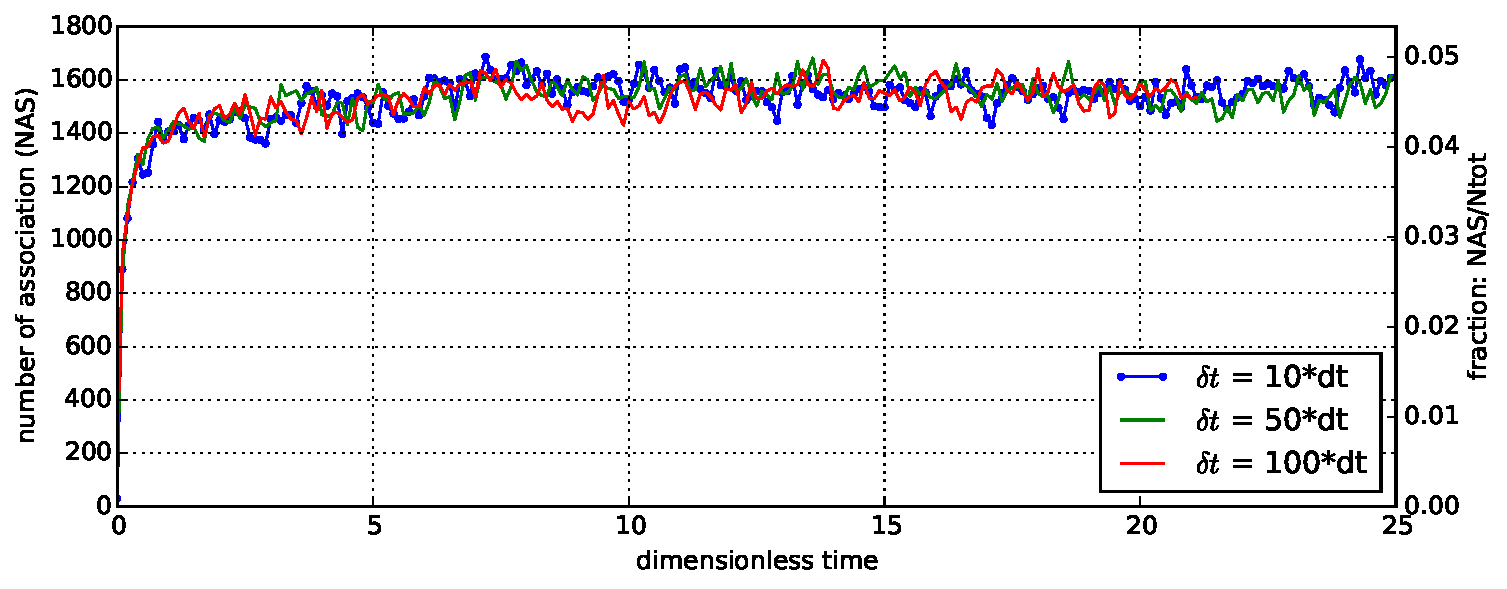
\includegraphics[width=\textwidth]{figures/NP1350_delta_t_test.pdf}
  \caption{Number of association with respect to topological dimensionless time. The different topological time step is applied and shows the given time step is not violate the topological evolution.}
  \label{fig:NP1350_NAS}
\end{figure}

\begin{figure}
  \centering
  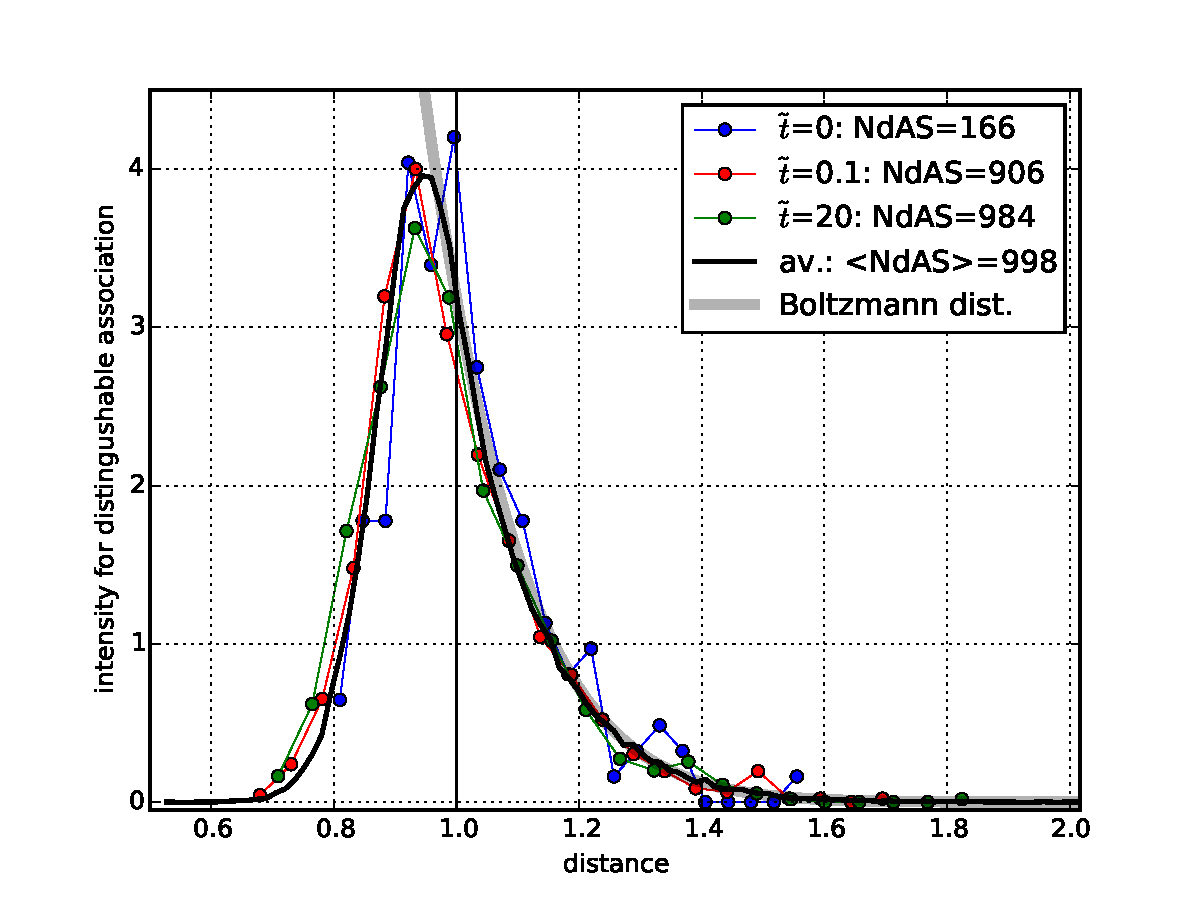
\includegraphics[width=\textwidth]{figures/check_Boltzmann_dist.pdf}
  \caption{Normalized histogram for association information with different time step (symbol), average over equilibrated time (black solid line), and theoretical expectation (gray line).}
  \label{fig:Boltzmann_dist}
\end{figure}

\begin{figure}
  \centering
  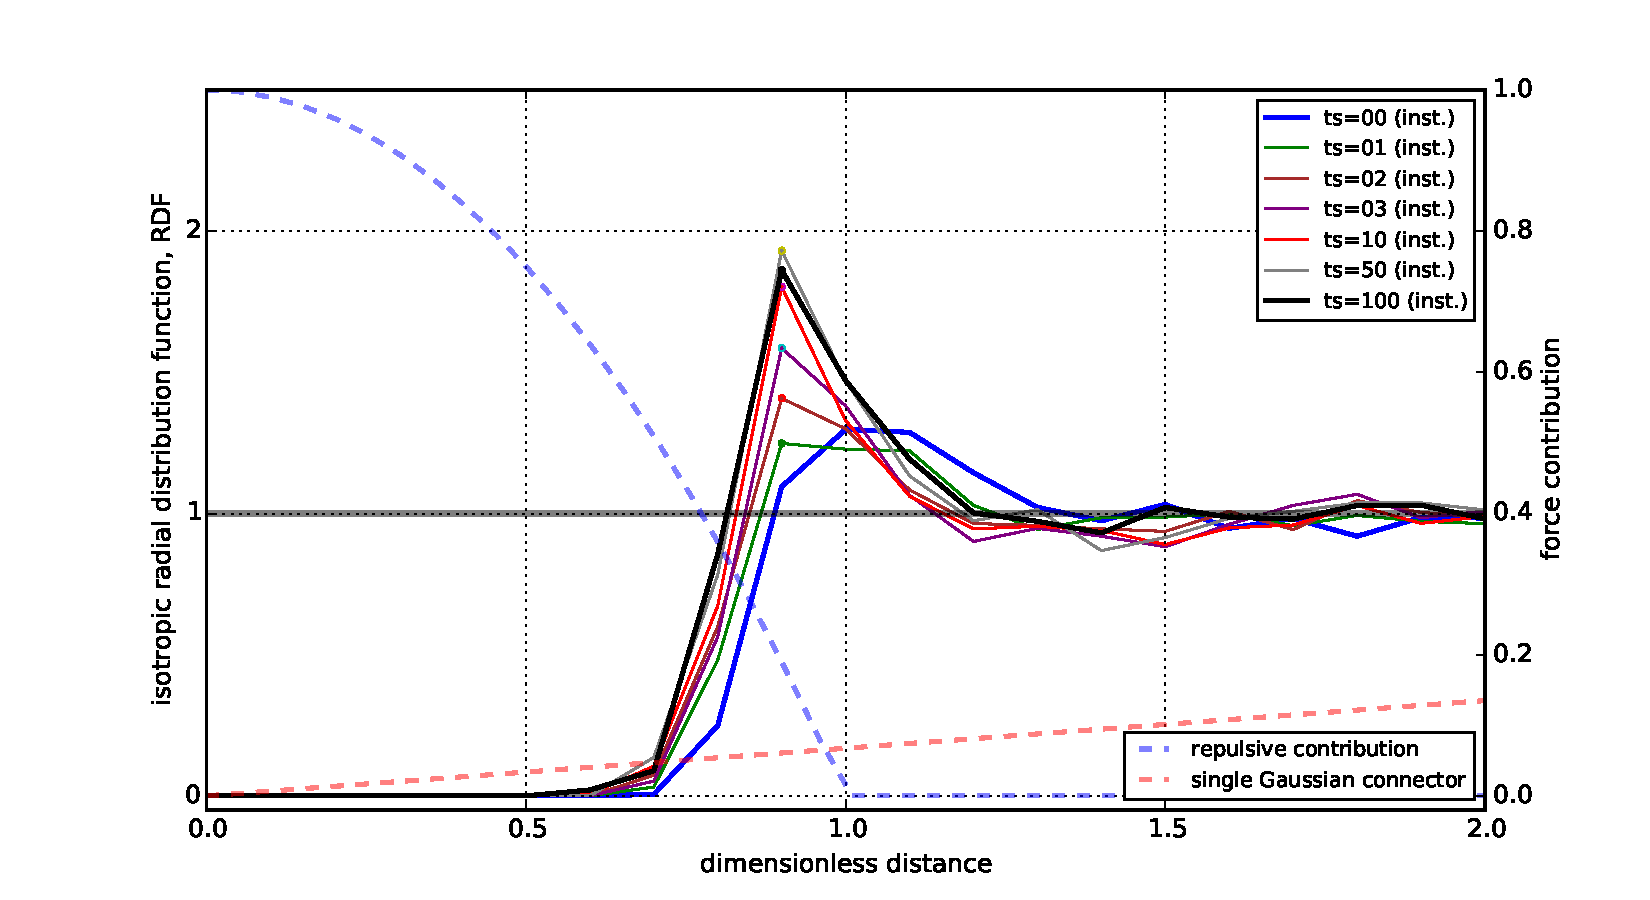
\includegraphics[width=\textwidth]{figures/RDF_NP1350_inst_EQ.pdf}
  \caption{Instantaneous radial distribution function with different time.}
  \label{fig:RDF_NP1350_INST}
\end{figure}

\begin{figure}
  \centering
  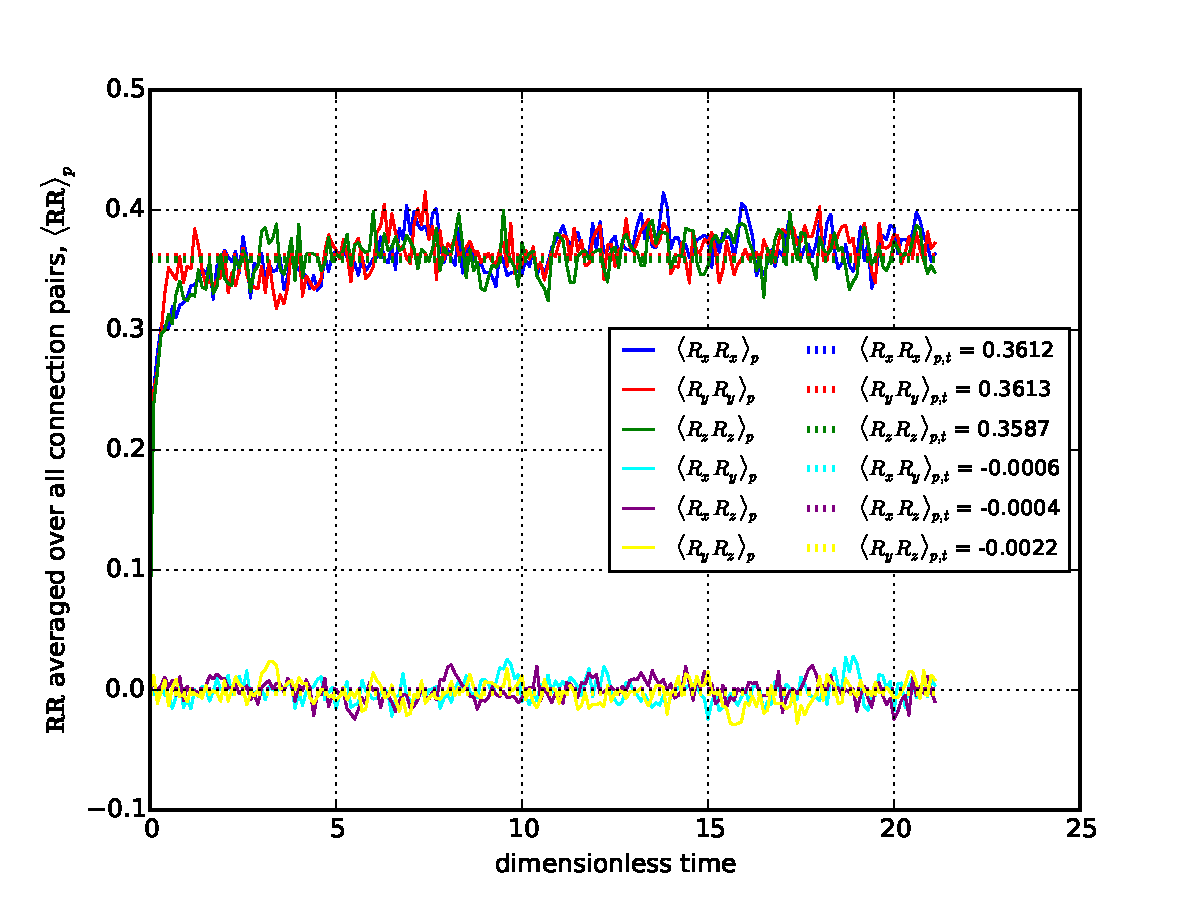
\includegraphics[width=\textwidth]{figures/NP1350_LD15P3_C100_averaged_RR.pdf}
  \caption{Isotropy test for 3D test.}
  \label{fig:isotropy}
\end{figure}


\section{Computational Economy}
\subsection{Frequency to Update Topology}
The simulation is composed of Brownian update and topological update, that spend a lot of time for topological update. Hence, if we increase the topological time step without violating association statistics, we can save big time. As we already have in the \eqref{eq:delta_t_criterion}, the topological time step can be from Brownian time step to reciprocal maximum value of detachment frequency. In addition, when the $\delta t$ decreases, the dissociation probability decreases since it linearly depends on the $\delta t$. Figure \ref{fig:topological_time_step_effect} shows how the criterion works and NAS suggest that there is no structural differences inside the criterion. To measure structural differences, the RDF have been checked for 0.01, 0.05, and 0.1 but without any differences. Recall the claim in local anisotropic effect for the topological time step argument, the figure significantly shows that the differences between normal (sparse) network structure and biased (dense) network structure. 

\begin{figure}
  \centering
  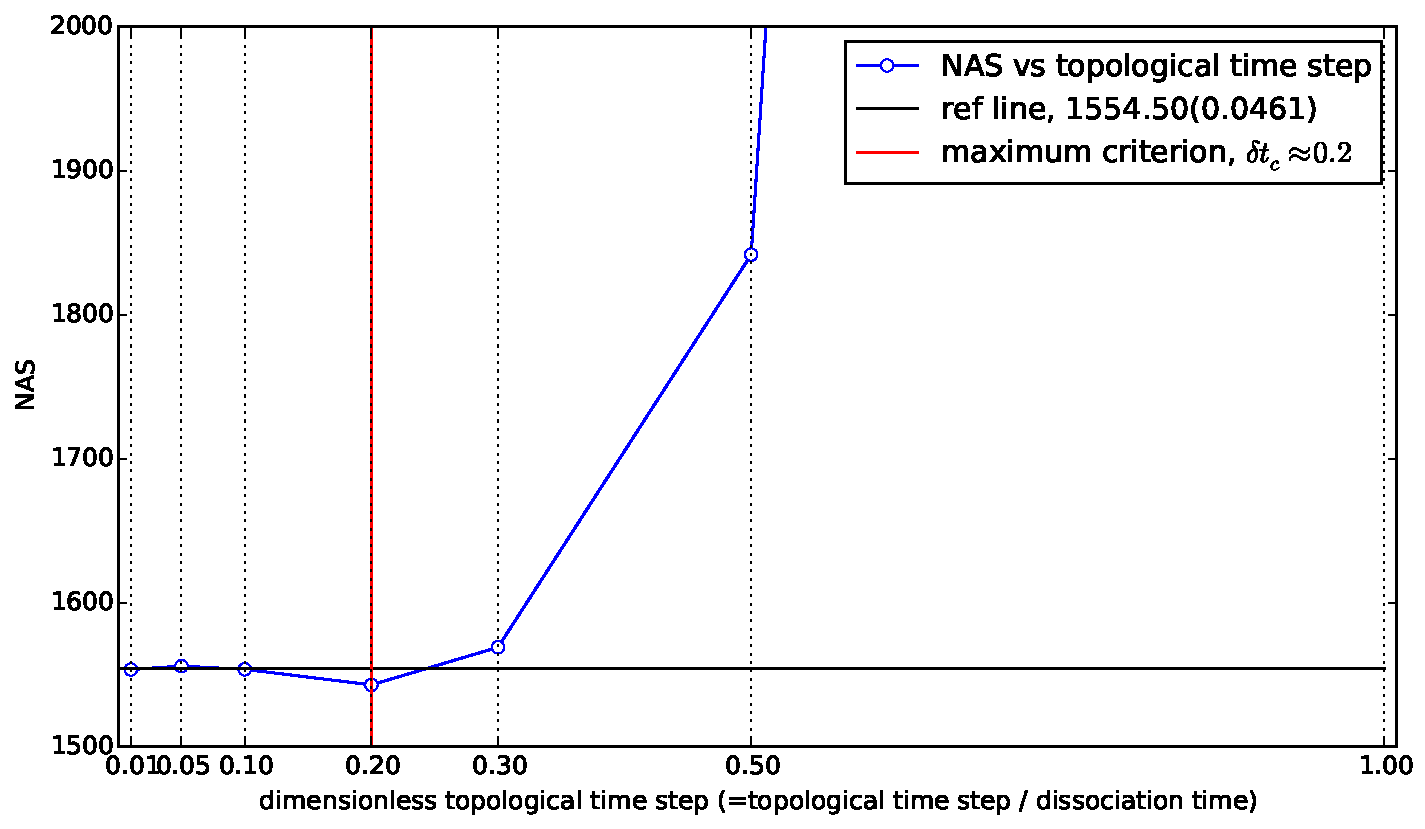
\includegraphics[width=\textwidth]{figures/compare_NAS_topological_time_step.pdf}\\
  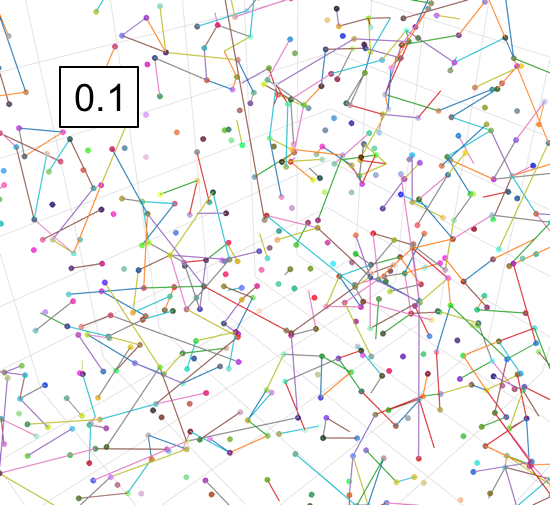
\includegraphics[width=0.45\textwidth]{figures/sparsely_aggregate.png}
  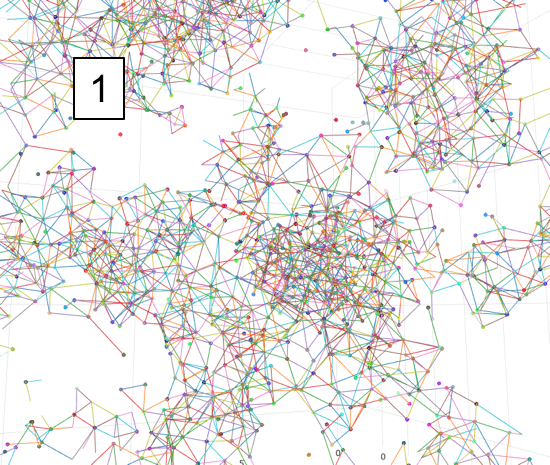
\includegraphics[width=0.45\textwidth]{figures/densely_aggregate.png}
  \caption{Effect of topological time step (up) to the associative system. The maximum distance for given association map is used to set the maximum criterion. The results of structure (down) for $\delta \tilde{t} = 0.1$ (left) and $\delta \tilde{t} = 1$ (right) are reported.}
  \label{fig:topological_time_step_effect}
\end{figure}

\subsection{Box Size Effect}
To use the minimum size that does not violate statistics is very useful to reduce computational time. For the default test set with micelle number density 0.4 have been tested with various box size. The figure \ref{fig:size_effect} suggest that various idea for the structural information is not changed due to decrease box size, while the computational time reduced dramatically since the same density, number of particles is reduced to 400 from 1350. Since most of computation for overhead without implementation of cell list becomes $N_p^2$, the asymptotically it is reduced by factor of 0.08. 

\begin{figure}
  \centering
  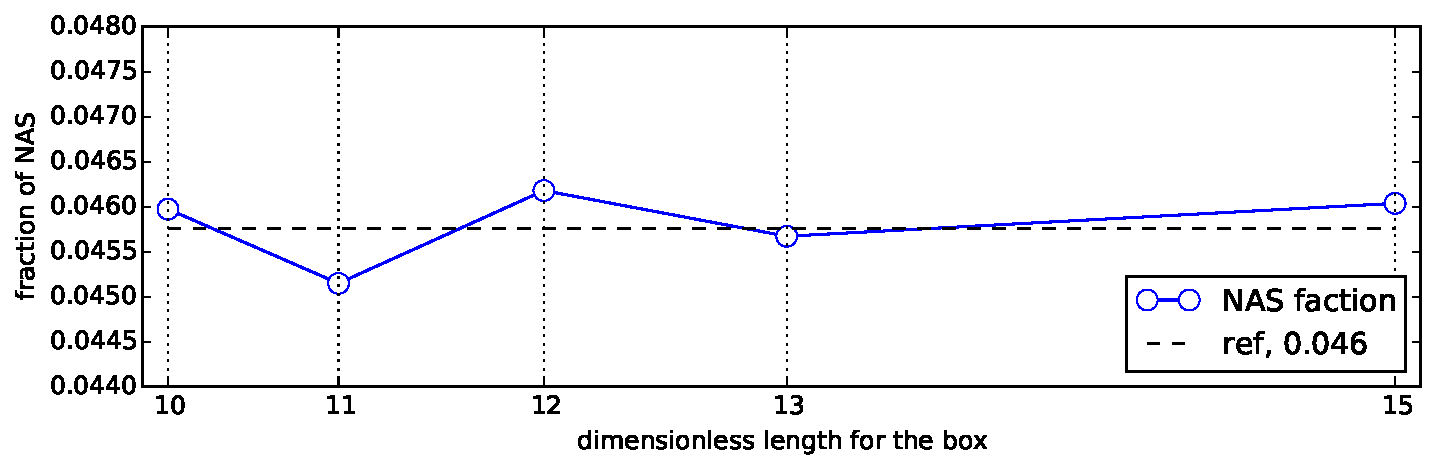
\includegraphics[width=\textwidth]{figures/plt_NAS_timestep.pdf}\\
  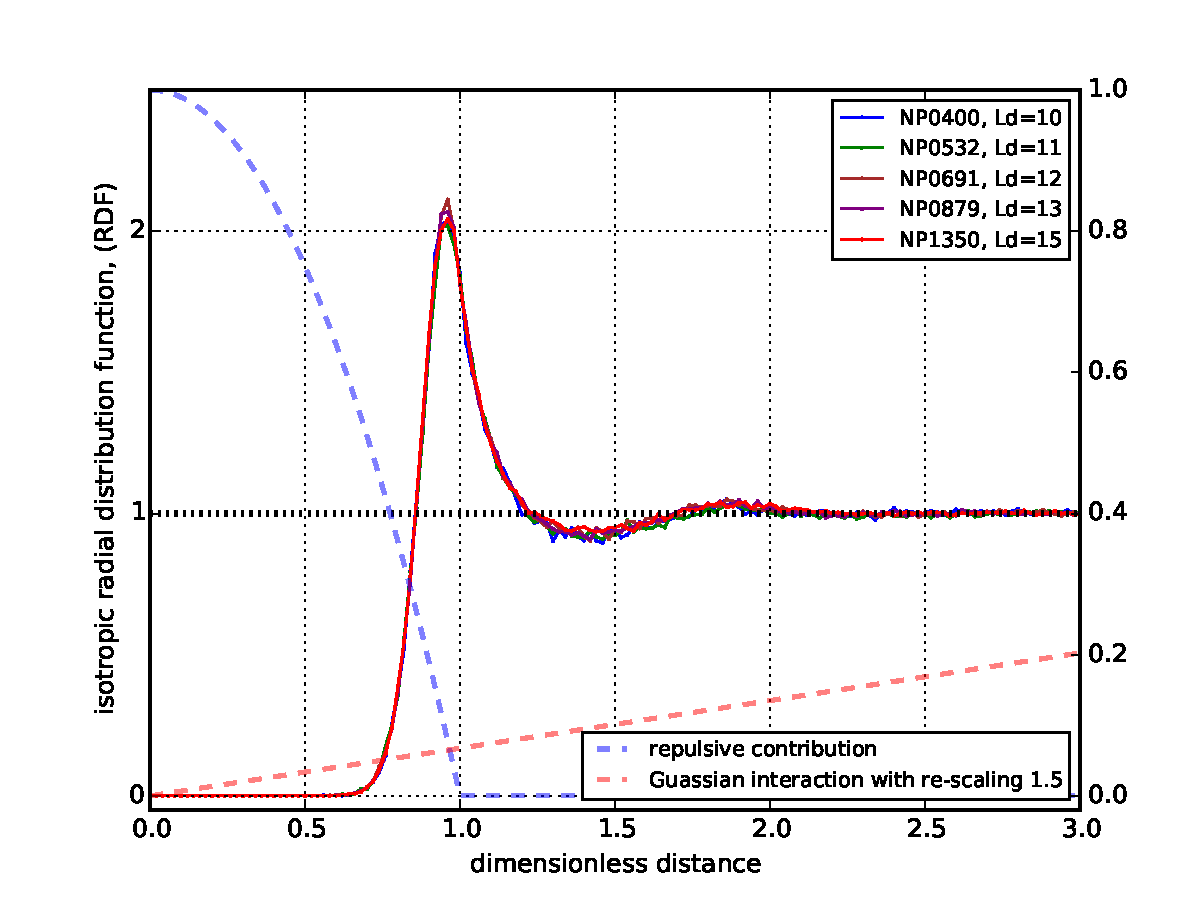
\includegraphics[width=0.7\textwidth]{figures/RDF_boxsize.pdf}\\
  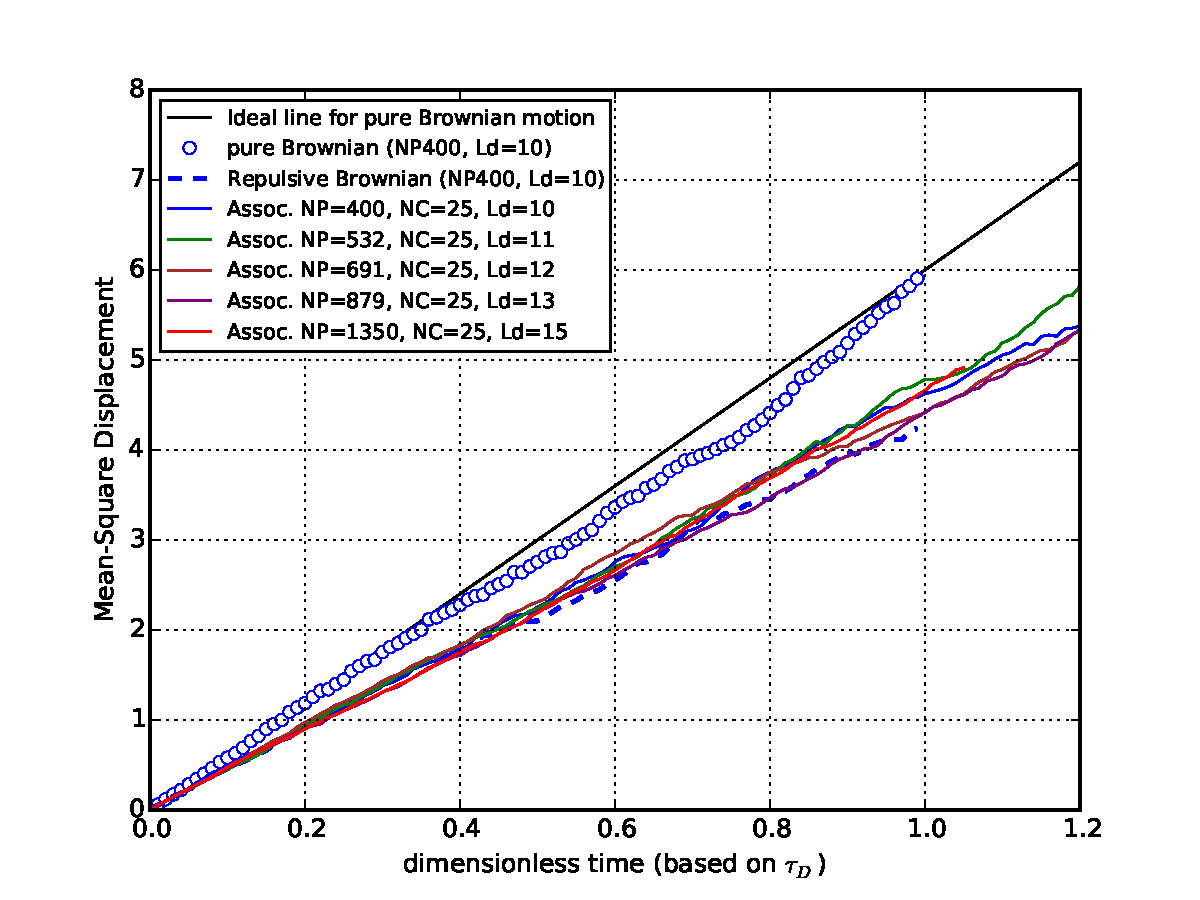
\includegraphics[width=0.6\textwidth]{figures/MSD_compare_LD.pdf}
  \caption{The fraction of number of association to the total chains on the box (up), the isotropic radial distribution function for different box size (middle), and mean-square displacement (MSD) with expected pure Brownian motion (down).}
  \label{fig:size_effect}
\end{figure}

\section{Finding The Relevant System}
\textcite{Suzuki:2012gfa} report the number density for active chain as $\nu \approx 3.7 \times 10^21 m^{-3}$ while the number density for the system as $\nu_0 \approx 1.8\times^{23}m^{-3}$. The ratio becomes 0.021, which means we have to find 0.021 of $N_{tot}$ is associated and the network shows the sparse network. This is not easy task since there are various parameter sets for our simulation such as the ratio between micelle size and end-to-end distance for single chain, $\alpha$ in the equation set, number density of micelles, number of chains per micelles, and number of allowance to fluctuate for micelles.

One easiest expectation might be increasing the number density of micelles, which will increase association. Figure \ref{fig:NAS_compare_NP_dependency} shows the dependency of fraction of number of association to the total number of chains in the box in terms of micelle density. The percolation identification is done the method depicted in \ref{sec:percolation_identification}, which in result, show figure \ref{fig:percolation_NP_dependency}.

\begin{figure}
  \centering
  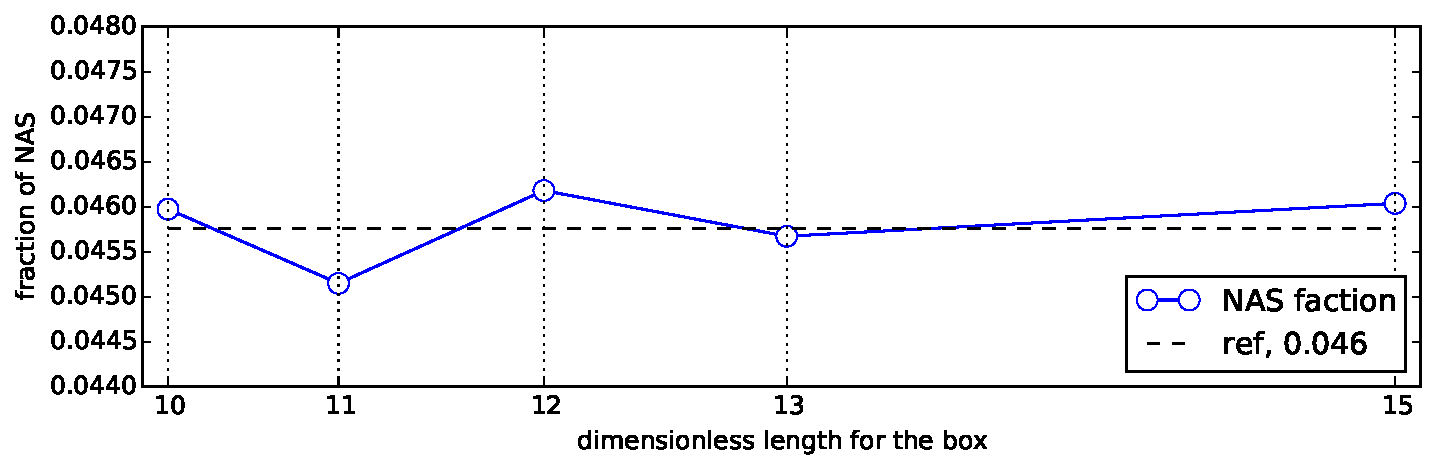
\includegraphics[width=\textwidth]{figures/plt_NAS_timestep.pdf}\\
  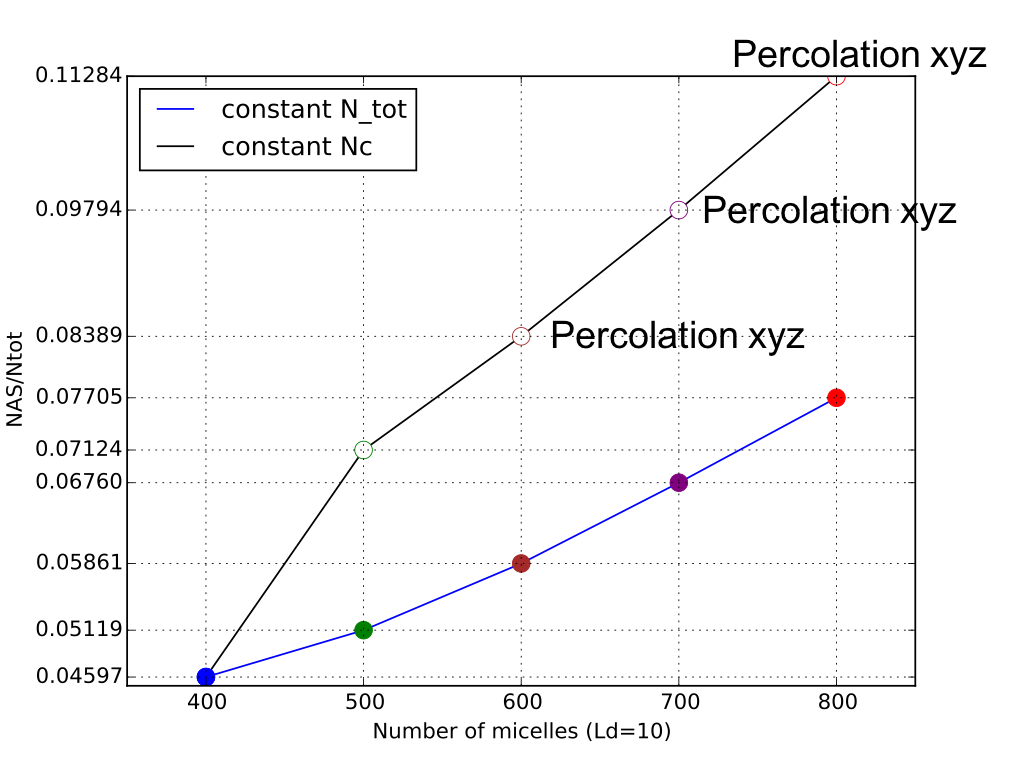
\includegraphics[width=0.7\textwidth]{figures/NAS_NP_dependence_percolation.png}
  \caption{Fraction of $N_{as}$ to the $N_{tot}$ (up). The solid line represent the same total number of chains in the box while the dashed line represent the same number of chains per micelles. The fraction vs. number of micelles (down) and percolation idenficiation.}
  \label{fig:NAS_compare_NP_dependency}
\end{figure}

\begin{figure}
  \centering
  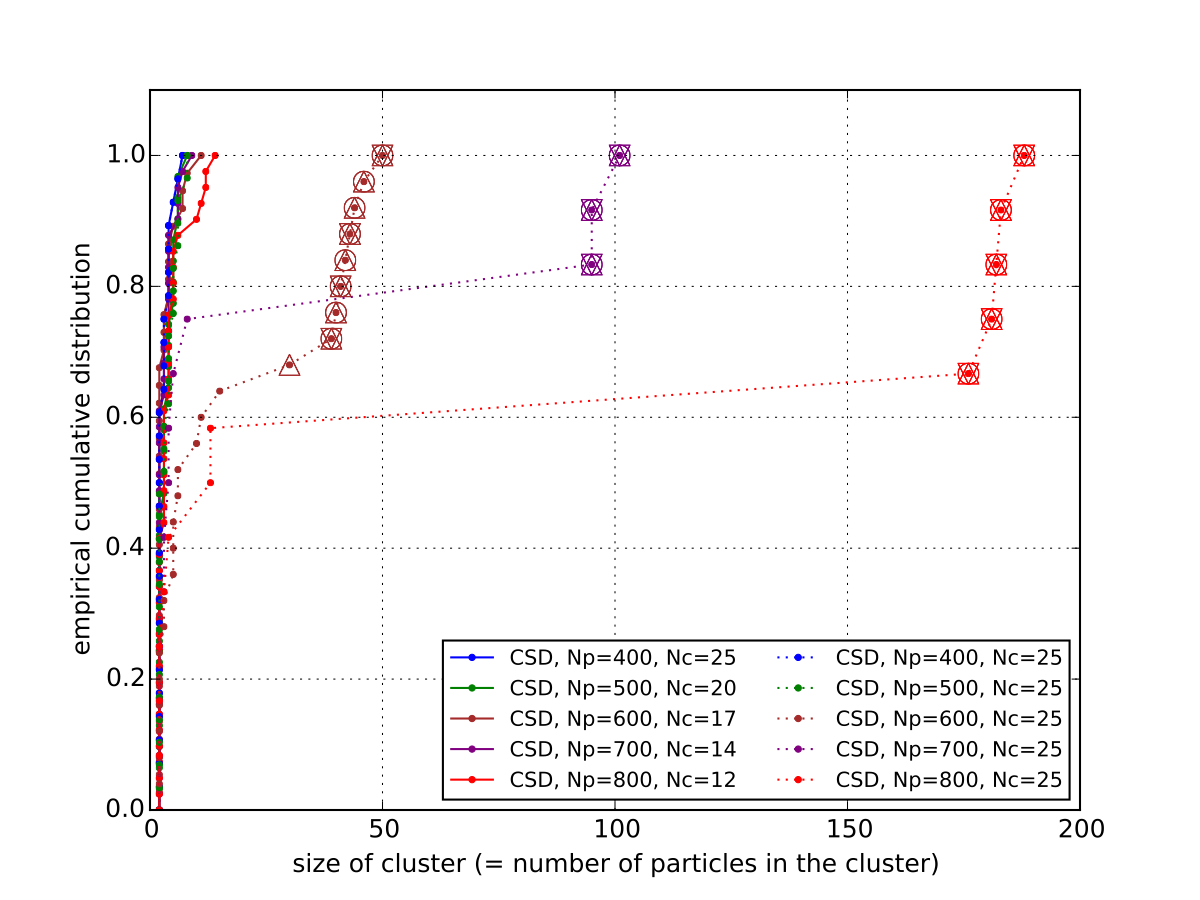
\includegraphics[width=\textwidth]{figures/percolation_NP_dependency.png}
  \caption{Cluster size distribution and test for the cluster's percolation properties. The DFS travel for vertex (including identification of edge) is used as depicted in \ref{sec:percolation_identification}. The dot denote existence of cluster, circle, upper triangle, lower triangle denote the given cluster percolate through X, Y, and Z axis, respectively.}
  \label{fig:percolation_NP_dependency}
\end{figure}



%% \subsection{Equilibrium Properties}
%% \subsection{Percolation Identification}
\section{Conclusions}
\begin{itemize}
\item The mechanism for shear thickening for HEUR solution is still in controversy
\item The different scaling law for dominant relaxation time and plateau modulus are reported \textcite{Uneyama:2012ge}
\item Developed stochastic simulation is studies in equilibrium structure and tested various aspect
\item Cluster size distribution and percolation identification are of importance to identify the network structure and bridge with the transient network model
\end{itemize}

\section{Future Works}
\begin{itemize}
\item More study about static condition of the network such as percolation identification, cluster size distribution, and number density of micelles and chains
\item Studies about model parameters are necessary such as repulsive contribution that depends on the number of chains per micelles
\item For computational economy, cell list will be implemented and the topological parallelization will be done through cell list
\item The Lee-Edwards boundary condition will be used for steady-shear flow, and the rheological quantities will be measured
\end{itemize}

  


\begin{appendices}


  \chapter{Software architecture}\label{appen_software_architecture}
  \section{GNU's scientific library as Front-End for Mathematical Calculations}
  The core for mathematical calculation is based on GSL with MKL interface supported by Intel composer. On this Brownian simulation, one of the most important feature is generating random noise. This is achieved using GSL's \href{https://www.gnu.org/software/gsl/manual/html_node/Random-Number-Generation.html}{Random Number Generation} packages that support efficient and sufficient white noise for our purpose. In addition, mathematical multiplication and various kinds of processing will be used based on matrix structure of GSL and also its linear algebra packages at the moment.

  If we need to achieve better performance, the matrix algebra will be replaced by cBLAS that is C-ported BLAS package, and linear algebra package will be replaced by LAPACK.

  \section{Math Kernel Library (MKL) as interface between Front- and Back-End}
  The MKL in Intel composer has functionality with its inter-facial function with various packages such as GSL, cBLAS, and LAPACK. Combining with the Intel compiler, the performance is reaching the one of the best in the numerical packages. The benefits of MKL is simple: support various package as their own style. 

  \section{Personally developed MATRIX class as Back-End}
  Not only the opensource packages, the personally developed MATRIX class is used because the core interface for GSL is not so convenience for scientific purpose. In addition, GSL is designed for C rather than C++, that means it is lack of advanced functionality such as operator overloading. Therefore, the core of GSL has high compatibility with various environment but low user-friendly. 

  The basic idea for developing MATRIX class is to overcome the shortage of connecting between mathematical formalism and code expressions. For instance, for given matrix $\mathbf{A}$, $\mathbf{B}$, and $\mathbf{C}$, when we calculate $\mathbf{A}\cdot\mathbf{B} + \mathbf{C}$ to input $\mathbf{C}$, using cBLAS, we need to use following sourcecode.
  \begin{lstlisting}[language=C++,frame=single,numbers=none]
    gsl_blas_dgemm(CblasNoTrans, CblasNoTrans, 1.0, &A.matrix, &B.matrix, 1.0, &C.matrix);
  \end{lstlisting}
  When we are using operator overloading with specialized object, than we can simply compute
  \begin{lstlisting}[language=C++,frame=single,numbers=none]
    C = A*B + C;
  \end{lstlisting}
  which is very simple and intuitive to use. Hence, I have developed several way to this expressions using operator overloading. Up to now, there is still performance issue since the equality operator (=) is internally generating new MATRIX object and returning it, that make overheads compared with the function to use call-by-reference style asGSL or cBLAS. To reduce this overhead is high rated for further refinement of sourcecode which will not be solved soon. For this reason, following operator overload is defined (only headerfile is included):
  \begin{lstlisting}[language=C++,frame=single]
    double& MATRIX::operator()(MKL_LONG i, MKL_LONG j);                 
    double& MATRIX::operator()(MKL_LONG i);
    MATRIX& MATRIX::operator=(const MATRIX &Mat);
    MATRIX& MATRIX::operator+=(const MATRIX &Mat);

    // MATRIX Addition : C = A+B
    MATRIX operator+(const MATRIX &A, const MATRIX &B); 
    MATRIX operator-(const MATRIX &A, const MATRIX &B); 
    // Scalar Multiplification : C = a*A
    MATRIX operator*(const double a, const MATRIX &A);  
    // MATRIX Multiplification : C = A*B
    MATRIX operator*(const MATRIX &A, const MATRIX &B); 

    // Unary operator
    MATRIX operator-(const MATRIX &A);                       
  \end{lstlisting}

  However, it should be notice that the operator overloading has potentially overhead for computing. At the moment for the Brownian particles, it is not that severe. 

  \section{Parsing Test Conditions}
  For general purpose program, parsing test condition cannot be avoidable. Here, The COND class is newly defined using C++ string class, that contains basic information of given condition file. I have attached one example for the test condition file as follow.
  \begin{lstlisting}[frame=single]
    Method=NAPLE_ASSOCIATION
Step=NO_EQUILIBRATION
Integrator=Euler
N_THREADS_BD=6
N_THREADS_SS=1
N_dimension=2
box_dimension=40.0  
dt=0.001
Nt=1100
Np=640
N_skip=10
output_path=data
filename_base=test
transition_probability=UNIFORM
chain_selection=UNIFORM
repulsion_coefficient=100
effective_distance=1.0
cutoff_connection=3.0
N_chains_per_particle=25
tolerance_allowing_connections=3
tolerance_association=0.01
allowing_multiple_connections=TRUE
N_max_steps=1000000
connector=Modified_Gaussian
scale_factor_chain=0.5
ratio_RM_R0=11
l_cap=0.12
MC_LOG=FALSE
N_steps_block=100
MC_renewal=TRUE
CONTINUATION_TRAJ=TRUE
CONTINUATION_CONNECTION=FALSE
CONTINUATION_TRAJ_FN=EQ_NP640_cutted.traj
CONTINUATION_HASH_FN=FALSE
CONTINUATION_WEIGHT_FN=FALSE

  \end{lstlisting}

  The parsing code is given by
  \begin{lstlisting}[language=C++,frame=single]
COND::COND(char* fn)
  {
    GIVEN_FILE.open(fn);
    long cnt = 0;
    string line, cond, val;
    while(getline(GIVEN_FILE, line))
    cnt ++;
    GIVEN_FILE.clear(); // since the previous get-line reach the EOF, this is bad-status. So, it need clear to use file object.
    GIVEN_FILE.seekg(0);
    N_arg = cnt; 

    arg = (string**) new string* [N_arg];
    for(long i=0; i<N_arg; i++)
        arg[i] = (string*) new string [2];

    cnt = 0;
    while(getline(GIVEN_FILE, line))
      {
        stringstream iss(line);
        getline(iss, cond, '='); arg[cnt][0] = cond;
        getline(iss, val, '\n'); arg[cnt][1] = val;
        cnt ++;
      }
    GIVEN_FILE.close();
    ERR = "ERR";
  }

  string& COND::operator()(string option_type)
{
  for(long i=0; i<N_arg; i++)
      if(arg[i][0] == option_type)
          return arg[i][1];
  cout << "Bad condtion " << option_type << endl;
  return ERR;
}
  \end{lstlisting}

  Note that the operator overloading is useful to handling the conditions. For instance, if we need the value for ``condition{\_}1'', we simply use COND(``condition{\_}1'') that return the value as string class. If we need C-style string, just use c{\_}str() method. In any case, checking conditional phrase is easily doable by following way.
  \begin{lstlisting}[language=C++, frame=single]
    if (given_condition("Integrator") == "Euler")
    {
      N_basic = 2;
    }
  \end{lstlisting}
  
  \section{Periodic Boundary Condition}
  \subsection{Minimum Image Convention}
    At the moment, only the rectangular PBC is under the consideration. When we computing some potential or distance, we have to account all image of particles with different cells. Without loss of generality with spatial dimension, the minimum is determined by following codes.
    \begin{lstlisting}[language=C++, frame=single]
      double UTIL_ARR::get_minimum_image_k_from_x(double x, double k, double dimension)
      {
        double kd[3] = {k-dimension - x, k - x, k+dimension - x};
        double re= kd[get_index_minimum_abs(kd, 3)] + x;
        return re;
      }

      MKL_LONG GEOMETRY::get_minimum_distance_pos_vector(TRAJECTORY& TRAJ, MKL_LONG index_t, MKL_LONG given_index, MKL_LONG target_index, MATRIX& given_vec)
      {
        for(MKL_LONG k=0; k<TRAJ.dimension; k++)
        {
          given_vec(k) = UTIL_ARR::get_minimum_image_k_from_x(TRAJ(index_t, given_index, k), TRAJ(index_t, target_index, k), TRAJ.box_dimension[k]);
        }
        return 0;
      }
    \end{lstlisting}
  \subsection{Applying Periodic Boundary Condition for Trajectory}
    The application of PBC on the trajectory is easily doable using the absolute value of coordinate. The sourcode is using 0 as origin, and all the box dimension is set as positive value from the origin. Therefore, it is needed to transit to make center as origin, taking modulo operator, then transit to original coordinate. The approach is described on the following codes.
    \begin{lstlisting}[language=C++, frame=single]
      MKL_LONG GEOMETRY::minimum_image_convention(TRAJECTORY& TRAJ, MKL_LONG target_t)
      {
        for (MKL_LONG i=0; i<TRAJ.Np; i++)
        {
          for (MKL_LONG k=0; k<TRAJ.dimension; k++)
          {
            double diff = TRAJ(target_t, i, k) - 0.5*TRAJ.box_dimension[k];
            double sign = diff/fabs(diff);
            if (fabs(diff) > 0.5*TRAJ.box_dimension[k])
            {
              TRAJ(target_t, i, k) -= sign*TRAJ.box_dimension[k];
            }
          }
        }
        return 0;
      }
    \end{lstlisting}
  
  \chapter{Parallel Computing}
  Up to now, the only shared memory parallization is supported via OpenMP package. In order to support GRID computing with multiple nodes, OpenMPI should be involved my sourcecode that is on queuing for further purpose. 

  It is noteworthy that OpenMP on the C++ has some importance issue to make private variable. Since I am using class instant for our convenience that described in above, the private class instance for OpenMP always call ``default constructor''. Because default constructor of MATRIX library is not compatible for further computing, it must be used in firstprivate rather than private. The option ``firstprivate'' is taking copy-constructor rather than default constructor.

  \section{Random Stream}
  The random number generation of this code is through GSL support (as MKL backend), which is NOT thread-safe. If we using the same stream with different thread, the generated random number will violate the statistics. On this regards, the pre-allocated stream-line for random number is used, and the number of stream-line is the same with number of thread (number of process in this code). By using this technique, we can avoid the violate random streaming. Near future, random generation by MKL will be implemented that is thread-safety. Note that, even if the MKL supported generator is thread-safe, it is necessity to use block-like streaming.
  
  
  \section{Brownian Update}
  For detail, see part of Euler Integrator in lib{\_}evolution.cpp file.
  \begin{lstlisting}[language=C++,frame=single]
    #pragma omp parallel for default(none) shared(TRAJ, POTs, CONNECT, index_t_now, index_t_next, R_minimum_vec_boost, R_minimum_distance_boost, vec_boost_Nd_parallel, force_spring, force_repulsion, force_random, r_boost_arr, N_THREADS_BD, given_condition) num_threads(N_THREADS_BD) if(N_THREADS_BD > 1)
      for (MKL_LONG i=0; i<TRAJ.Np; i++)
        {
          MKL_LONG it = omp_get_thread_num(); // get thread number for shared array objects
          
          force_spring[i].set_value(0);
          force_repulsion[i].set_value(0);
          force_random[i].set_value(0);

          if(given_condition("Step")!="EQUILIBRATION")
            INTEGRATOR::EULER_ASSOCIATION::cal_connector_force_boost(TRAJ, POTs, CONNECT, force_spring[i], index_t_now, i, R_minimum_vec_boost, R_minimum_distance_boost);
          INTEGRATOR::EULER::cal_repulsion_force_boost(TRAJ, POTs, force_repulsion[i], index_t_now, i, R_minimum_vec_boost, R_minimum_distance_boost);
          INTEGRATOR::EULER::cal_random_force_boost(TRAJ, POTs, force_random[i], index_t_now, r_boost_arr[it]);
          for (MKL_LONG k=0; k<TRAJ.dimension; k++)
            {
              TRAJ(index_t_next, i, k) = TRAJ(index_t_now, i, k) + TRAJ.dt*((1./POTs.force_variables[0])*force_spring[i](k) + force_repulsion[i](k)) + sqrt(TRAJ.dt)*force_random[i](k);
            }
        }
  \end{lstlisting}

  Because of overhead for copy constructor in the MATRIX class, all the internal variables are avoid the overloaded operator. The reference pass through pre-allocated objects are very fast in C++, but to reduce readability of the code. The way to implement copy constructor inside of operator overload without overhead will be considered in future.

  \subsection{Parallelization Topological Update}
  \subsubsection{LOCKING Bead}
  The parallelzation for Brownian update is very simple as depicted in above. In the case for topological update, however, it is quite tricky because of parallelization potentially violate the statistics of randing picking - dissociation - association chains. On this regards, LOCKING mechanism is introduced that means whenever the beads are in-visited state, the bead is locked until the processing on the bead is done. The main parts of locking is described in the below code. The check is through the OpenMP critical directive, which means the only one process allowed to enter following bracket. However, this scheme make strong overhead to reduce the efficiency of parallelization. For instance, the computation time for topological update is 2.5 when we use 6 processors. 

  \begin{lstlisting}[language=C++,frame=single]
#pragma omp critical(LOCKING)  // LOCKING is the name for this critical blocks
              {
                /*
                  On the omp critical region, the block will work only one thread.
                  If the other thread reaching this reason while there is one thread already working on this block, then the reached thread will wait until finishing the job of the other thread.
                  This benefits to identify the working beads index on this case, since the 
                */
                // CHECKING
                for(MKL_LONG I_BEADS = 0; I_BEADS < 3 && N_THREADS_SS > 1; I_BEADS++)
                  {
                    if(LOCKER(IDX_ARR[it].beads[I_BEADS]))
                      {
                        IDENTIFIER_ACTION = IDX_ARR[it].CANCEL;
                        IDENTIFIER_LOCKING = TRUE;
                        break;
                      }
                  }
                // this is LOCKING procedure
                if(!IDENTIFIER_LOCKING)
                  {
                    cnt++;  // preventing LOCKING affect to the IDENTIFICATION of stochastic balance
                    for(MKL_LONG I_BEADS = 0; I_BEADS < 3 && N_THREADS_SS > 1; I_BEADS++)
                      {
                        LOCKER(IDX_ARR[it].beads[I_BEADS]) = TRUE;
                      }
                  }
                else
                  {
                    cnt_lock ++;
                  }
              }

  \end{lstlisting}
  \subsubsection{TODO Cell Lists Parallelization}
  Since implementation of the cut-off scheme through cell lists is on queue, it is much efficiency compared with the suggested LOCKING procedure. The cell list composed of different block of cells inside the box and the cell dimension is higher than cut-off radius. On this scheme, to pick beads inside the different cell does not violate the statistics. The implementation will be done in future.
\chapter{Data Structure for Connectivity Information}
\section{Multi-dimensional Array}
\label{sec:orgheadline2}
For compatibility and convenience, the multi-dimensional arrays are expressed by one-dimensional array by index mapping function. To be specific, the given N by M 2-dimensional array may have the form of table \ref{tab:orgtable1}, which is possibly mapped to table \ref{tab:orgtable2}. The advantage for this expression can be thought as two parts: coding interface can be united and we can use several compression techniques such as lower occupation for symmetric matrix. There are various numerical packages have been used this way: BLAS, LAPACK, GSL, and so on.


\begin{table}[htb]
\caption{\label{tab:orgtable1}
Example for typical 2-dimensional array}
\centering
\begin{tabular}{cccccc}
index & 0 & 1 & 2 & \(\cdots\) & M\\
\hline
0 & val(0,0) & val(0,1) & val(0,2) &  & val(0, M)\\
1 & val(1,0) & val(1,1) & val(1,2) &  & val(1, M)\\
 &  & \(\vdots\) &  & \(\ddots\) & \\
N & val(N,0) & val(N,1) & val(N,2) &  & val(N,M)\\
\end{tabular}
\end{table}

\begin{table}[htb]
\caption{\label{tab:orgtable2}
Example for mapping to 1-dimensional array from 2-dimensional array.}
\centering
\begin{tabular}{cccccccc}
index & 0 & 1 & \(\cdots\) & M & M+1 & \(\cdots\) & NM\\
\hline
coord. & (0,0) & (0,1) & \(\cdots\) & (0,M) & (1,0) & \(\cdots\) & (N,M)\\
\hline
val. & val(0,0) & val(0,1) & \(\cdots\) & val(0,M) & val(1,M) & \(\cdots\) & val(N,M)\\
\end{tabular}
\end{table}



\section{Adjacency Matrix and List}
\label{sec:orgheadline3}
Consider the given association information, we can easily express the information using adjacency matrix:
\begin{equation}
\mathbf{C}_m = \left[\mathscr{C}_{ij}\right],
\end{equation}
where \(\mathscr{C}_{ij}\) is number of associations for the pair of i- and j-th particles.
The expression is quite simple and it contains all the existing information. However, the adjacency matrix is expensive both of time and space complex because adjacency matrix explicitly denote zeros inside the array, which needed more time for zero identification during processing. Hence, the adjacency list have been used :
\begin{equation}
\mathbf{C}_l = \left[\mathscr{I}_{i}(j)\right],
\end{equation}
where i denote the index for subject particle, j denote index for columns, and \(\mathscr{I}_{i}(j)\) is the index that is j-th connection to the i-th particle. 
For instance, consider the given network has the form of figure \ref{orgkeyword1}, then the adjacency matrix becomes table \ref{tab:orgtable3} and the adjacency list is expressed in table \ref{tab:orgtable4}. Note that the weight for the bridge should be stored in separated array for adjacency list.

\begin{figure}
\centering
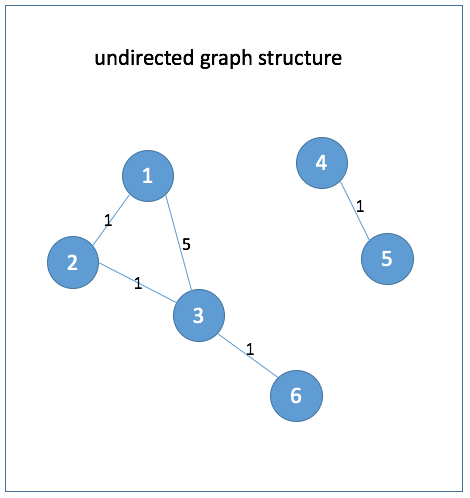
\includegraphics[width=.5\linewidth]{../data_structure/ex_graph_association.png}
\caption{Example for association maps. It can be regarded as undirected graph since there is no directional information for the association (edge as CS notation) between particles (vortex as CS notation).}
\label{orgkeyword1}
\end{figure}


\begin{table}[htb]
\caption{\label{tab:orgtable3}
Example of adjacency matrix for figure \ref{orgkeyword1}.}
\centering
\begin{tabular}{rrrrrrr}
 & 1 & 2 & 3 & 4 & 5 & 6\\
\hline
1 & \(N_1\) & 1 & 5 & 0 & 0 & 0\\
\hline
2 & 1 & \(N_2\) & 1 & 0 & 0 & 0\\
\hline
3 & 5 & 1 & \(N_3\) & 0 & 0 & 1\\
\hline
4 & 0 & 0 & 0 & \(N_4\) & 1 & 0\\
\hline
5 & 0 & 0 & 0 & 1 & \(N_5\) & 0\\
\hline
6 & 0 & 0 & 1 & 0 & 0 & \(N_6\)\\
\end{tabular}
\end{table}

\begin{table}[htb]
\caption{\label{tab:orgtable4}
Example of adjacency list for figure \ref{orgkeyword1}.}
\centering
\begin{tabular}{rrrr}
bead & 0 & 1 & 2\\
\hline
1 & 2 & 3 & 0\\
2 & 1 & 3 & 0\\
3 & 1 & 2 & 6\\
4 & 5 & 0 & 0\\
5 & 4 & 0 & 0\\
6 & 3 & 0 & 0\\
\end{tabular}
\end{table}

\section{Identification for Percolation}
\label{sec:percolation_identification}
The percolation for one spatial dimension can be solved by travel algorithm for undirected graph structure in the word of computer science. The idea is to travel through all the bridge that connected the subjected particle, then identify the travel goes beyond box or not. 


\subsection{Travel Beyond Box Boundary}
\label{sec:orgheadline6}
\subsubsection{Minimum Image Convention}
\label{sec:orgheadline4}
Before going further, it is better to mention that the minimum distance between particles in periodic boundary condition (PBC) is using component-wise minimization:
\begin{equation}
\label{eq:orglatexenvironment1}
r^{(m)}_k(\mathbf{r}_i, \mathbf{r}_j) = \min\left\{x_k(\mathbf{r}_j) - \left(L_D\mathscr{S} + x_k(\mathbf{r}_i)\right)\right\},
\end{equation}
where \(k\) denote the k-th spatial dimension and \(L_D\) is box dimension and the shift set is given by \(\mathscr{S} = \{-1, 0, +1\}\),
which implies the relative vector of minimum distance from \(\mathbf{r}_j\) to \(\mathbf{r}_i\) is
\begin{equation}
Crd_{\varepsilon}\left(\mathbf{r}^{(m)}(\mathbf{r}_i, \mathbf{r}_j)\right) = [r_1(\mathbf{r}_i, \mathbf{r}_j), \cdots, r_{N_D}(\mathbf{r}_i, \mathbf{r}_j)]^T,
\end{equation}
where \(\varepsilon\) is given basis set. Minimum distance is simply given by Euclidean norm of this relative vector of minimum distance.

\begin{figure}
\centering
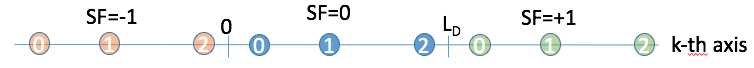
\includegraphics[width=.9\linewidth]{../data_structure/comp_minimum_distance.png}
\caption{Component-wise minimum distance relative vector}
\label{orgkeyword2}
\end{figure}

Let assume that we have 3 particles and the subject particle is zero, which depicted figure \ref{orgkeyword2}. If we started with 0th particle and try to find its the minimum distance with 2nd particle. For this processing, we have to count its the images of 2nd particle which can be in left or right side. The meaning of real left and right is not important because the axis independence. This is exactly the same meaning with equation \ref{eq:orglatexenvironment1} since
\begin{equation}
d^{(m)}_{ij} = \left|\mathbf{r}^{(m)}(\mathbf{r}_i, \mathbf{r}_j)\right|_2 = \sqrt{\sum_{k=1}^{N_d} (r^{(m)}_k(\mathbf{r}_i, \mathbf{r}_j))^2}
\end{equation}
becomes minimum when each \(r^{(m)}_k\) is minimum. Notice that this happens because of orthonormal basis. \emph{For general basis set, it is of importance that we have to measure component based on reciprocal base vector, which will be involved when the system is experienced shear.} 

\subsubsection{Identifier for Boundary Travels and Percolation}
\label{sec:orgheadline5}
For each travels, we can count shift factor for individual axis. If all the shift factors are zeros, it means the travel will happen inside of box. If k-th dimension has left (-1) or right (+1) shift factor, then the given travel goes beyond left or right boundary of k-th axis, respectively. In one cluster, the percolation through k-th axis happens when it travel both of left and right boundary.

\subsection{Travel Algorithm}
\label{sec:orgheadline11}
\subsubsection{Travel for Vertex: Measuring Cluster Size Distribution}
\label{sec:orgheadline7}
Let say cluster as the group of particles that is connected. The size of cluster is defined by number of particles on the subjected cluster, then we can measure cluster size distribution of given system. 

The given associated network has the same structure with the undirected graph that is composed of vertexes (particles in this case) and edges (association in this case). Undirected means that bridge chain is symmetric under the index of pair of particles, \(\mathbf{r}_{ij} = \mathbf{r}_{ji}\). Extracting information of association topology is done through traveling the network and the data is given by adjacency list. In general, depth-first search (DFS) and breadth-first search (BFS) are good for this aspect with different spanning tree. The details of the data structure and algorithm are described on Appendix. 



\subsubsection{Travels for Edges: Identify Travels Beyond PBC Box}
\label{sec:orgheadline8}
Travel for vertex means we visit all the particles that connected with the given root particle, but it does not guarantee that visiting all the edges (bridges). The percolation identification depends on the bridges, not about particles itself, which means we need to modify travel algorithm. There are various way to travel edges rather than vertex, but we need only information of edge not about real travels. Hence, the algorithm is slightly modified to record the identifier for shift factor for all the possible travel path - but do not act the travel when the target particle is already in-visited status. 

\subsubsection{Travels inside PBC Box}
\label{sec:orgheadline9}
As already mentioned in above, the travel is only allowed inside box and whenever travel is experienced beyond box, travel is canceled and it will be recorded for percolation identification. To be specific, consider the networks in figure \ref{fig:orgparagraph1} shows that different percolation scheme. However, the percolation through x axis in the (b) of figure \ref{fig:orgparagraph1} cannot be captured by given scheme since the percolation line through the boundary of subjected box. For relatively large 3-dimensional box, the situation is not so common, which is the reason to use introduced identification procedure. 

\begin{figure}
\centering
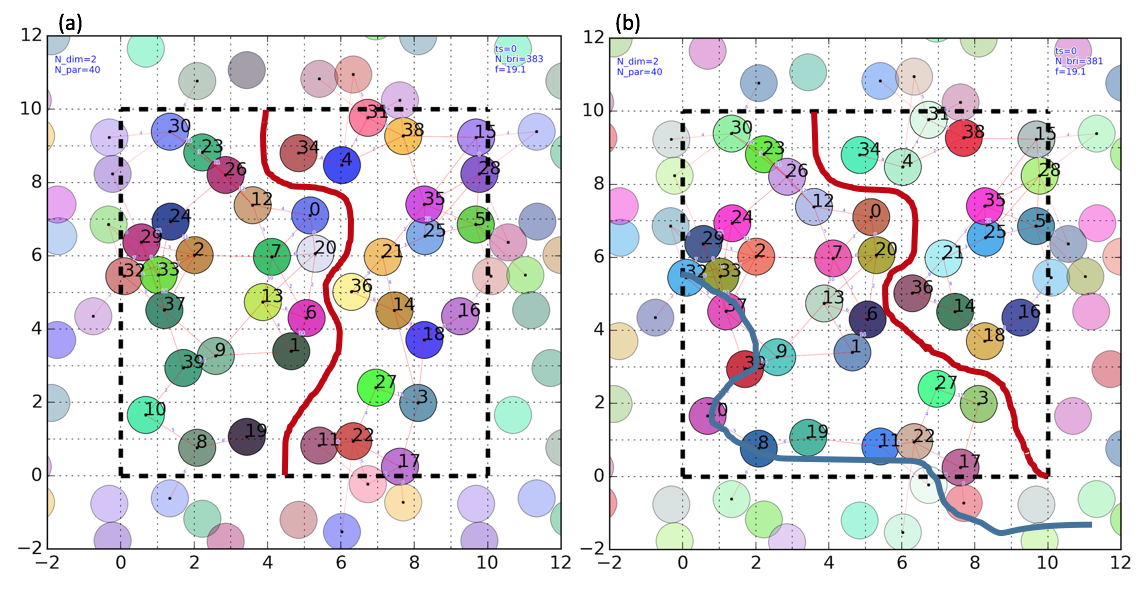
\includegraphics[width=.9\linewidth]{../data_structure/ex_percolation_identification.png}
\caption{
  Two dinsintuishable 2-dimensional cluster system. Left figure (a) represent percolation happens along y axis while no percolation along x axis. Right figure (b) represent the percolation happens both of x and y axis, but x percolation line beyond the subjected box. The thick red line represent isolation while the thick blue line represent percolation line along x axis.}
\label{fig:orgparagraph1}
\end{figure}

It also works well for 3-dimensional case. The given association information depicted in \ref{fig:orgparagraph2}. By eyes, it is not easy to judge there exist percolation cluster or not. From this algorithm, it reveals that the root index 0 is composed of 191 pairs of association that percolated along all the axis: x, y, and z. If we measure cluster size distribution and identify the given cluster is percolated with specified axis or not, the figure \ref{fig:orgparagraph3} is good point to observe. There are 60 distinguishable clusters and 2122 total number of particles in 60 clusters. Since the number of distinguishable association is 6022, 3900 particles are isolated or attached to wall. For detail distribution, the travel should be allowed for directed image (which will be implemented later) then the distribution will be more accurate.

\begin{figure}
\centering
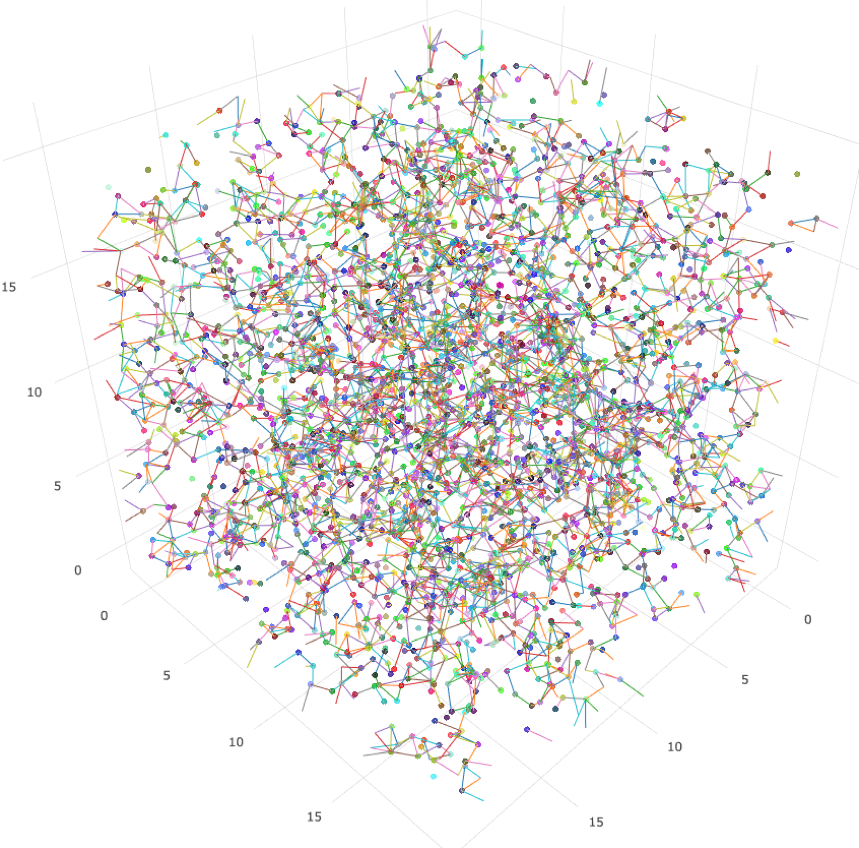
\includegraphics[width=.9\linewidth]{../data_structure/ex_3d_NP3200_SF20_percolation.png}
\caption{
  Equilibrium topology with the given condition: 3200Np, \(20^3\) dimensionless volume, 25 chains per each particle. Re-scaling factor is used 2.0.}
\label{fig:orgparagraph2}
\end{figure}

\begin{figure}
\centering
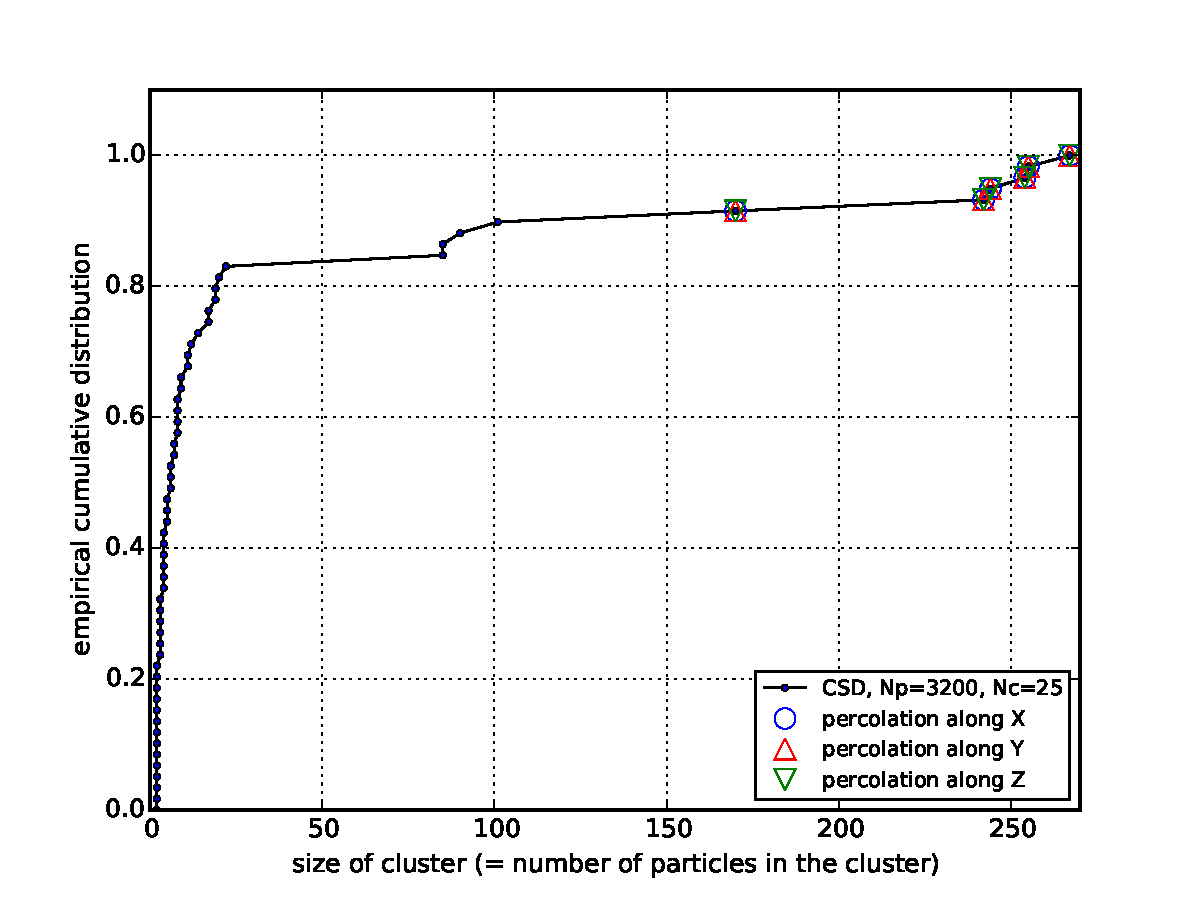
\includegraphics[width=.9\linewidth]{figures/test_percolation.pdf}
\caption{Empirical cumulative distribution for cluster size distribution. Percolation denoted by symbols for each axis, respectively.}
\label{fig:orgparagraph3}
\end{figure}



\subsubsection{{\bfseries\sffamily TODO} Allowing Travel Beyond Boundary of Box}
\label{sec:orgheadline10}
Notice that the following article is description for the idea. The alogirthm is not fully implemented into sourcecode, which will achieve later progress.

It might be more general way to allow travel beyond boundary of box. At this moment, there are several difficulties to allow such a travels. The most importance question is \emph{how to identify percolation}.

Allowing one more image of the subjected box is a key to identify percolation. During travels, we have to record all the parity of the travel identifier since it is a key of image. Sum of all travel identifier for a given axis, say image identifier, should not lower than -1 and higher than +1, which means only direct image of subjected box will be accounted. It is of importance to distinguish between particles in different box even if they have the same index number, which can be achieved using image identifier:
\begin{equation}
I^{k} = \sum_{i=1}^{N_{tb}} s^{k}_i,
\end{equation}
where \(N_{tb}\) is number of travel beyond boundary, k denote k-th spatial dimension and \(s^k_i \in \mathscr{S}\). It is quite simple that the image identifier, \(I^{k}\) can be any value of \(\mathscr{S}=\{-1, 0, +1\}\), which direct the current travel happens in the left, center, or right side of the box, respectively. Therefore, \emph{recorded shift factor is not the instance shift factor but sum of all instance shift factors.} Note that the travel to image particle is allowed even if its original particle in current PBC box is visited status. Once the travel is finished, all the particles in its direct image have been visited status and we have to make sure the all the edges are accounted for identification of travel. 

The identifier for this case is the same with travel identifier inside box: one cluster for k-th axis shows both of left and right imaginary shift factor, this is percolated. We do not need to travel further from direct image of current box. For simplification, the index vector is introduce:
\begin{equation}
\mathbf{I} = [i_1, i_2, i_3]^T,
\end{equation}
where \(i_1, i_2, i_3\) are the index for each axis. If the subjected particle is in current PBC box, the components are \(i_1 = i_2 = i_3 = i\) where i is the original index for the particle. If it is in directed image of PBC box, we can use shifted index:
\begin{equation}
i_k = i + S_k N_p,
\end{equation}
where \(S_k\) is the shift factor for the given axis and \(N_p\) is number of particles. For instance, if the system has 10 particles inside PBC box, then the \(i_k\) value becomes -10 to 20: -10 to -1 for the left image of k-th axis, 0 to 10 for the current box, and 11 for 20 for the right image of k-th axis. The mapping function from image of box to current box is easily given by \(i_k\) modulo \(N_p\): \(i_k\% N_p\). This benefit to record and tracking the stack memory of the iterative DFS algorithm.





\subsection{Python Code for Measuring Cluster Size and Percolation Identification}
\label{sec:orgheadline12}
There are various way to develop DFS algorithm for tree structure in general way. It is quite simple to use recursive form since DFS is using call stack. With given size of cluster, however, the recursive call is limited by system for safety reason, and have potential overhead because of calling functions typically taking time. On this regards, the code is developed by iterative manner with some set of if-phrase in order to identify edge travels. The code is described on code \ref{orgsrcblock1} written by python. The root index will be given by the argument index (default is zero). When we need to travel all the sub-graph of given graph (existing several clusters), we can iterate root index from zero to number of particles, then we can extract distinguishable clusters, which is the way to measure cluster size distribution.



%% \chapter{Appendix}
%% \label{sec:orgheadline16}
\subsection{Graph}
\label{sec:orgheadline14}
Mathematically, a graph is an ordered pair \(G = (V, E)\) where a set \(V\) of vertices and a set \(E\) of edges. 

For instance, we have vertices and edges for figure \ref{orgkeyword3} as 
\begin{align}
V &= \{0, 1, 2, 3, 4, 5\}\\
E &= \{(0, 1), (0, 3), (1, 2), (2, 4), (2, 5), (3, 4), (4, 5)\},
\end{align}
which in consequence \(V\) is set of all the index for particles and \(E\) is set of all pairs of index for bridges. It is of importance that the identification of percolation is not necessary to count weight on the bridge, i.e., number of connections for the same bridge, so we do not need count all the weight array on this graph analysis. In addition, the given graph is undirected since all the element for \(E\) is symmetric under the pair index: \((i, j) = (j, i)\). 

\begin{figure}
\centering
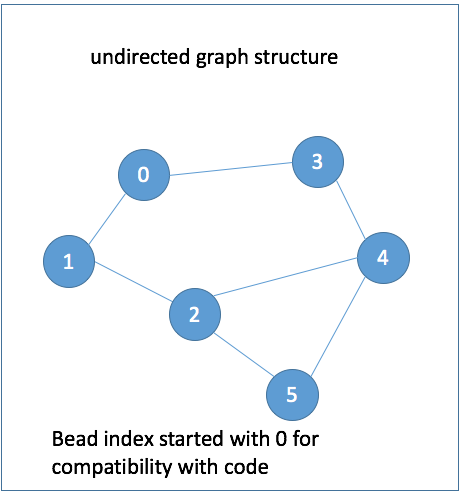
\includegraphics[width=.9\linewidth]{../data_structure/ex_graph_DFS.png}
\caption{Example for association maps. This example will be used DFS testing and the starting index  changed to 0 from 1 for compatibility with the code infrastructure. Therefore, index zero indicate the zero-th particle and -1 indicate there is no association.}
\label{orgkeyword3}
\end{figure}

\subsection{Tree and Spanning Tree}
\label{sec:orgheadline15}
Tree is linearized graph, which means graph without any circle of bridges. For given network structure is not tree because of association can happens to make loop. To understand tree structure, however, is of importance since the algorithms to travel graph is based on the tree. Basically, the graph cannot be merged to tree structure, but if we ignore loop bridges, we can span tree structure from given graph which is called \emph{spanning tree}. In consequence of linearization, the spanning tree is not unique that depends on the algorithms to travel. 

To be specific, for graph depicted in figure \ref{orgkeyword3}, if we apply DFS algorithm, the spanning tree has the form of figure \ref{orgkeyword4}. Here, the 0-th particle is selected as root, and the rank of child is represented by depth from root. If we use BFS algorithm, the spanning tree has different form like figure \ref{orgkeyword5}. The travel sequence for DFS becomes \(0\to 1\to 2\to 4\to 3\to 5\) while BFS becomes \(0\to 1\to 3\to 2\to 4\to 5\). In principle, the spanning tree is not necessary to generate but it is good way to understand the properties of given graph. Since DFS is used as default, this article only contains details about DFS. The adjacency list for the given graph is described in table \ref{tab:orgtable5}.

\begin{table}[htb]
\caption{\label{tab:orgtable5}
Adjacency list for the given graph, figure \ref{orgkeyword3}}
\centering
\begin{tabular}{rrrr}
 & 1 & 2 & 3\\
\hline
0 & 1 & 3 & -1\\
1 & 0 & 2 & -1\\
2 & 1 & 4 & 5\\
3 & 0 & 4 & -1\\
4 & 2 & 3 & 5\\
5 & 2 & 4 & -1\\
\hline
\end{tabular}
\end{table}

\begin{figure}
\centering
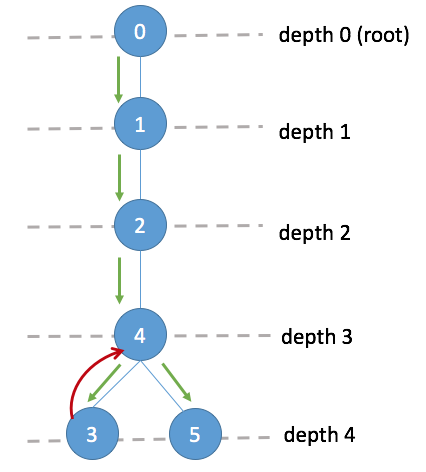
\includegraphics[width=.5\linewidth]{../data_structure/spanning_tree_DFS.png}
\caption{DFS spanning tree for graph depicted in figure \ref{orgkeyword3}.}
\label{orgkeyword4}
\end{figure}

\begin{figure}
\centering
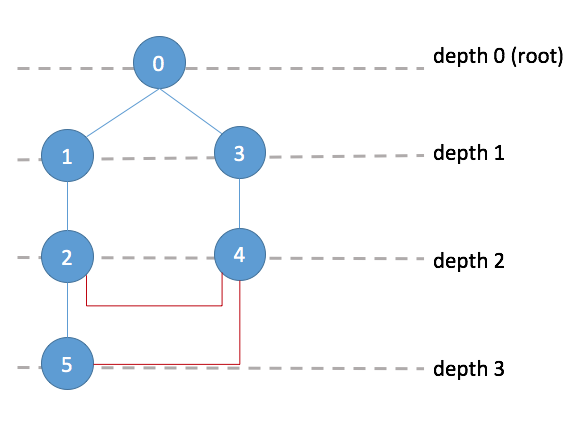
\includegraphics[width=.5\linewidth]{../data_structure/spanning_tree_BFS.png}
\caption{BFS spanning tree for graph depicted in figure \ref{orgkeyword3}.}
\label{orgkeyword5}
\end{figure}



%% \chapter{Codes}
%% \label{sec:orgheadline19}

\subsection{Component-wise Minimum Distance}
\label{sec:orgheadline17}
\begin{lstlisting}[language=C++,frame=single,numbers=none]
  double get_minimum_image_k_from_x(double x, double k, double dimension)
  {
      double kd[3] = {k-dimension - x, k - x, k + dimension - x};
      double re = [get_index_minimum_abs(kd, 3)] + x;
      return re;
  }
\end{lstlisting}

\subsection{DFS for identification of percolation}
\label{sec:orgheadline18}
\begin{lstlisting}[language=python,frame=single, numbers=none]
  def check_travel_beyond_box(pos, index, target, Ld):
      Nd = shape(pos)[1]
     for k in range(Nd):
          if (ident_minimum_distance_k_from_x(pos[index, k], pos[target, k], Ld) != 0):
              return 1
      return 0
  
  def ident_minimum_distance_k_from_x(x, k, box_dimension):
      kd = asarray([k-box_dimension - x, k-x, k+box_dimension-x])
      return argmin(abs(kd)) - 1 # will return [-1, 0, +1]
  
  def ident_over(hash, index, order_count):
      N_cols = shape(hash)[1]
      if order_count >= N_cols:
          return 1
      if int(hash[index, order_count]) is -1:
          return 1
      return 0
  
  def cluster_edge_DFS_travel_restricted_box_iter(hash, pos, Ld, record_component, index=0, order_count=1, cnt=0, IDPC=[], IDPI=[], stack=[], stack_order=[]):
      cnt = 0; const_new_order_count = 1 # initialisation variables
      N_cols = shape(hash)[1] # limitation for the hash tables
      stack.append(int(index)); stack_order.append(order_count) # initial stacking
      while(size(stack) > 0): # will false when size(stack) is 0 if it is not initial step
          cnt += 1 # temporal counting 
          ident_over_cols = ident_over(hash, index, order_count)
          if ident_over_cols: # in the case that the hash[index, order_count] reaching end (-1 or order_count is over)
              stack = stack[:-1]; stack_order = stack_order[:-1]
              if (size(stack) > 0):
                  index = stack[-1]; order_count = stack_order[-1] + 1
          else: # in the case that the hash[index, order_count] is properly defined
              target = hash[index, order_count]
              travel_beyond_box = check_travel_beyond_box(pos, index, target, Ld)
              if (target in record_component) or travel_beyond_box: # when target is in stack stack or travel beyond box boundary
                  if travel_beyond_box: 
                      for id in range(shape(pos[index, :])[0]):
                          ident_IDP = ident_minimum_distance_k_from_x(pos[index, id], pos[target, id], Ld)
                          if (int(ident_IDP) is not 0) and ([index, target] not in IDPI):
                              IDPC.append([id, ident_IDP])
                              IDPI.append([index, target])
                  # when particle is duplicated or travel_beyond_box
                  index = index; order_count = order_count + 1;
  
                  # this means it inherit the exist index for bead but increase order_count
                  # note that the target for next step is given by hash[index, order_count]
              else: # when the target will stack
                  record_component.append(int(target))
                  stack.append(int(target)); stack_order.append(order_count) # record element and its order for stack
                  index = target; order_count = const_new_order_count; # depth first search
      return size(stack)
\end{lstlisting}

  
  
  \chapter{Post-Processing}
  C++ has high performance and various numerical packages has compatible with it. However, it has lack of package to generating graphs, which is crucial point for the purpose of post-processing. On this regards, Python with numpy, scipy, and matplotlib has very flexible and powerful way to measure various quantities and plot it. However, it should be consider that Python is interactive language and even if Python support compiler option, the performance is very slow compared with C++. In addition, there is performance issue with python. Hence, the multiprocess package is used. Since the purpose to use python is easy and simple, the use of multiprocess is not satisfy the purpose. So, except the plotting, if we need to compute with high performance, then it would be better to use C++ package itself. As described on the previous section, the packages are well-integrated and enough supportablility for other post-porcessing except plotting. 

  \section{Stationary State Variable}
  Let $\mathscr{A}$ be a state variable and the system is in equilibrium. That means the $\mathscr{A}$ is fluctuation around a certain average value $A = \langle \mathscr{A}\rangle_t$ when the system is assumed Ergodic. If the sampling time is sufficiently large, the number for time sampling does not affect to the average value, A. In the case of variance, however, it affected by sampling number since we cannot avoid time correlation between two time steps. It is noteworthy that the average value itself said the first moment of $\mathscr{A}$ while the variance is the second moment. On this regards, we can say the time correlation does affect to the moment of $\mathscr{A}$ when the order of moment is higher than 1.

  The easiest way to avoid this problem is to use the sufficiently large time step between data, that means the time steps for statistical processing is higher than the correlation time for the data. There are various method to measure real values, but the box average method is the popular and practically useful \parencite{allen1989computer}.

  \section{Regression Scheme}
  \subsection{Regression by Chebyshev Polynomial}
  Let assumed that the variable $\xi$ is in $[-1, 1]$.
  The generating function for the Chebyshev polynomial is
  \begin{equation}
    \sum_{n=0}^{\infty}T_n(\xi)t^n = \frac{1 - t\xi}{1 - 2t\xi + t^2},
  \end{equation}
  where $T_n$ is n-th order Chebyshev polynomial of the first kind. 
  From it, we can define recursive form:
  \begin{align}
    T_0(\xi) & = 1 \\
    T_1(\xi) & = \xi \\
    T_{n+1}(\xi) & = 2xT_n(\xi) - T_{n-1}(\xi).\label{eq:Chebyshev_recursion}
  \end{align}

  For given analytic function $y = f(\xi)$ where $\xi \in [-1, 1]$, we can expand
  \begin{equation}
    y = \lim_{N\to\infty}\sum_{n=0}^{N} a_nT_n(\xi).\label{eq:Chebyshev_expansion}
  \end{equation}
  Note that typical regression is used for appropriate finite number of $N$ rather than infinite. 

  To compute the coefficient for the equation \eqref{eq:Chebyshev_expansion}, we can define following sum of square error (SSE):
  \begin{equation}
    \chi = \sum_{\alpha=1}^{M} \left[y_\alpha - \sum_{n=0}^{N}a_nT_n(\xi_\alpha)\right]^2,
  \end{equation}
  where $y_\alpha$ denote $\alpha$-th components for given data and $\xi_\alpha$ is its corresponding $\xi$ value.
  This procedure is basically come from the least square method, and directly gave us the normal equation as
  \begin{equation}
    \sum_{k=0}^{N}\left[\sum_{\alpha=1}^{M}T_n(\xi_\alpha)T_k(\xi_\alpha)\right]a_k = \sum_{\alpha=1}^{M}y_{\alpha}T_n(\xi_\alpha)\quad\textrm{for } n\in [0, N].
  \end{equation}
  From this equation, we can define the coefficients, $\mathbf{a} = \{a_1,\cdots,a_M\}$.

  It is noteworthy that even if Chebyshev polynomial is well-known and good basis for regression, analytical handling for the polynomial need some time. In addition, it is equivalent to the Taylor expression with order of $N$, that means we can find the coefficient relation between Chebyshev- and Taylor-style regressions.
  For further detail for the usefulness and properties of Chebyshev polynomial, see the reference \textcite{arfken2008mathematical}.


  \subsection{Typical Polynomial Expression}
  The description on here is following \textcite{SooCho:2013bg} that is practically useful expanation for the regression using Chebyshev polynomial.
  Consider the basic Taylor expansion for $y=f(x)$ with finite order $N$:
  \begin{equation}
    y = \sum_{n=0}^{N} c_n x^n = \sum_{n=0}^{N} b_n\xi^n,
  \end{equation}
  where $\xi$ is scaled x given by
  \begin{equation}
    \xi = \frac{2(x - x_c)}{x_{max} - x_{min}}
  \end{equation}
  with $x_c = \frac{1}{2}(x_{max} + x_{min})$. That is related with the valid region for $\xi$ that defined on the previous section. On this regards, we should find the relation between $\mathbf{a}$ and $\mathbf{b}$.
  Let $T^{(n)}_{k}$ be the n-th order Chebyshev polynomial of the first kind with $k$-th power of $\xi$, from recursive relation for the Chebyshev polynomial, equation \eqref{eq:Chebyshev_recursion}, we have
  \begin{align}
    T_0^{(n+1)} &= -T_0^{(n)} \\
    T_{n+1}^{(n+2)} &= 2T_{n}^{(n+1)} \\
    T_{n+2}^{(n+2)} &= 2T_{n+1}^{(n+1)} \\
    T_k^{(n+2)} &= 2T_{k-1}^{(n+1)}-T_k^{(n)}\quad\textrm{for }1\leq k\leq n,
  \end{align}
  with $T_0^{(0)}=1$, $T_0^{(1)}=0$, and $T_1^{(0)} = 1$. Then we can express $\mathbf{b}$ by $\alpha$ as
  \begin{equation}
    b_n = \sum_{k=n}^{N}T_n^{(k)}a_k,
  \end{equation}
  implies
  \begin{equation}
    c_n = \sum_{k=n}^{N}\left(\frac{2}{\Delta x}\right)^k\left(\begin{array}{c} k \\ n \end{array}\right)\left(-x_c\right)^{k-n}b_k,
  \end{equation}
  where $\Delta x = x_{max} - x_{min}$.
  Finally, we found the coefficients for typical polynomial form
  \begin{equation}
    y = \sum_{n=0}^{N}c_nx^n,
  \end{equation}
  based on Chebyshev polynomial expressions.
  Further details about this connections, see the reference \textcite{SooCho:2013bg}.

  \subsection{Overhead for Recursion}
  It is noteworthy that the given Chebyshev polynomial is generated using recursive relation described on equation \eqref{eq:Chebyshev_recursion}. The recursion is easily implemented into the code by recursive call on function as following python code.

  \begin{lstlisting}[language=Python, frame=single]
    def Chebyshev_1st(n, x): 
    if n==0:
    return 1.0
    elif n==1:
    return x
    return 2.0*x*Chebyshev_1st(n-1, x) - Chebyshev_1st(n-2, x)

    def coe_Chebyshev_1st(k, n): # for coefficient generation
    if k<0 or k > n or (k==0 and n==1):
    return 0
    elif (k==1 and n==1) or (k==0 and n==0):
    return 1
    else:
    return 2*coe_Chebyshev_1st(k-1, n-1) - coe_Chebyshev_1st(k, n-2)
  \end{lstlisting}

  However, it has potential overhead for computing purposes since recursive call for function take time for computing. At the moment, the overhead is ignored because it is only used for post-processing. 


  \section{Empirical Cumulative Distribution}\label{appen_distance_distribution}
  Distance distribution function is of importance to identify the system properties because the given integrator cannot be specify the velocity of each particles. The empirical cumulative distribution is simply calculated by sorting method. Let $Y$ be data column that related with random generation. To make sort $Y$ column then making index for $Y$ related with its population rate to increase. This is exactly the same with the definition for the cumulative distribution that we are using for. For given cumulative distribution, $\mathscr{F}(r)$, we can define probability distribution function, $P(r)$, as
  \begin{equation}
    P(r) = \frac{d}{dr}\mathscr{F}(r).
  \end{equation}

  It is of importance that the CDF on this scheme has irregular X-axis, that is the $dx_i = x_i - x_{i-1}$ has different values while $dy_i = y_i - y_{i-1}$ has constant values, which make difficulty to use regression along the CDF. Hence, the two-scheme is involved for both of interpolation and derivation for short interval and compared with the results. Typically, the piece-wise cubic spline is involved all area, even if it is highly fluctuating, in order to use reference for trend. Then, the fitted curve will be compared with this reference.

  
  \section{Plotting and Making Movie for Trajectory File}
  In this case, get appropriate marker size for beads is of importance in order to recognize the effective range for the system. Typically, transform package in matplotlib is used for this aspect.
  \begin{lstlisting}[language=Python,frame=single,numbers=none]
    marker_unit = (ax.transData.transform((1, 0)) - ax.transData.transform((0, 0)))[0]
  \end{lstlisting}

  Since the given trajectory file is quite big, loading all the fild into the memory has potential problems. It is of importance to get line-by-line rather than loadtxt functionality of numpy package because loadtxt load all file into memory at once. Note that parsing each file line had overhead compared with the loadtxt functionality. Hence, for smaller files, it prefer to use the loadtxt. From line parsing, we can allowed to use parallel computing. For the author's point of view, using GNU's terminal tool parallel is good for various aspect. In this case, however, the data file can be big enough to overflow memory and it is the reason to choose parsing data, directly, rather than using loadtxt. On this regards, multiprocess package in Python is selected. For this integrate, the following main function should be developed. Note that number of processes is set by given value, N{\_}proc, that can be 'None' variable. Then, the multiprocess package automatically allocate one thread for each logical processor. The ``partial'' package is loaded because the allocation of multiprocess does not taking various arguments, so the package allow to transfer more argument that might be needed for the plotting function.

  \begin{lstlisting}[language=Python,frame=single]
    from multiprocessing import Pool
    from functools import partial

    def plot_t(given_traj, t):
    # statement (detail for plot_t is omitted)

    if __name__ == '__main__':
    pool = Pool(processes=N_proc)
    with open(fn, 'r') as f:
    N_cols = 2*N_dimension*Np + 1
    tmp_arr = zeros([N_proc, N_cols])
    cnt_line = 0
    c_t = arange(N_proc)
    for line in f:
    tmp_str = line.split('\t')
    for i in range(N_cols):
    tmp_arr[cnt_line%N_proc, i] = float(tmp_str[i])
      cnt_line += 1
      if (cnt_line <> 0 and cnt_line%N_proc == 0):
      pool.map(partial(plot_t, tmp_arr), c_t)
      c_t += N_proc
  \end{lstlisting}

  Finally, we have all the figure with proper image file format. In this processing, author is prefer to use png format rather than pdf since it need for ffmepg incoding. The basic statement for ffmpeg is used as follow. But, codec, output file, and various properties can be set with the ffmpeg package. For instance, h268 codec is useful for Mac compatible movie.
  \begin{lstlisting}[frame=single,numbers=none]
    ffmpeg -i t%08d.png -vcodec copy out.mov
  \end{lstlisting}

  \section{Trajectory Conversion}\label{appen_traj_conv}
  Since the simulation is using periodic boundary condition (PBC), all the trajectory is already cut inside of certain box. For some reasons of post-processing, MSD and so on, we need to recover from PBC image to real beads trajectory. This conversion is easily doable with appropriate condition for the identity for trajectory. Here, I have used half of box dimension is changed from the previous output step, the trajectory is identified as jump and post-processing code will recover it. Note that the trajectory output frequency is lower than the all time steps, if this conversion is needed, we have to reduce the overall time steps. The core parts of the code is listing as below. 
  \begin{lstlisting}[language=Python, frame=single]
    def sign(x):
    if x < 0.:
    return -1.
    return 1.

    def inv_PBC(x_now, x_next, LB):
    dX = x_next - x_now
    if abs(dX) > 0.5*LB:
    return inv_PBC(x_now, x_next - sign(dX)*LB, LB)
    return x_next

    for i in range(NP):
    for k in range(ND):
    index_Rik = 2*ND*i + 1 + k
    for t in range(1, Nt):
    dat[t, index_Rik] = inv_PBC(dat[t-1, index_Rik], dat[t, index_Rik], LB)
  \end{lstlisting}
  Note that the inverse mapping function, inv{\_}PBC, is using recursive call, that is because the main process override the opened dat array for effienciency issue, that sometimes amplified the existing gap during correction. Therefore, it is of importance to check the range is valid for inverse mapping using recursive call.
  From this conversion, we can easily expect the trajectory from figure \ref{fig:traj_conv}. Note that the judgment is based on the half of box dimension. 
  \begin{figure}
    \centering
    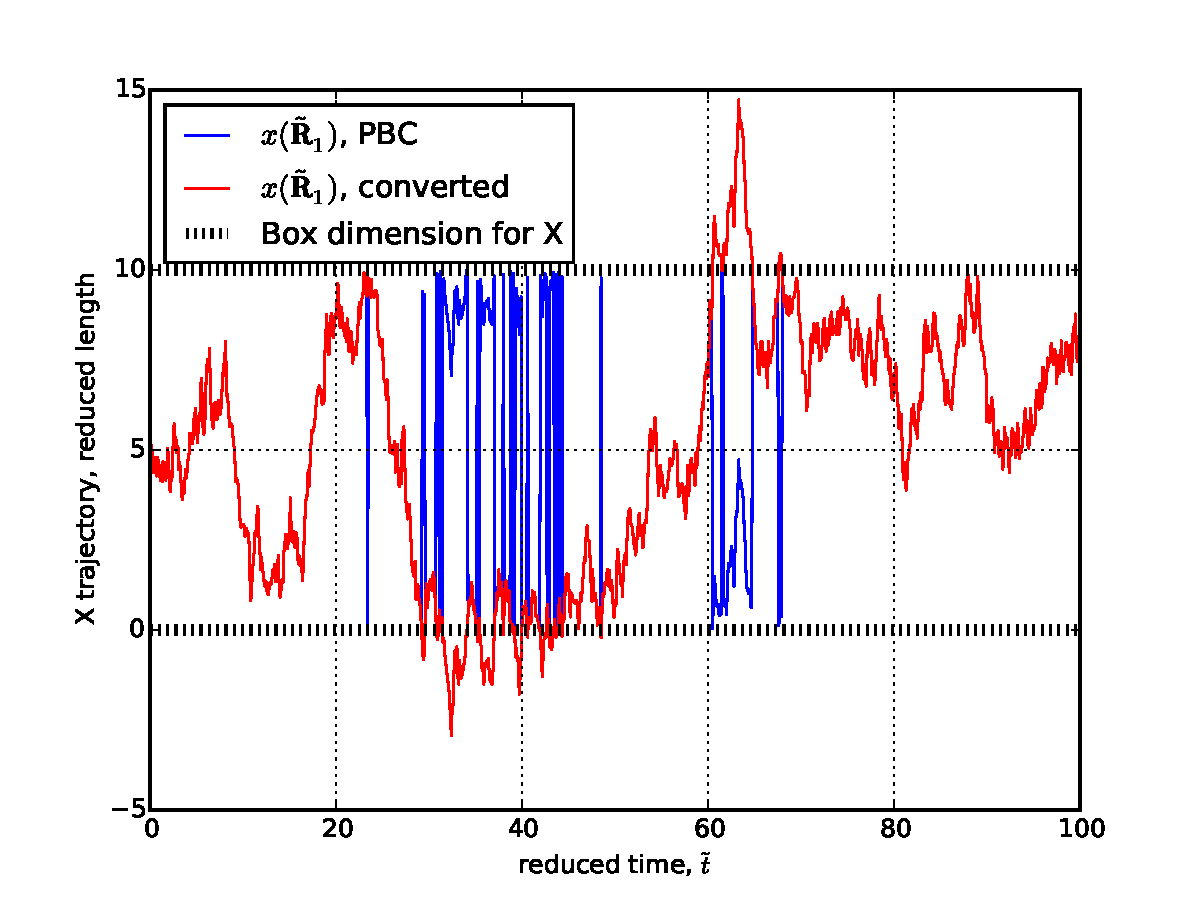
\includegraphics[width=\textwidth]{figures/converting_trajectory.pdf}
    \caption{Test results for trajectory conversion. Blue color represent the trajectory using periodic boundary condition (PBC) and the red color represent the converted data. The test is done using pure Brownian motion with 100 reduced time step, and trajectory is involved only for x-coordinate of the first beads among 100 beads on the system.}
    \label{fig:traj_conv}
  \end{figure}

  % \section{Radial Distributon Function}
  % By definition, the radial distribution function is given by
  % \begin{equation}
  %   \rho g(\mathbf{r})d\mathbf{r} = dn(\mathbf{r}) = \langle \sum_{i\neq 0}\delta(\mathbf{r}-\mathbf{r}_i\rangle_t d\mathbf{r}
  % \end{equation}
  % where $\rho$ is density of system. 
  \section{Pair Correlation Function}
  \label{appen_rdf}
  \subsection{Theoretical Background}
  The pair correlation distribution, $\rho(\mathbf{r}_1, \mathbf{r}_2$, is one of the important distribution function to show the structure information. There are various relation exist with spatial or reciprocal information.

  For given canonical ensemble $(N, V, T)$, let $Z$ be configurational integral, partition function:
  \begin{equation}
    Z = \int d\boldsymbol{\Gamma}_{1}^{N} \exp\left(-\beta U(\boldsymbol{\Gamma}_{1}^{N})\right),
  \end{equation}
  where $\beta$ be Boltzmann factor, $\boldsymbol{\Gamma}_{1}^{N} = \{\mathbf{r}_1,\cdots,\mathbf{r}_N\}$ and $d\boldsymbol{\Gamma}_{1}^{N} = d\mathbf{r}_1\cdots d\mathbf{r}_N$. Then, the probability of an elementary configuration is expressed by
  \begin{equation}
    P(\boldsymbol{\Gamma}_{1}^{N})d\boldsymbol{\Gamma}_{1}^{N} = \frac{\exp\left(-\beta U(\boldsymbol{\Gamma}_{1}^{N})\right)}{Z}d\boldsymbol{\Gamma}_{1}^{N},
  \end{equation}
  where $d\boldsymbol{\Gamma}_{1}^{N} = d\mathbf{r}_1\cdots d\mathbf{r}_N$.
  Let $P(\boldsymbol{\Gamma}_{1}^{N})$ be configurational distribution over set of N-number of state variables, $\boldsymbol{\Gamma}_{1}^{N} = \{\mathbf{r}_1, \cdots, \mathbf{r}_N\}$. Since the configurational distribution $P(\boldsymbol{\Gamma}_{1}^{N})$, is function of potential energy, $U(\boldsymbol{\Gamma}_{1}^{N})$, it cannot account only for single particle. Hence, we can eliminating dependency of other particles using integrate over configurational space:
  \begin{equation}
    P(\boldsymbol{\Gamma}_{1}^{n}) = \int d\boldsymbol{\Gamma}_{n+1}^{N} P(\boldsymbol{\Gamma}_{1}^{N}),
    \label{eq:reduced_configuration_distribution}
  \end{equation}
  which is joint PDF for finding particle $\{1, 2, \cdots, n\}$ at $\{\mathbf{r}_1, \mathbf{r}_2, \cdots, \mathbf{r}_n\}$, respectively. It is called \textit{specific} PDF because of the index of particles are fixed.
  Let $\boldsymbol{\Omega}_{1}^{n} = \{\mathbf{r}_1,\cdots,\mathbf{r}_n\}$ be the set of particles which is arbitrarily chosen.
  If the particles are identical (indistinguishable system), we can express \textit{generic} PDF when we allow to choose particles, arbitrarily:
  \begin{equation}
    \rho(\boldsymbol{\Omega}_{1}^{n}) = \frac{N!}{(N-n)!}P(\boldsymbol{\Gamma}_{1}^{n})\label{eq:generic_PDF}
  \end{equation}
  % Again, the LHS of Eq. \eqref{eq:generic_PDF} is not specified for particles index while the RHS is specified for particles.
  For simplification, consider the given material is isotropic. Then the first order generic PDF becomes its density: $\rho(\mathbf{r}_1) = \rho = N/V$. When the particles independent to each other, the joint probability becomes 
  \begin{equation}
    P_{id}(\boldsymbol{\Gamma}_{1}^{N}) = \prod_{k=1}^{N}P(\mathbf{r}_k) = \rho^{N}.\label{eq:independent_PDF}
  \end{equation}
  Therefore, the generic PDF for independent particle becomes
  \begin{equation}
    \rho_{id}(\boldsymbol{\Omega}_{1}^{n}) = \frac{N!}{(N-n)!}P(\boldsymbol{\Gamma}_{1}^{n}) = \frac{N!}{(N-n)!}\rho^n.
  \end{equation}
  The correlation function $g$ is given by the fraction of generic PDF of the system to the independent case:
  \begin{equation}
    g(\boldsymbol{\Omega}_{1}^{n}) \equiv \frac{\rho(\boldsymbol{\Omega}_{1}^{n})}{\rho_{id}(\boldsymbol{\Omega}_{1}^{n})} = \frac{P(\boldsymbol{\Gamma}_{1}^{n})}{P_{id}(\boldsymbol{\Gamma}_{1}^{n})}=\frac{1}{\rho^n}P(\boldsymbol{\Gamma}_{1}^{n}).
  \end{equation}
  For convenience, $h(\boldsymbol{\Omega}) = g(\boldsymbol{\Omega}) - 1$ is frequently used as correlation function.
  Inversely, we have \textit{specific} PDF:
  \begin{equation}
    P(\boldsymbol{\Gamma}_{1}^{n}) = \rho^n g(\boldsymbol{\Omega}_{1}^{n}).
  \end{equation}
  When order is 2, the correlation functions is called pair correlation function:
  \begin{align}
    g(\mathbf{r}_1, \mathbf{r}_2) &= \frac{1}{\rho^2}P(\mathbf{r}_1, \mathbf{r}_2) = \frac{1}{\rho^2}\int d\boldsymbol{\Gamma}_{3}^{N}P(\mathbf{r}_1, \mathbf{r}_2) \\
    &= \frac{1}{\rho^2}\int d\boldsymbol{\Gamma}_{3}^{N} \frac{\exp(-\beta U(\boldsymbol{\Gamma}_{1}^{N}))}{Z}.
  \end{align}
  For spherically symmetric system, the probability between $\mathbf{r}_i$ and $\mathbf{r}_j$ becomes
  \begin{equation}
    P(\mathbf{r}_i, \mathbf{r}_j) = P(\mathbf{r}_i - \mathbf{r}_j).
  \end{equation}
  For further details, see \textcite{chandler1987}.


  \subsection{Measuring from Simulation Data}
  Let $\langle n_i(r, \Delta r; t)\rangle_t$ be the average number in the shell at distance between $r$ and $r+\Delta r$ at time t: 
  \begin{equation}
    \langle n_i(r, \Delta r; t)\rangle_t = \frac{1}{T}\sum_{j=1}^{T}n_{i}(r;t_j).
  \end{equation}
  Note that $\langle n_i(r)\rangle$ is independent on $i$, then we can define ensemble average of number of particles as
  \begin{equation}
    \langle n(r, \Delta r; t)\rangle \equiv \frac{1}{N}\sum_{i=1}^{N}\frac{1}{T}\sum_{j=1}^{T}n_{i}(r, \Delta r; t_j).
  \end{equation}
  Let assumed the particles are uncorrelated, the same assumption of independent probability between particles in equation \eqref{eq:independent_PDF}, then we averaged number in the shell at distance $r$:
  \begin{equation}
    \langle n(r, \Delta r)\rangle_{unc} = \rho V(r, \Delta r) (N-1)/N,
  \end{equation}
  where $V(r, \Delta r)$ is Volume of shell between $r$ and $r+\Delta r$, and $\rho$ is density.
  The alternative form of radial distribution function is the ratio between averaged number of particles on shell with distance $r$ and the uncorrelated number:
  \begin{align}
    g(r) &= \frac{\langle n(r, \Delta r; t)\rangle}{\langle n(r, \Delta r)\rangle_{unc}} \\
    &= \frac{1}{\rho V(r, \Delta r)(N-1)T}\sum_{i=1}^{N}\sum_{j=1}^{T}n_i(r, \Delta r; t_j).\label{eq:practical_RDF}
  \end{align}
  If the given material is liquid-like and is not highly ordered case, the averaged number at long distance becomes un-correlated averaged number:
  \begin{equation}
    \lim_{r\to\infty} g(r) = \frac{\lim_{r\to\infty}\langle n(r,\Delta r;t)\rangle}{\langle n(r,\Delta r)\rangle_{unc}} = \frac{\langle n(r,\Delta r)\rangle_{unc}}{\langle n(r,\Delta r)\rangle_{unc}} = 1.
  \end{equation}
  Because of system size, the density $\rho$ should be replaced by local density, i.e., the counted number for all the particles divided by total area that is considered:
  \begin{equation}
    \rho_{D} = \frac{1}{T(N-1)V_D}\sum_{k=1}^{N-1}\langle n(r, \Delta r;t)\rangle \equiv \frac{n_D}{T(N-1)V_D},
  \end{equation}
  where subscript $D$ denote domain of computation. 
  For simplification, let $\rho(r)$ be the averaged density between $r$ and $r+\Delta r$:
  \begin{equation}
    \rho(r) = \frac{\langle n(r, \Delta r; t)\rangle}{V(r, \Delta r)}. % = \frac{1}{V(r,\Delta r)NT}\sum_{i=1}^{N}\sum_{j=1}^{T}n_i(r,\Delta r;t_j). 
  \end{equation}
  Note that $\rho(r)$ is not affected by $\Delta r$ since the counted number for histogram directly proportional to the volume: $\langle n(r, \Delta r; t)\rangle \propto V(r, \Delta r)$.
  The equation \eqref{eq:practical_RDF} becomes
  \begin{equation}
    g(r) = \frac{\rho(r, \Delta r)}{\rho_D} = \frac{V_D}{n_D}\frac{\langle n(r, \Delta r; t)\rangle}{V(r, \Delta r)}, \label{eq:practical_RDF_refine}
  \end{equation}
  which is the same formular compared with GROMACS.
  

  For practical purpose, the pairs are only accounted for once rather than twice. On this regards, the $N-1$ factors replaced by $(N-1)/2$ which reduced the time consumption dramatically. 
  \begin{lstlisting}[language=Python,frame=single]
def get_ddf(traj, ts, Np, N_dimension, box_dimension, cut_ratio):
    ddf = []
    for t in ts:
        for i in range(Np-1):
            for j in range(i+1, Np):
                d = lin.norm(get_rel_vec(traj, t, i, j, N_dimension, box_dimension))
                if d<cut_ratio*box_dimension:
                    ddf.append(d)
    return ddf

def get_rdf_ref(traj, ts, dr, Np, N_dimension, box_dimension, cut_ratio):
    Nr = int(cut_ratio*box_dimension/dr)
    rdf = zeros([Nr, 3])
    rdf[:,0] = arange(0, cut_ratio*box_dimension, dr)
    ddf = get_ddf(traj, ts, Np, N_dimension, box_dimension, cut_ratio)
    N_tot = size(ddf)
    Nt = size(ts)
    for r in ddf:
        rdf[int(r/dr), 1] += 1
    if (N_dimension == 3):
        Vr = (4./3.)*pi*((rdf[:,0]+dr)**3.0 - rdf[:,0]**3.0)
        Vrmax = (4./3.)*pi*(cut_ratio*box_dimension)**3.0
        rho_local = N_tot/(Nt*0.5*(Np-1)*Vrmax)
    elif (N_dimension == 2):
        Vr = pi*((rdf[:,0]+dr)**2.0 - rdf[:,0]**2.0)
        Vrmax = pi*(cut_ratio*box_dimension)**2.0
        rho_local = N_tot/(Nt*0.5*(Np-1)*Vrmax)
    print 'rho_local = ', rho_local
    rdf[:,2] = rdf[:,1]/(Vr*0.5*(Np-1)*Nt*rho_local)
    rdf[0, 2] = 0. 
    return rdf
    \end{lstlisting}
    The cut-ratio typically set by half of box dimension because of computing efficiency. When this is half box dimension, we can apply minimum image convention easily. If it is larger than half of box dimension, we have to checked all the possible map for counting. If it is smaller than half of box dimension, we loose some information which is meaningful for us. 
    The results is described on figure \ref{fig:rdf_exam} which is used the code reported on here. 


    \begin{figure}
      \centering
      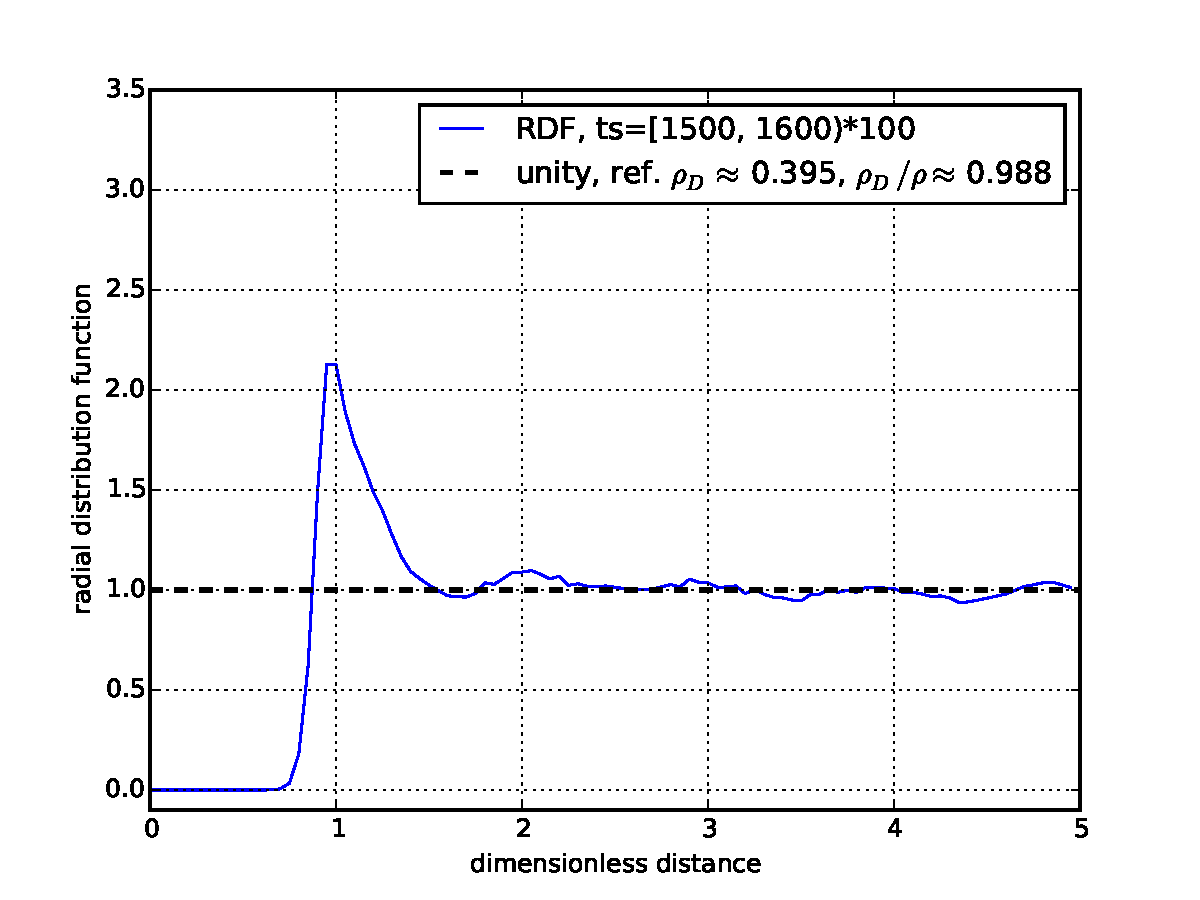
\includegraphics[width=\textwidth]{figures/rdf_exam.pdf}\\
      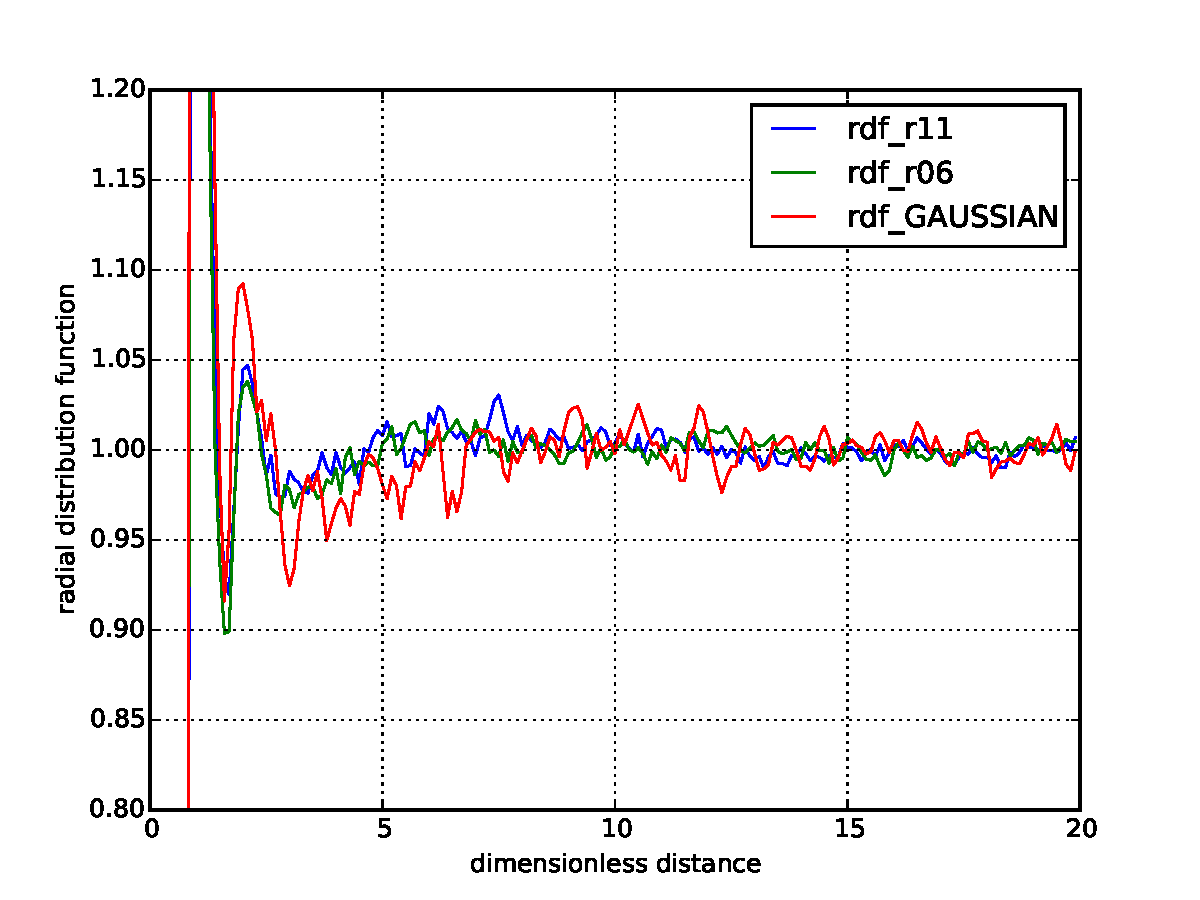
\includegraphics[width=\textwidth]{figures/rdf_compare.pdf}
      \caption{Radial distribution function for NP640/1600AREA example. Time average is applied over 100 times steps. Upper case is simple time average for FENE with $R_m/R_0$ ratio 11. The lower case is the comparison between FENE ratio 11 and 6 with Gaussian (red color) case.}
      \label{fig:rdf_exam}
    \end{figure}
    
    \section{Structure Factor}
    \subsection{Basics}
    The basic definition for the structure factor is given by
    \begin{equation}
      S(\mathbf{k}) = N^{-1}\left\langle \sum_{i,j=1}^{N}\exp\left[i\mathbf{k}\cdot(\mathbf{r}_i - \mathbf{r}_j)\right] \right\rangle\quad\textrm{for }\mathbf{r}_i,\mathbf{r}_j\in\boldsymbol{\Gamma}_{1}^{N},
    \end{equation}
    where $\mathbf{k}$ is wave vector. The given formula can be analyzed by two parts:
    \begin{align}
      S(\mathbf{k}) &= N^{-1}\left\langle \sum_{i,j}\delta_{ij}\right\rangle + N^{-1}\left\langle \sum_{i, j\neq i}\exp(i\mathbf{k}\cdot(\mathbf{r}_i - \mathbf{r}_j))\right\rangle \\
                    &= 1 + N^{-1}\sum_{i,j\neq i}\frac{1}{Z}\int d\boldsymbol{\Gamma}_{1}^{N}\exp(-\beta U(\boldsymbol{\Gamma}_{1}^{N}))\exp(i\mathbf{k}\cdot(\mathbf{r}_i-\mathbf{r}_j))\\
                    &= 1 + N^{-1}\sum_{i, j\neq i}\int d\mathbf{r}_i d\mathbf{r}_j\left[\exp(i\mathbf{k}\cdot(\mathbf{r}_i-\mathbf{r}_j)) \int d\left(\boldsymbol{\Gamma}_{1}^{N}\backslash\{\mathbf{r}_i,\mathbf{r}_j\}\right)\frac{\exp(-\beta U(\boldsymbol{\Gamma}_{1}^{N}))}{Z}\right]\\
                    &= 1 + N^{-1}\sum_{i,j\neq i}\int d\mathbf{r}_i d\mathbf{r}_j P(\mathbf{r}_i, \mathbf{r}_j) \exp(i\mathbf{k}\cdot(\mathbf{r}_i - \mathbf{r}_j)).
    \end{align}
    Let assumed that the system is spherically symmetry, then the probabilty $P(\mathbf{r}_i, \mathbf{r}_j)$ becomes the probability for its relative vector, $P(\mathbf{r}_i-\mathbf{r}_j)$, which implies
    \begin{align}
      S(\mathbf{k}) &= 1 + N^{-1}\sum_{i,j\neq i}\int d\mathbf{r}_i d\mathbf{r}_j P(\mathbf{r}_i - \mathbf{r}_j)\exp(i\mathbf{k}\cdot(\mathbf{r}_i - \mathbf{r}_j)) \\
      &= 1 + N^{-1}\sum_{i,j\neq i}\int d\mathbf{r}_i d\mathbf{r}_j  \mathscr{F}\left[P(\mathbf{r})\delta(\mathbf{r} - (\mathbf{r}_i - \mathbf{r}_j)) \right] \\
      &= 1 + N^{-1}\mathscr{F}\left[P(\mathbf{r}) \sum_{i,j\neq i}\int d\mathbf{r}_i d\mathbf{r}_j \delta(\mathbf{r} - (\mathbf{r}_i - \mathbf{r}_j)) \right],
    \end{align}
    where $\mathscr{F}$ denote spatial Fourier transform:
    \begin{equation}
      \mathscr{F}[f(\mathbf{r})] = \int d\mathbf{r} f(\mathbf{r})\exp(i\mathbf{k}\cdot\mathbf{r}).
    \end{equation}
    The integration part becomes
    \begin{align}
      \int d\mathbf{r}_i d\mathbf{r}_j \delta(\mathbf{r} - (\mathbf{r}_i - \mathbf{r}_j)) &= \int d\mathbf{r}_i d\mathbf{r}_{ij} \delta(\mathbf{r} - \mathbf{r}_{ij}) \\
      &= \int d\mathbf{r}_i 1
    \end{align}
    \textbf{Derivation is on-going}
    \subsection{Related with Radial Distribution Function, 3D}
    \begin{equation}
      S(\mathbf{q}) = 1 + \rho\mathscr{F}\left[g(\mathbf{r}) - 1\right],
    \end{equation}
    where $g(\mathbf{r})$ is given radial distribution function with respect to distance vector, $\mathbf{r}$, and $\mathscr{F}$ is Fourier transform from spatial vector, $\mathbf{r}$, to the its reciprocal (wave) vector, $\mathbf{q}$. Therefore, the structure factor becomes
    \begin{equation}
      S(\mathbf{q}) = 1 + \rho \int d\mathbf{r}\, e^{i\mathbf{q}\cdot\mathbf{r}}\left[g(\mathbf{r}) - 1\right].
    \end{equation}
    For isotropic system (orientational symmetric), the integration part becomes further simple. For simplification, let assumed that the direction of axis x is the same with the given wave vector, $\mathbf{q}$:
    \begin{align}
      S(q) &= 1 + \rho \int r^2\sin\theta \,dr d\theta d\phi\, \exp(iqr\cos\theta)(g(r) - 1)  \nonumber\\
           &= 1 + 2\pi\rho \int dr \,r^2(g(r) - 1) \int_0^{\pi} d\theta \,\sin\theta\exp\left(iqr\cos\theta\right) \nonumber\\
           &= 1 + 2\pi \rho \int dr \,r^2(g(r) - 1) \int_{-1}^{1}dt \,\exp(iqrt) \nonumber\\
           &= 1 + 2\pi \rho \int dr \,r^2(g(r) - 1) \frac{\exp(iqr)-\exp(-iqr)}{iqr} \nonumber\\
           &= 1 + 2\pi \rho \int dr \,r^2(g(r) - 1) \frac{2}{qr}\sin(qr), \quad(\because\textrm{Euler's equation})\nonumber\\
           &= 1 + 4\pi \frac{\rho}{q} \int dr \,r\sin(qr)(g(r) - 1).
    \end{align}

    \subsection{Isotropic Structure Factor for 2 Dimensional Case}

 Similar to the 3-dimensional case, the axis is tuned with the given wave vector, $\mathbf{q}$. Then we have
    \begin{equation}
      S(q) = 1 + \rho \int r\,drd\theta\, \exp(iqr \cos\theta)(g(r) - 1).
    \end{equation}
    Here, the integration of $\exp(iqr \cos\theta)$ over angle $\theta$ does not shows the closed form, but we can express it as 0-th order of Bessel function of the first kinds:
    \begin{equation}
      2\pi J_0(x) = \int_{0}^{2\pi}d\theta\, \exp(ix\sin\theta) = \int_{0}^{2\pi}d\theta\, \exp(ix\cos\theta),
    \end{equation}
    where general Bessel function is possibly expressed by trigonometric functions:
    \begin{align}
      \pi J_n(x) &= \int_0^{\pi}d\theta\,\cos(x\sin\theta)\cos (n\theta) , \quad\textrm{n is even} \\
      \pi J_n(x) &= \int_0^{\pi}d\theta\,\sin(x \sin\theta)\sin (n\theta) , \quad\textrm{n is odd}.
    \end{align}
    For further details, see \textcite{arfken2008mathematical}.
    On this regards, the isotropic structure factor for 2-dimensional case is expressed by
    \begin{equation}
      S(q) = 1 + 2\pi \rho \int dr \,r J_0(qr) (g(r) - 1),
    \end{equation}
    which cannot be solved by analytically. 
    The given $J_0(qr)$ is oscillatory decreasing function with respect to $qr$ (reported in figure \ref{fig:iso_av_orientation}) but $rJ_0(qr)$ is oscillatory increasing function. Therefore, $g(r)-1$ should be conversed to zero faster than that of $rJ_0(qr)$. 

    \begin{figure}
      \centering
      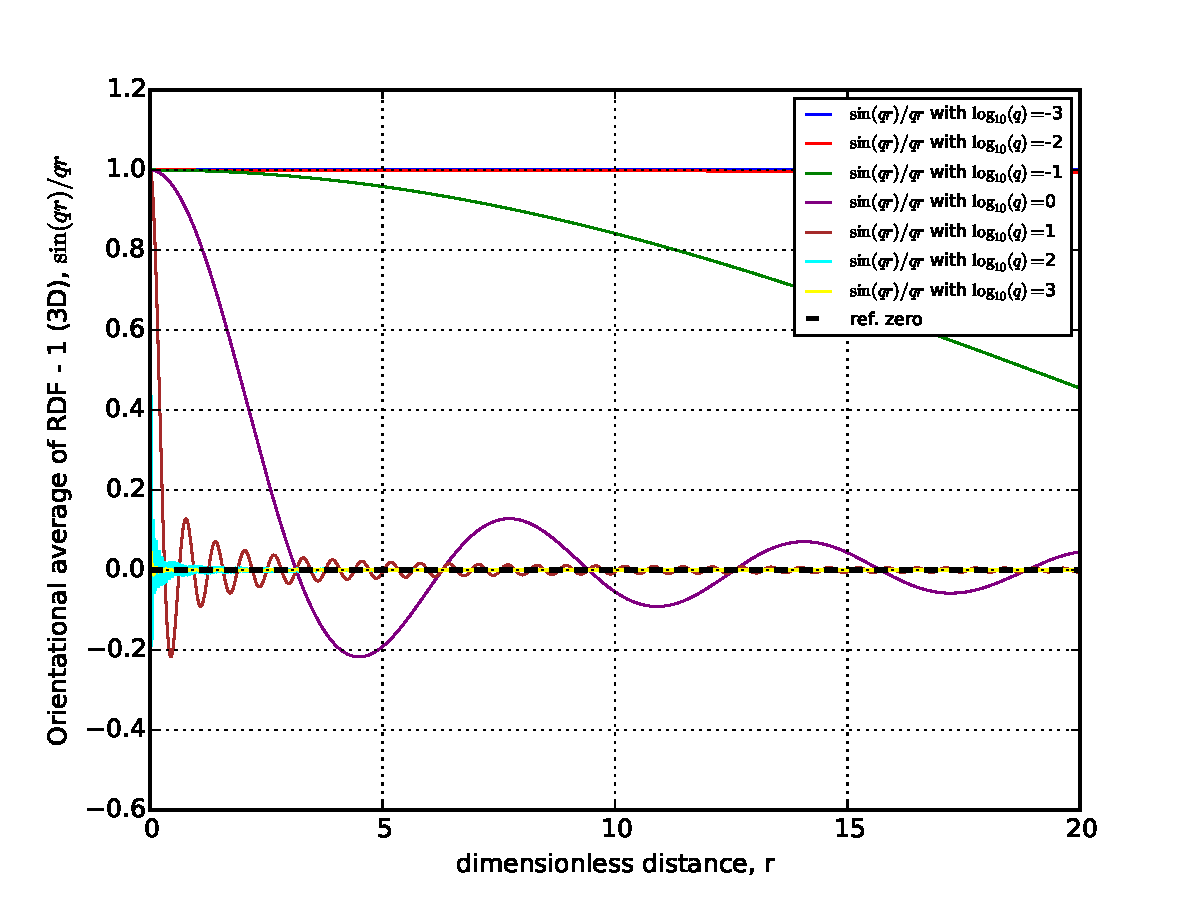
\includegraphics[width=0.9\textwidth]{figures/kernel.pdf}\\
      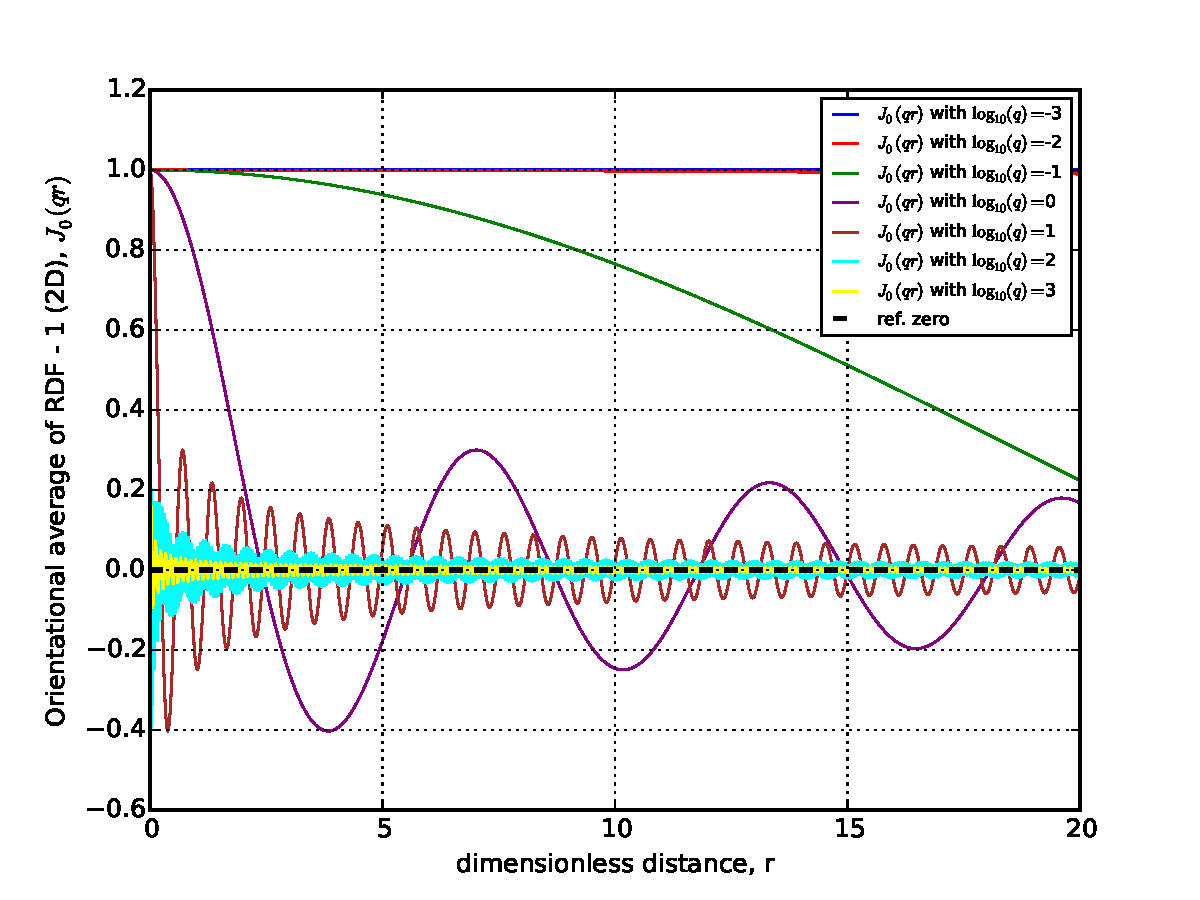
\includegraphics[width=0.9\textwidth]{figures/J_0_qr.pdf}
      \caption{Orientational average over $g(r)-1$ in 3-dimensional (up) and 2-dimensional (down) cases. The upper case is related with the Debye equation while the lower case is expressed by the zeroth order of Bessel function with the first kind.}
      \label{fig:iso_av_orientation}
    \end{figure}

    %% \begin{figure}
    %%   \centering
    %%   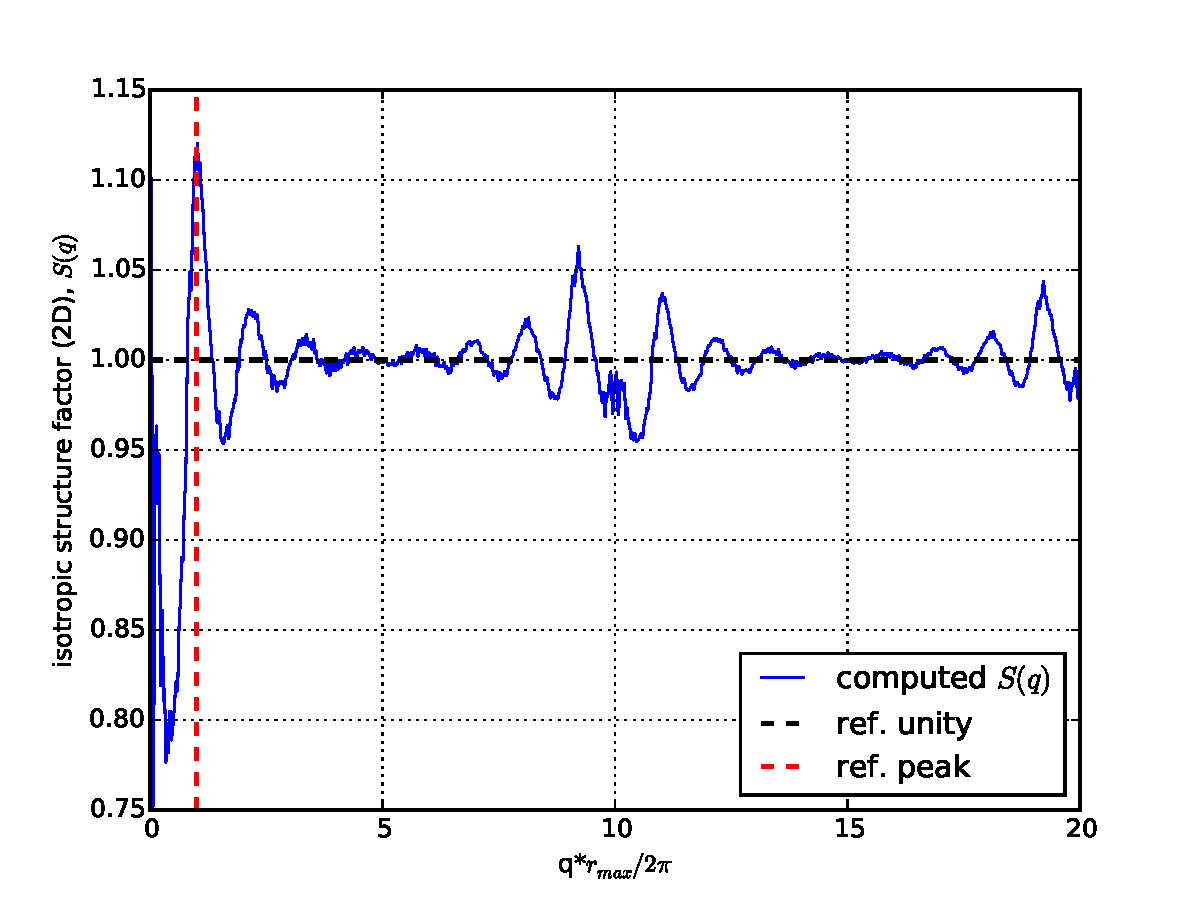
\includegraphics[width=\textwidth]{figures/FENE_r11_Sq_linear.pdf}\\
    %%   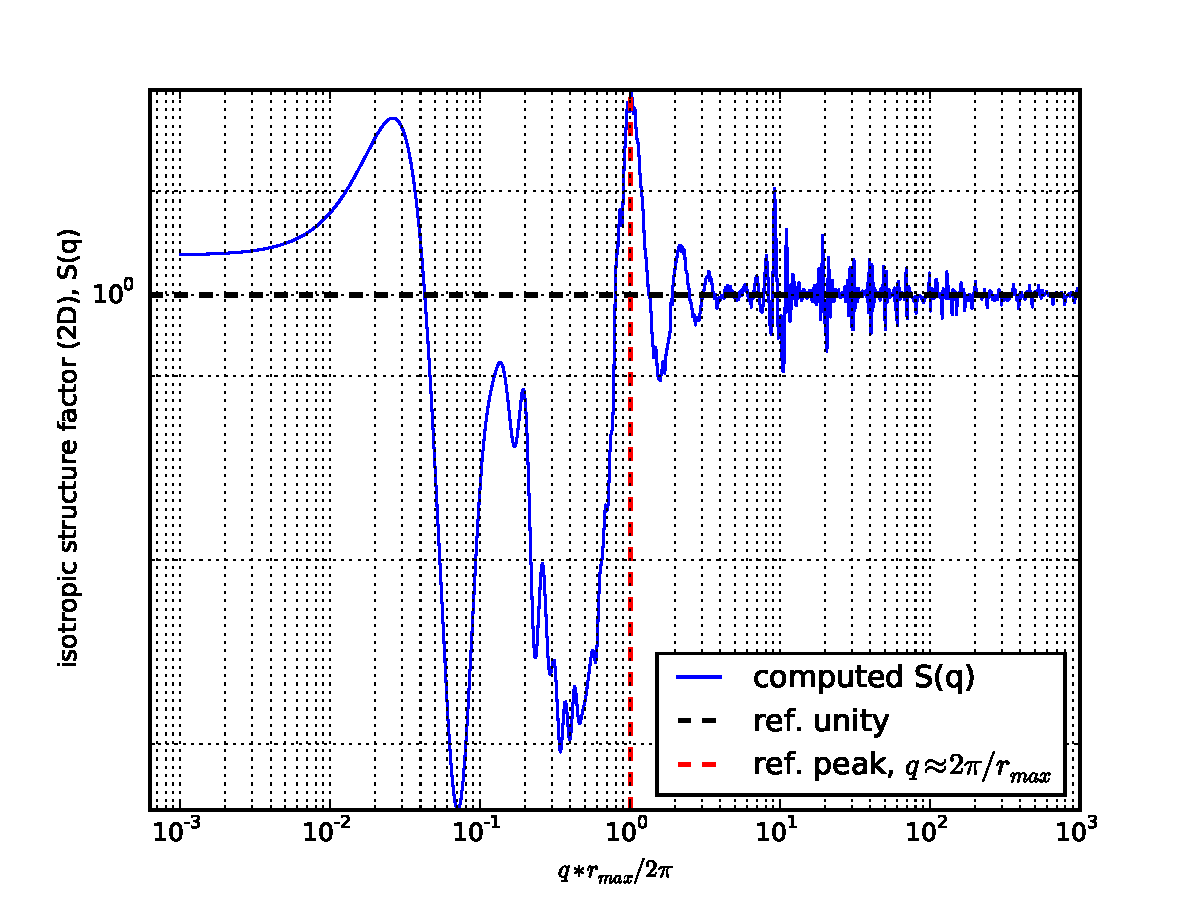
\includegraphics[width=\textwidth]{figures/FENE_r11_Sq_log.pdf}
    %%   \caption{Results of FENE with ratio $R_M/R_0=11$. The given radial distribution is exactly the same with figure \ref{fig:rdf_exam} (lower case). The upper case is computed structure factor in linear scale, and the bottom is the double log scales for the structure factor.}
    %%   \label{fig:2d_Sq}
    %% \end{figure}

    %% \begin{figure}
    %%   \centering
    %%   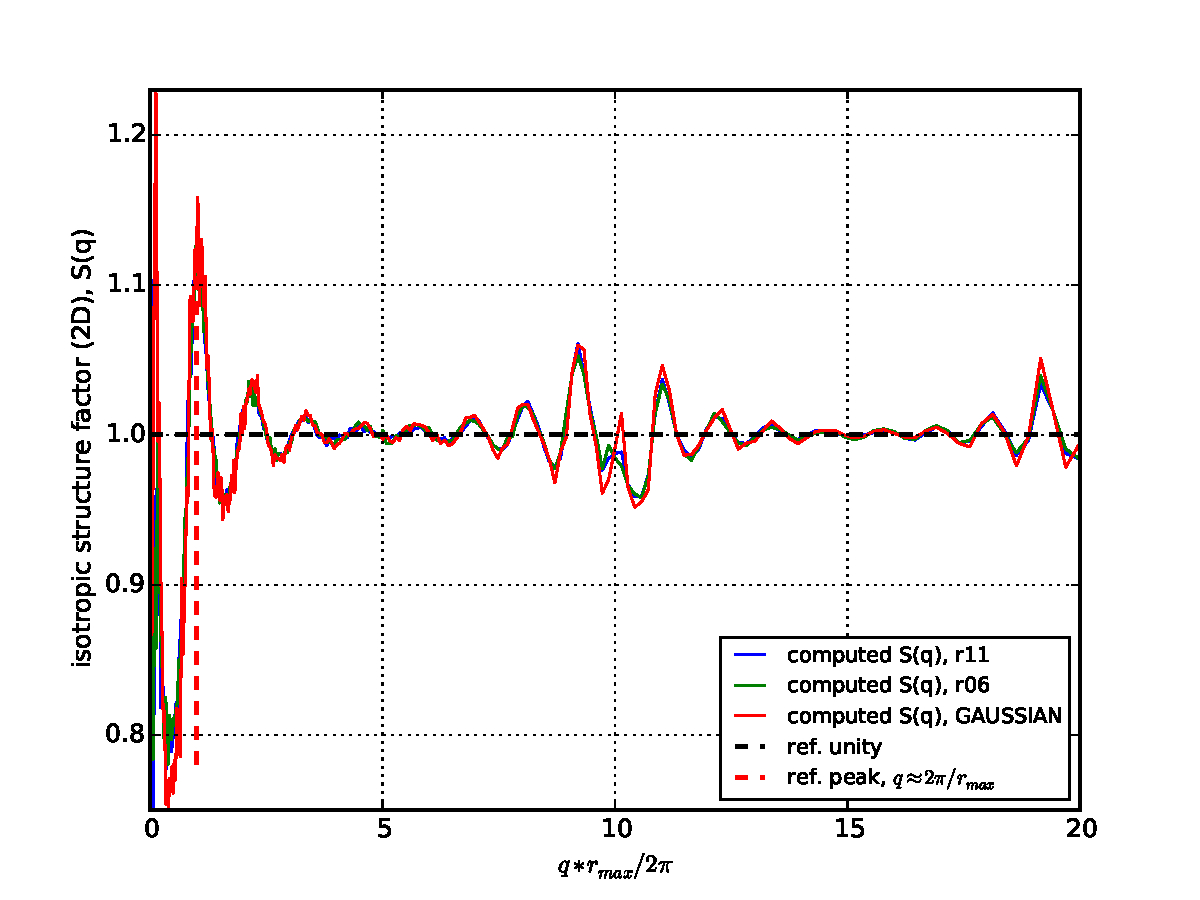
\includegraphics[width=\textwidth]{figures/Sq_compare_linear.pdf}\\
    %%   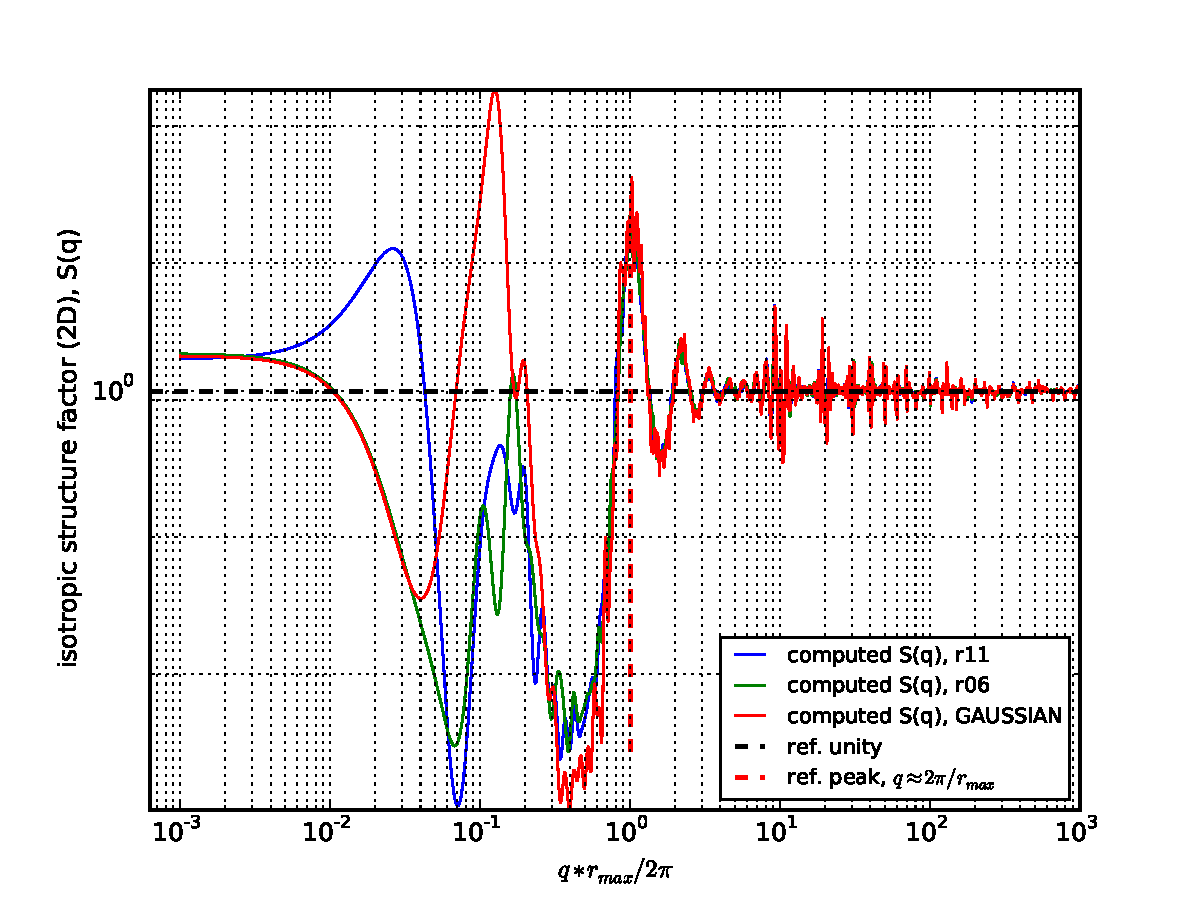
\includegraphics[width=\textwidth]{figures/Sq_compare_log.pdf}
    %%   \caption{Results with different FENE ratio and GAUSSIAN. The given radial distribution is exactly the same with figure \ref{fig:rdf_exam} (lower case). The upper case is computed structure factor in linear scale, and the bottom is the double log scales for the structure factor.}
    %%   \label{fig:2d_Sq_compare}
    %% \end{figure}

    \begin{figure}
      \centering
      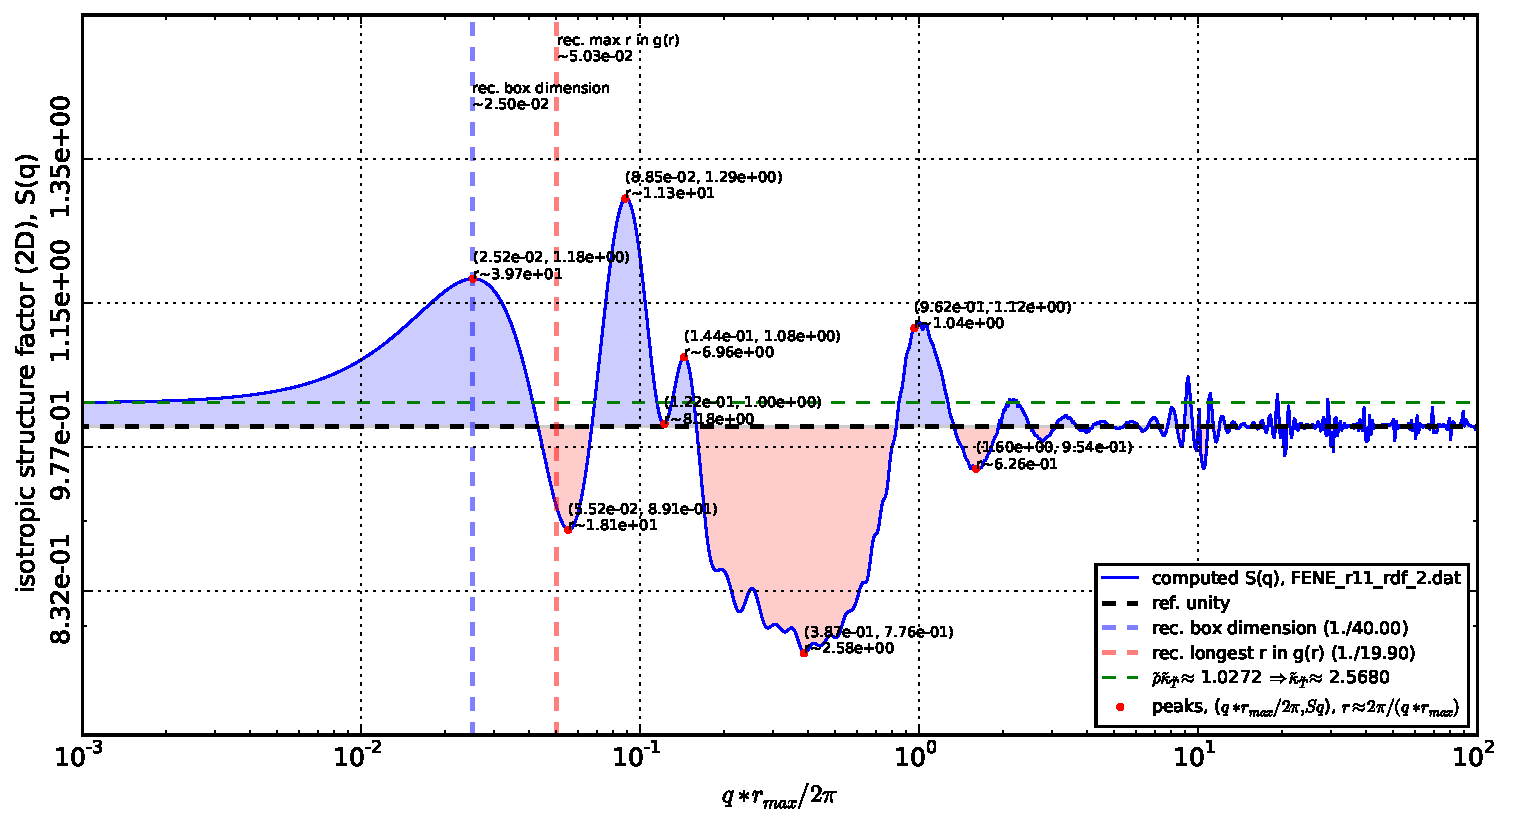
\includegraphics[height=0.3\textheight]{figures/Sq_FENE_r11_2.pdf}\\
      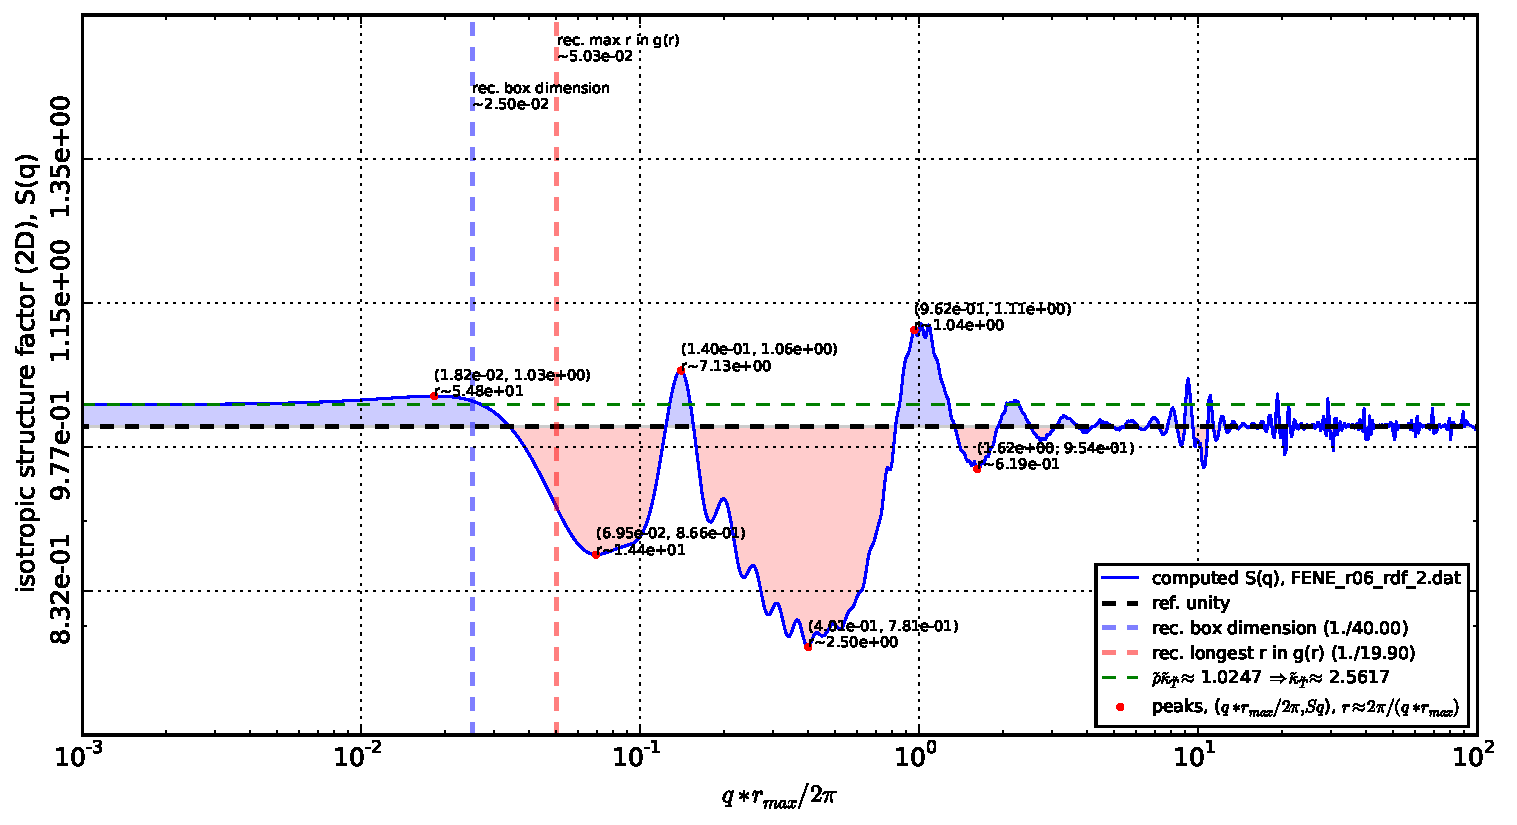
\includegraphics[height=0.3\textheight]{figures/Sq_FENE_r06_2.pdf}\\
      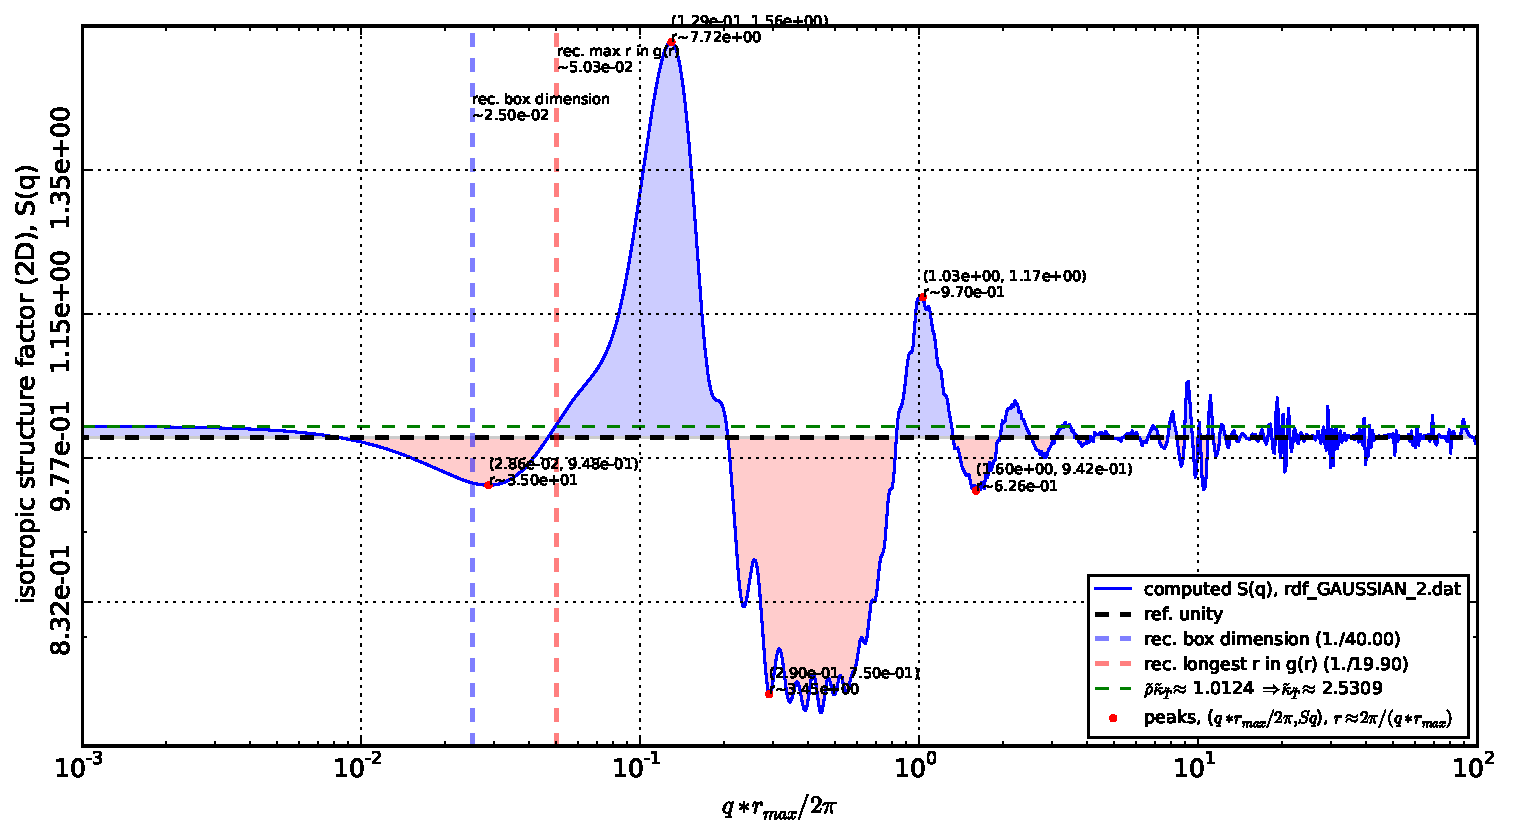
\includegraphics[height=0.3\textheight]{figures/Sq_GAUSSIAN_2.pdf}
      \caption{Computed structure factor for different conditions. From top to bottom, the figure represent FENE with r11, r06, and Gaussian, respectively.}
      \label{fig:2d_Sq_compare_all}
    \end{figure}


    \begin{figure}
      \centering
      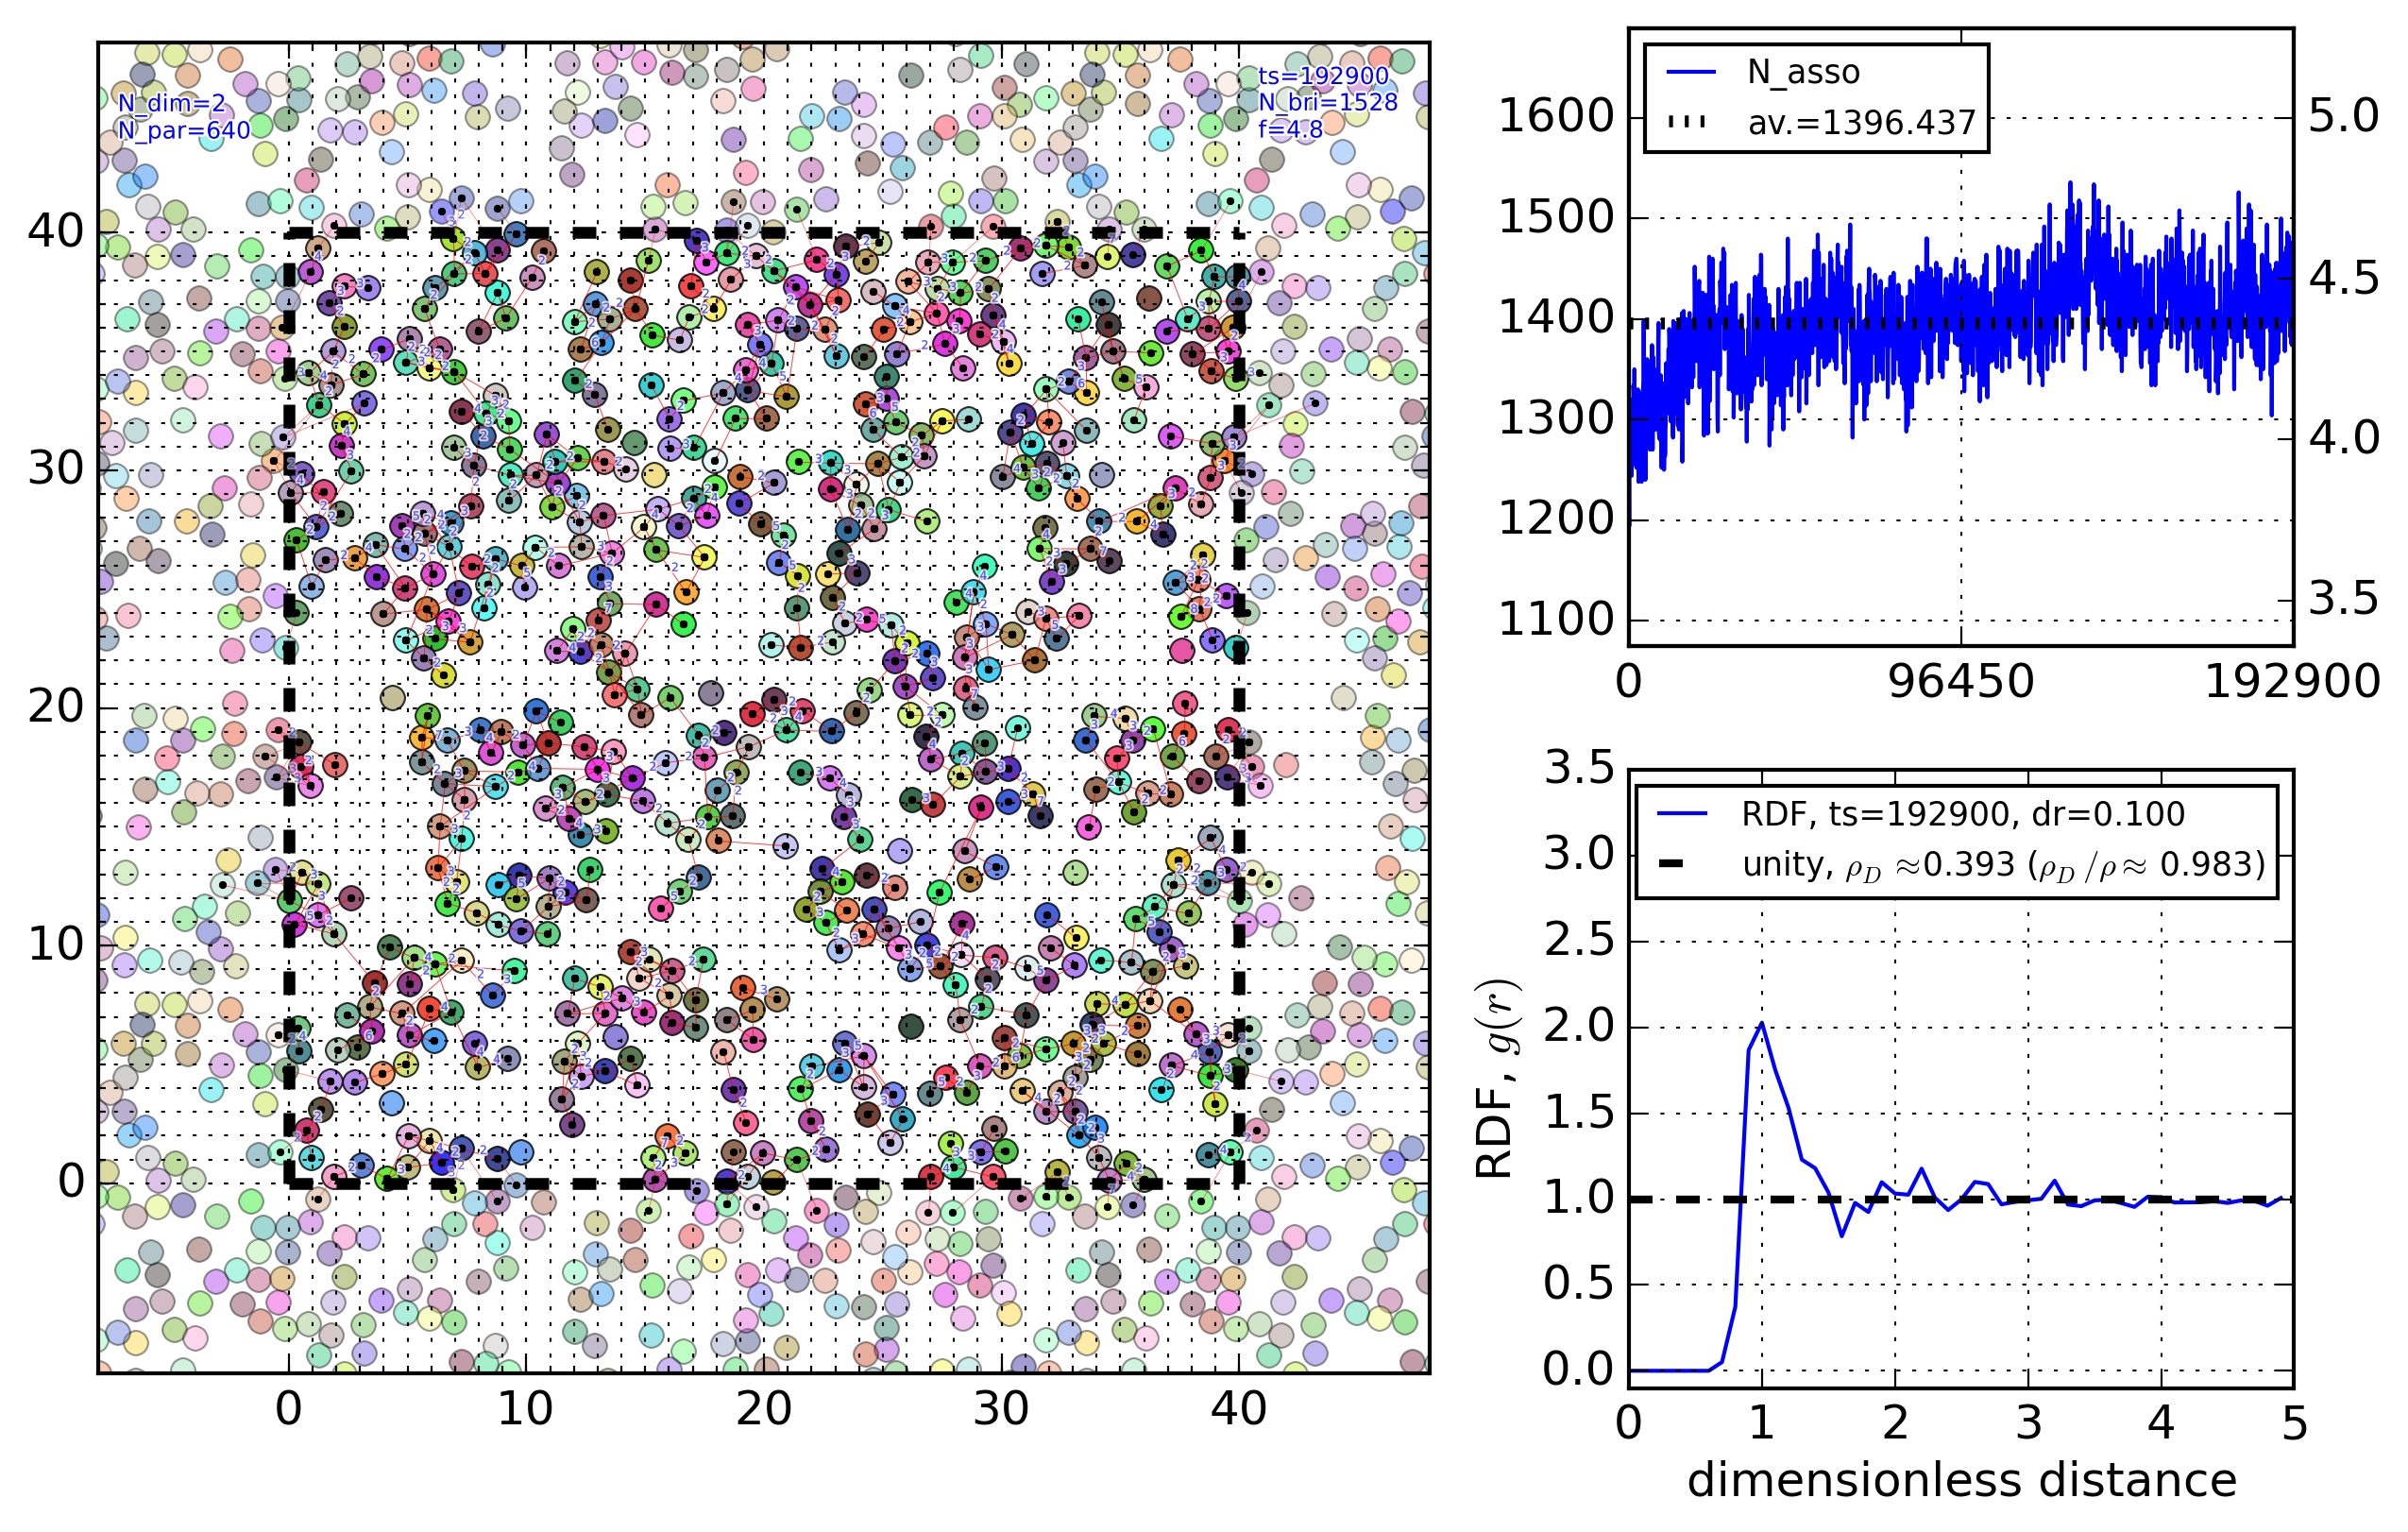
\includegraphics[height=0.3\textheight]{figures/traj_r11.png}\\
      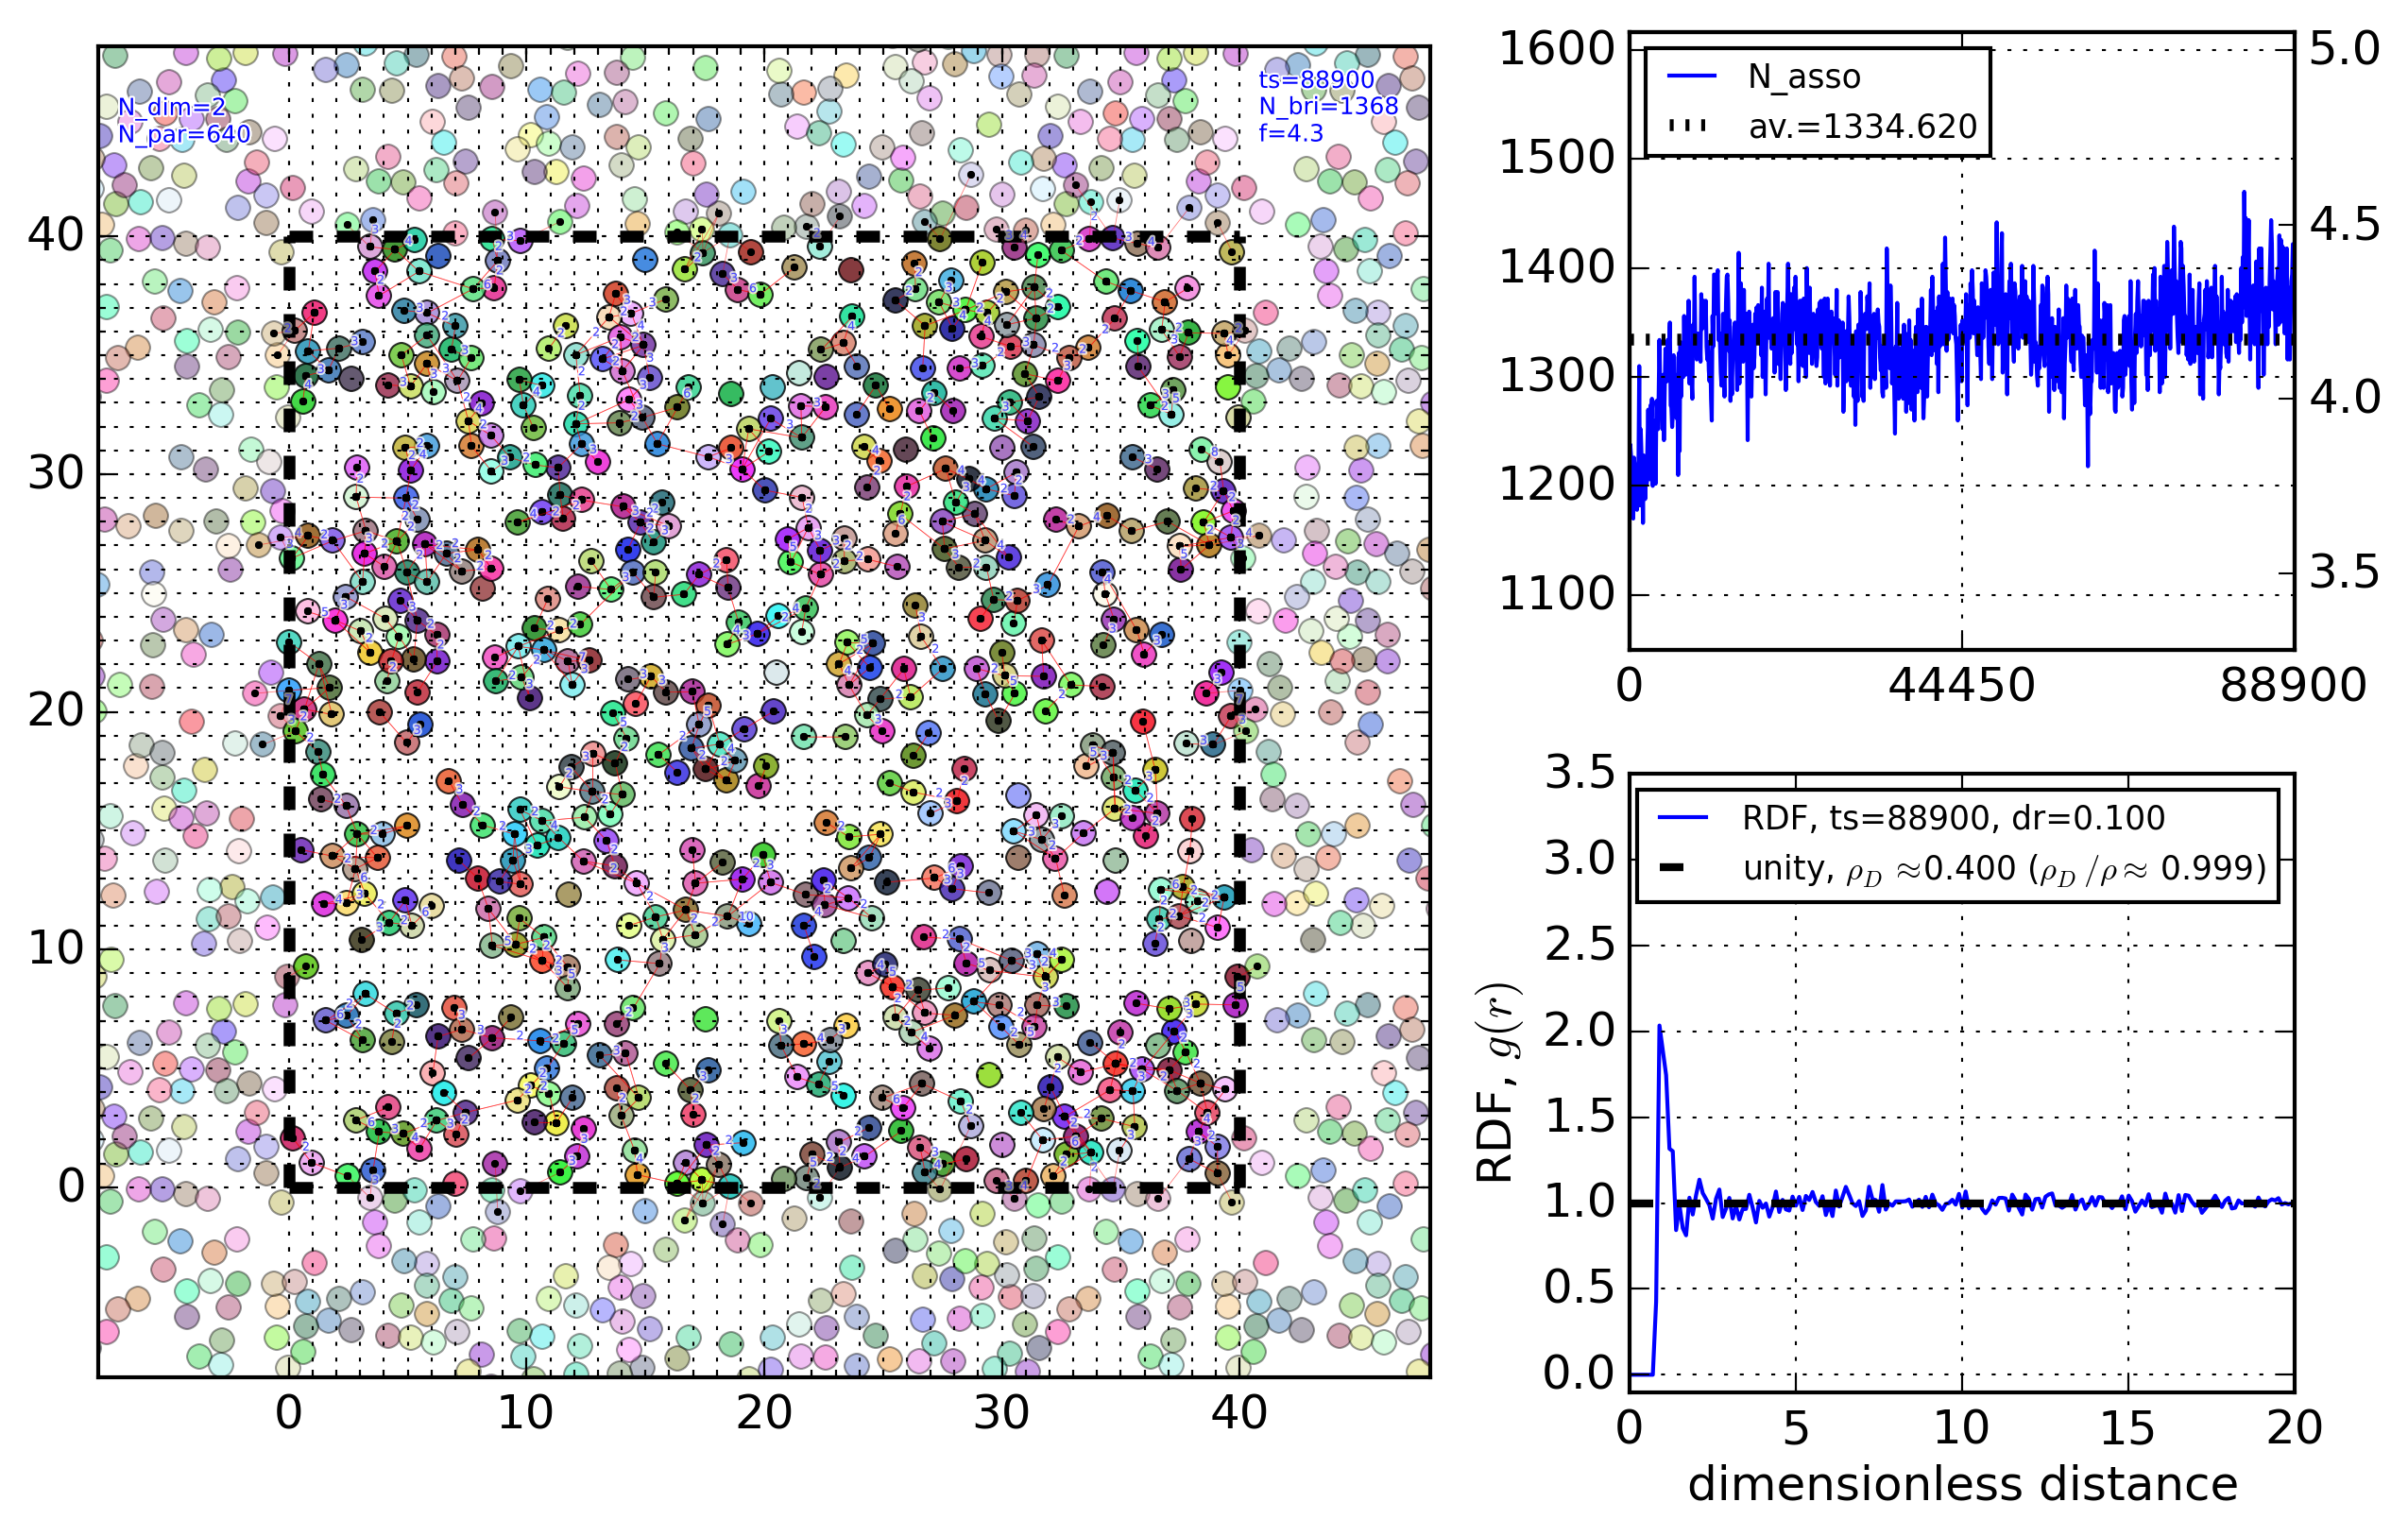
\includegraphics[height=0.3\textheight]{figures/traj_r06.png}\\
      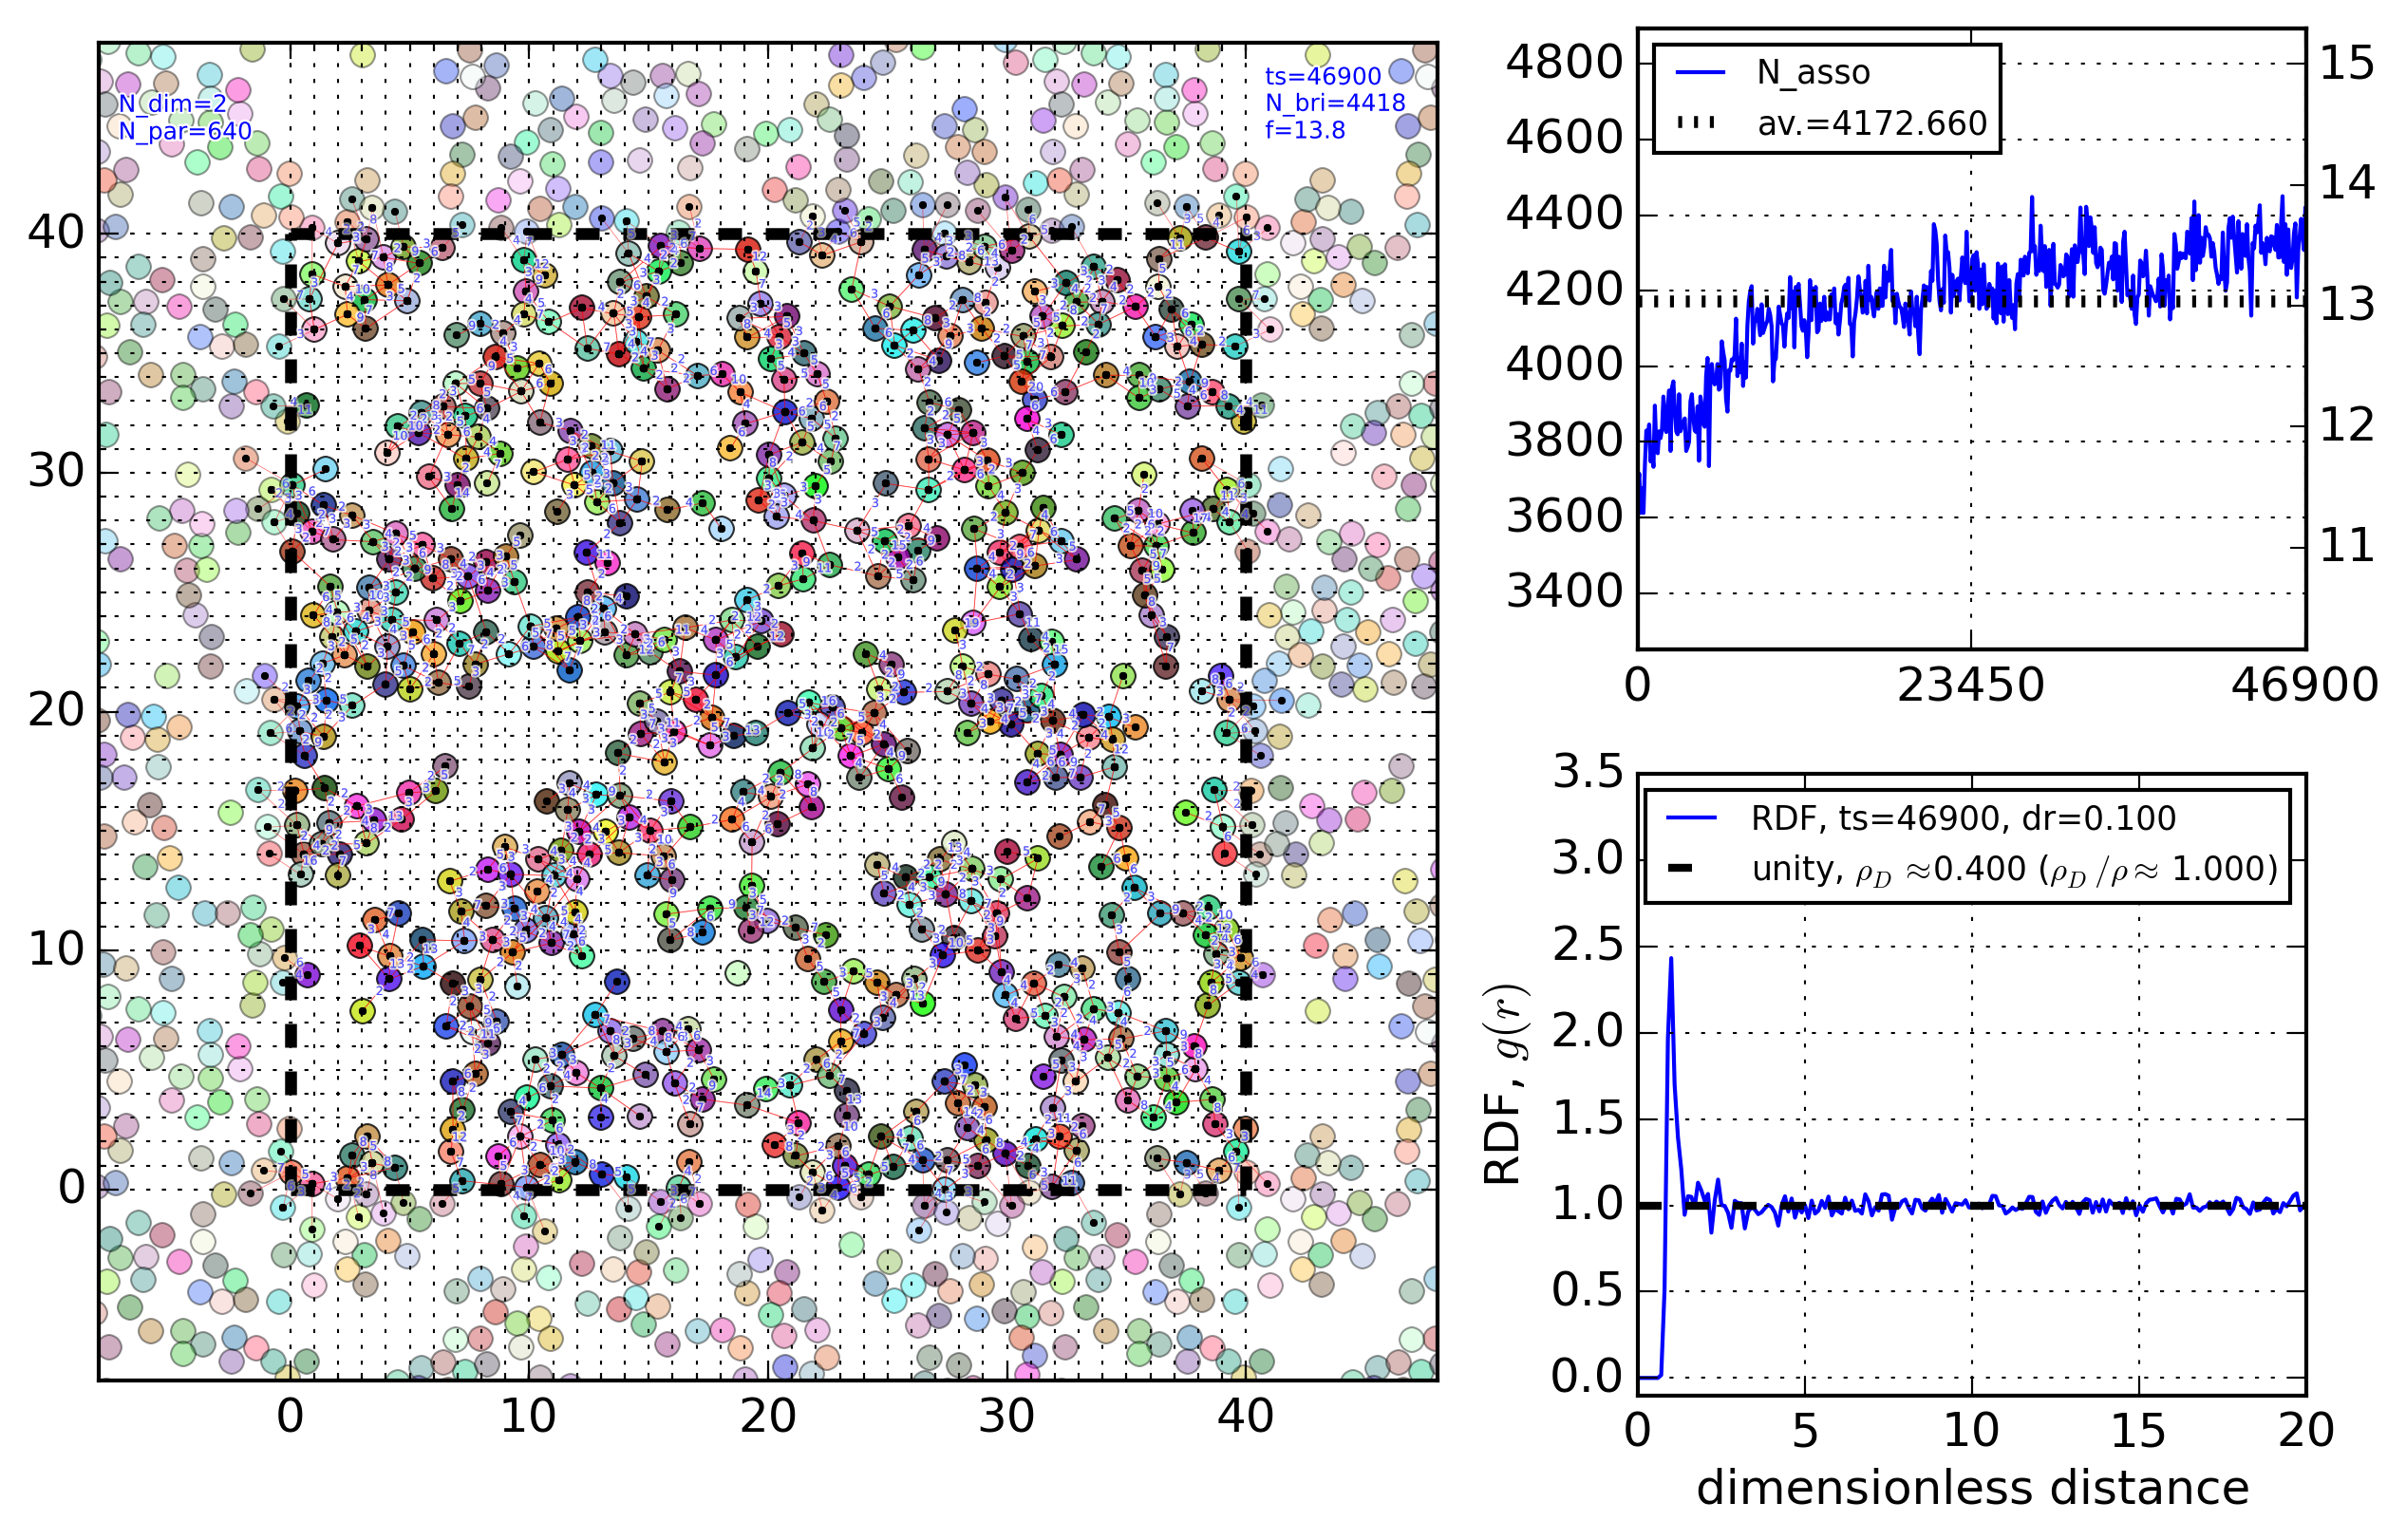
\includegraphics[height=0.3\textheight]{figures/traj_GAUSSIAN.png}
      \caption{The examples of trajectory with different conditions. From top to bottom, the figures represent FENE with ratio 11, FENE with ratio 6, and GAUSSIAN connectors, respectively. }
      \label{fig:traj_compare}
    \end{figure}
  

\end{appendices}
\newpage
\printbibliography
\end{document}
